% Options for packages loaded elsewhere
% Options for packages loaded elsewhere
\PassOptionsToPackage{unicode}{hyperref}
\PassOptionsToPackage{hyphens}{url}
\PassOptionsToPackage{dvipsnames,svgnames,x11names}{xcolor}
%
\documentclass[
  13pt,
  a4paper,
]{report}
\usepackage{xcolor}
\usepackage[top=20mm,bottom=20mm,left=30mm,right=20mm]{geometry}
\usepackage{amsmath,amssymb}
\setcounter{secnumdepth}{-\maxdimen} % remove section numbering
\usepackage{iftex}
\ifPDFTeX
  \usepackage[T1]{fontenc}
  \usepackage[utf8]{inputenc}
  \usepackage{textcomp} % provide euro and other symbols
\else % if luatex or xetex
  \usepackage{unicode-math} % this also loads fontspec
  \defaultfontfeatures{Scale=MatchLowercase}
  \defaultfontfeatures[\rmfamily]{Ligatures=TeX,Scale=1}
\fi
\usepackage{lmodern}
\ifPDFTeX\else
  % xetex/luatex font selection
\fi
% Use upquote if available, for straight quotes in verbatim environments
\IfFileExists{upquote.sty}{\usepackage{upquote}}{}
\IfFileExists{microtype.sty}{% use microtype if available
  \usepackage[]{microtype}
  \UseMicrotypeSet[protrusion]{basicmath} % disable protrusion for tt fonts
}{}
\usepackage{setspace}
\makeatletter
\@ifundefined{KOMAClassName}{% if non-KOMA class
  \IfFileExists{parskip.sty}{%
    \usepackage{parskip}
  }{% else
    \setlength{\parindent}{0pt}
    \setlength{\parskip}{6pt plus 2pt minus 1pt}}
}{% if KOMA class
  \KOMAoptions{parskip=half}}
\makeatother
% Make \paragraph and \subparagraph free-standing
\makeatletter
\ifx\paragraph\undefined\else
  \let\oldparagraph\paragraph
  \renewcommand{\paragraph}{
    \@ifstar
      \xxxParagraphStar
      \xxxParagraphNoStar
  }
  \newcommand{\xxxParagraphStar}[1]{\oldparagraph*{#1}\mbox{}}
  \newcommand{\xxxParagraphNoStar}[1]{\oldparagraph{#1}\mbox{}}
\fi
\ifx\subparagraph\undefined\else
  \let\oldsubparagraph\subparagraph
  \renewcommand{\subparagraph}{
    \@ifstar
      \xxxSubParagraphStar
      \xxxSubParagraphNoStar
  }
  \newcommand{\xxxSubParagraphStar}[1]{\oldsubparagraph*{#1}\mbox{}}
  \newcommand{\xxxSubParagraphNoStar}[1]{\oldsubparagraph{#1}\mbox{}}
\fi
\makeatother

\usepackage{color}
\usepackage{fancyvrb}
\newcommand{\VerbBar}{|}
\newcommand{\VERB}{\Verb[commandchars=\\\{\}]}
\DefineVerbatimEnvironment{Highlighting}{Verbatim}{commandchars=\\\{\}}
% Add ',fontsize=\small' for more characters per line
\usepackage{framed}
\definecolor{shadecolor}{RGB}{241,243,245}
\newenvironment{Shaded}{\begin{snugshade}}{\end{snugshade}}
\newcommand{\AlertTok}[1]{\textcolor[rgb]{0.68,0.00,0.00}{#1}}
\newcommand{\AnnotationTok}[1]{\textcolor[rgb]{0.37,0.37,0.37}{#1}}
\newcommand{\AttributeTok}[1]{\textcolor[rgb]{0.40,0.45,0.13}{#1}}
\newcommand{\BaseNTok}[1]{\textcolor[rgb]{0.68,0.00,0.00}{#1}}
\newcommand{\BuiltInTok}[1]{\textcolor[rgb]{0.00,0.23,0.31}{#1}}
\newcommand{\CharTok}[1]{\textcolor[rgb]{0.13,0.47,0.30}{#1}}
\newcommand{\CommentTok}[1]{\textcolor[rgb]{0.37,0.37,0.37}{#1}}
\newcommand{\CommentVarTok}[1]{\textcolor[rgb]{0.37,0.37,0.37}{\textit{#1}}}
\newcommand{\ConstantTok}[1]{\textcolor[rgb]{0.56,0.35,0.01}{#1}}
\newcommand{\ControlFlowTok}[1]{\textcolor[rgb]{0.00,0.23,0.31}{\textbf{#1}}}
\newcommand{\DataTypeTok}[1]{\textcolor[rgb]{0.68,0.00,0.00}{#1}}
\newcommand{\DecValTok}[1]{\textcolor[rgb]{0.68,0.00,0.00}{#1}}
\newcommand{\DocumentationTok}[1]{\textcolor[rgb]{0.37,0.37,0.37}{\textit{#1}}}
\newcommand{\ErrorTok}[1]{\textcolor[rgb]{0.68,0.00,0.00}{#1}}
\newcommand{\ExtensionTok}[1]{\textcolor[rgb]{0.00,0.23,0.31}{#1}}
\newcommand{\FloatTok}[1]{\textcolor[rgb]{0.68,0.00,0.00}{#1}}
\newcommand{\FunctionTok}[1]{\textcolor[rgb]{0.28,0.35,0.67}{#1}}
\newcommand{\ImportTok}[1]{\textcolor[rgb]{0.00,0.46,0.62}{#1}}
\newcommand{\InformationTok}[1]{\textcolor[rgb]{0.37,0.37,0.37}{#1}}
\newcommand{\KeywordTok}[1]{\textcolor[rgb]{0.00,0.23,0.31}{\textbf{#1}}}
\newcommand{\NormalTok}[1]{\textcolor[rgb]{0.00,0.23,0.31}{#1}}
\newcommand{\OperatorTok}[1]{\textcolor[rgb]{0.37,0.37,0.37}{#1}}
\newcommand{\OtherTok}[1]{\textcolor[rgb]{0.00,0.23,0.31}{#1}}
\newcommand{\PreprocessorTok}[1]{\textcolor[rgb]{0.68,0.00,0.00}{#1}}
\newcommand{\RegionMarkerTok}[1]{\textcolor[rgb]{0.00,0.23,0.31}{#1}}
\newcommand{\SpecialCharTok}[1]{\textcolor[rgb]{0.37,0.37,0.37}{#1}}
\newcommand{\SpecialStringTok}[1]{\textcolor[rgb]{0.13,0.47,0.30}{#1}}
\newcommand{\StringTok}[1]{\textcolor[rgb]{0.13,0.47,0.30}{#1}}
\newcommand{\VariableTok}[1]{\textcolor[rgb]{0.07,0.07,0.07}{#1}}
\newcommand{\VerbatimStringTok}[1]{\textcolor[rgb]{0.13,0.47,0.30}{#1}}
\newcommand{\WarningTok}[1]{\textcolor[rgb]{0.37,0.37,0.37}{\textit{#1}}}

\usepackage{longtable,booktabs,array}
\newcounter{none} % for unnumbered tables
\usepackage{calc} % for calculating minipage widths
% Correct order of tables after \paragraph or \subparagraph
\usepackage{etoolbox}
\makeatletter
\patchcmd\longtable{\par}{\if@noskipsec\mbox{}\fi\par}{}{}
\makeatother
% Allow footnotes in longtable head/foot
\IfFileExists{footnotehyper.sty}{\usepackage{footnotehyper}}{\usepackage{footnote}}
\makesavenoteenv{longtable}
\usepackage{graphicx}
\makeatletter
\newsavebox\pandoc@box
\newcommand*\pandocbounded[1]{% scales image to fit in text height/width
  \sbox\pandoc@box{#1}%
  \Gscale@div\@tempa{\textheight}{\dimexpr\ht\pandoc@box+\dp\pandoc@box\relax}%
  \Gscale@div\@tempb{\linewidth}{\wd\pandoc@box}%
  \ifdim\@tempb\p@<\@tempa\p@\let\@tempa\@tempb\fi% select the smaller of both
  \ifdim\@tempa\p@<\p@\scalebox{\@tempa}{\usebox\pandoc@box}%
  \else\usebox{\pandoc@box}%
  \fi%
}
% Set default figure placement to htbp
\def\fps@figure{htbp}
\makeatother





\setlength{\emergencystretch}{3em} % prevent overfull lines

\providecommand{\tightlist}{%
  \setlength{\itemsep}{0pt}\setlength{\parskip}{0pt}}



 


\makeatletter
\@ifpackageloaded{bookmark}{}{\usepackage{bookmark}}
\makeatother
\makeatletter
\@ifpackageloaded{caption}{}{\usepackage{caption}}
\AtBeginDocument{%
\ifdefined\contentsname
  \renewcommand*\contentsname{Table of contents}
\else
  \newcommand\contentsname{Table of contents}
\fi
\ifdefined\listfigurename
  \renewcommand*\listfigurename{List of Figures}
\else
  \newcommand\listfigurename{List of Figures}
\fi
\ifdefined\listtablename
  \renewcommand*\listtablename{List of Tables}
\else
  \newcommand\listtablename{List of Tables}
\fi
\ifdefined\figurename
  \renewcommand*\figurename{Figure}
\else
  \newcommand\figurename{Figure}
\fi
\ifdefined\tablename
  \renewcommand*\tablename{Table}
\else
  \newcommand\tablename{Table}
\fi
}
\@ifpackageloaded{float}{}{\usepackage{float}}
\floatstyle{ruled}
\@ifundefined{c@chapter}{\newfloat{codelisting}{h}{lop}}{\newfloat{codelisting}{h}{lop}[chapter]}
\floatname{codelisting}{Listing}
\newcommand*\listoflistings{\listof{codelisting}{List of Listings}}
\makeatother
\makeatletter
\makeatother
\makeatletter
\@ifpackageloaded{caption}{}{\usepackage{caption}}
\@ifpackageloaded{subcaption}{}{\usepackage{subcaption}}
\makeatother
\usepackage{bookmark}
\IfFileExists{xurl.sty}{\usepackage{xurl}}{} % add URL line breaks if available
\urlstyle{same}
\hypersetup{
  pdftitle={Đề Tài 7: Mô Hình Chấm Điểm Tín Dụng \& Thẩm Định Rủi Ro Vỡ Nợ},
  pdfauthor={Lê Thành Hiệu},
  colorlinks=true,
  linkcolor={blue},
  filecolor={Maroon},
  citecolor={Blue},
  urlcolor={Blue},
  pdfcreator={LaTeX via pandoc}}


\title{Đề Tài 7: Mô Hình Chấm Điểm Tín Dụng \& Thẩm Định Rủi Ro Vỡ Nợ}
\usepackage{etoolbox}
\makeatletter
\providecommand{\subtitle}[1]{% add subtitle to \maketitle
  \apptocmd{\@title}{\par {\large #1 \par}}{}{}
}
\makeatother
\subtitle{Báo Cáo Tiểu Luận Môn Học Dữ Liệu Lớn \& Trí Tuệ Nhân Tạo
Trong Kinh Doanh}
\author{Lê Thành Hiệu}
\date{2026-01-01}
\begin{document}
\maketitle

\renewcommand*\contentsname{Table of contents}
{
\setcounter{tocdepth}{2}
\tableofcontents
}

\setstretch{1.5}
\bookmarksetup{startatroot}

\chapter{Báo Cáo Tiểu Luận Kết Thúc Học
Phần}\label{buxe1o-cuxe1o-tiux1ec3u-luux1eadn-kux1ebft-thuxfac-hux1ecdc-phux1ea7n}

Mô Hình Chấm Điểm Tín Dụng \& Thẩm Định Rủi Ro Vỡ Nợ

\hfill\break

\bookmarksetup{startatroot}

\chapter{BÁO CÁO TIỂU LUẬN KẾT THÚC HỌC
PHẦN}\label{buxe1o-cuxe1o-tiux1ec3u-luux1eadn-kux1ebft-thuxfac-hux1ecdc-phux1ea7n-1}

\textbf{BỘ GIÁO DỤC VÀ ĐÀO TẠO}\\
\textbf{TRƯỜNG ĐẠI HỌC KINH TẾ - ĐẠI HỌC QUỐC GIA}\\
\textbf{KHOA HỆ THỐNG THÔNG TIN KINH TẾ \& PHÂN TÍCH DỮ LIỆU}

\begin{center}\rule{0.5\linewidth}{0.5pt}\end{center}

\subsection{\texorpdfstring{\textbf{BÁO CÁO TIỂU LUẬN MÔN
HỌC}}{BÁO CÁO TIỂU LUẬN MÔN HỌC}}\label{buxe1o-cuxe1o-tiux1ec3u-luux1eadn-muxf4n-hux1ecdc}

\section{\texorpdfstring{\textbf{DỮ LIỆU LỚN VÀ TRÍ TUỆ NHÂN TẠO TRONG
KINH
DOANH}}{DỮ LIỆU LỚN VÀ TRÍ TUỆ NHÂN TẠO TRONG KINH DOANH}}\label{dux1eef-liux1ec7u-lux1edbn-vuxe0-truxed-tuux1ec7-nhuxe2n-tux1ea1o-trong-kinh-doanh}

\subsection{\texorpdfstring{\emph{(BIG DATA ANALYTICS \& ARTIFICIAL
INTELLIGENCE IN
BUSINESS)}}{(BIG DATA ANALYTICS \& ARTIFICIAL INTELLIGENCE IN BUSINESS)}}\label{big-data-analytics-artificial-intelligence-in-business}

\begin{center}\rule{0.5\linewidth}{0.5pt}\end{center}

\subsection{\texorpdfstring{\textbf{ĐỀ TÀI NGHIÊN
CỨU:}}{ĐỀ TÀI NGHIÊN CỨU:}}\label{ux111ux1ec1-tuxe0i-nghiuxean-cux1ee9u}

\bookmarksetup{startatroot}

\chapter{\texorpdfstring{\textbf{MÔ HÌNH CHẤM ĐIỂM TÍN DỤNG VÀ THẨM ĐỊNH
RỦI RO VỠ NỢ TRONG LĨNH VỰC NGÂN HÀNG VÀ
FINTECH}}{MÔ HÌNH CHẤM ĐIỂM TÍN DỤNG VÀ THẨM ĐỊNH RỦI RO VỠ NỢ TRONG LĨNH VỰC NGÂN HÀNG VÀ FINTECH}}\label{muxf4-huxecnh-chux1ea5m-ux111iux1ec3m-tuxedn-dux1ee5ng-vuxe0-thux1ea9m-ux111ux1ecbnh-rux1ee7i-ro-vux1ee1-nux1ee3-trong-lux129nh-vux1ef1c-nguxe2n-huxe0ng-vuxe0-fintech}

\subsection{\texorpdfstring{\emph{(LOAN DEFAULT PREDICTION \& CREDIT
SCORING IN BANKING AND
FINTECH)}}{(LOAN DEFAULT PREDICTION \& CREDIT SCORING IN BANKING AND FINTECH)}}\label{loan-default-prediction-credit-scoring-in-banking-and-fintech}

\begin{center}\rule{0.5\linewidth}{0.5pt}\end{center}

\textbf{Giảng viên hướng dẫn:} TS. Trần Mạnh Tường\\
\textbf{Sinh viên thực hiện:} Lê Thành Hiệu\\
\textbf{Mã số sinh viên:} {[}Điền MSSV tại đây{]}\\
\textbf{Lớp / Khóa học:} Big Data Analytics \& AI - Khóa 2026\\
\textbf{Chuyên ngành:} Hệ thống Thông tin Quản lý / Phân tích Kinh doanh

\begin{center}\rule{0.5\linewidth}{0.5pt}\end{center}

\textbf{TP. Hồ Chí Minh, năm 2026}

\newpage

\begin{center}\rule{0.5\linewidth}{0.5pt}\end{center}

\section{LỜI CAM ĐOAN}\label{lux1eddi-cam-ux111oan}

Tôi xin cam đoan rằng bài tiểu luận kết thúc học phần với đề tài
\textbf{``Mô hình chấm điểm tín dụng và thẩm định rủi ro vỡ nợ trong
lĩnh vực Ngân hàng và FinTech''} là công trình nghiên cứu độc lập của cá
nhân tôi dưới sự hướng dẫn khoa học của \textbf{TS. Trần Mạnh Tường}.

Toàn bộ số liệu phân tích, kết quả mô phỏng thực nghiệm và các luận điểm
trình bày trong báo cáo hoàn toàn trung thực, khách quan và được thu
thập, xử lý từ dữ liệu thực tế 2,260,701 khoản vay của nền tảng
LendingClub. Các tài liệu tham khảo, các lý thuyết tài chính - ngân hàng
và nghiên cứu khoa học của các tác giả khác đều được trích dẫn nguồn gốc
đầy đủ theo đúng quy chuẩn học thuật hiện hành.

\emph{TP. Hồ Chí Minh, năm 2026}\\
\textbf{Sinh viên thực hiện}\\
\emph{(Ký và ghi rõ họ tên)}

\textbf{Lê Thành Hiệu}

\newpage

\begin{center}\rule{0.5\linewidth}{0.5pt}\end{center}

\section{LỜI CẢM ƠN}\label{lux1eddi-cux1ea3m-ux1a1n}

Để hoàn thành bài tiểu luận nghiên cứu này, trước hết em xin bày tỏ lòng
biết ơn sâu sắc và chân thành nhất đến \textbf{TS. Trần Mạnh Tường},
giảng viên phụ trách học phần \emph{Dữ liệu lớn và Trí tuệ nhân tạo
trong Kinh doanh}. Thầy đã tận tình truyền đạt những kiến thức chuyên
môn sâu rộng về kiến trúc dữ liệu phân tán, khoa học dữ liệu hiện đại và
các phương pháp ứng dụng trí tuệ nhân tạo vào thực tiễn kinh tế - tài
chính. Những lời chỉ dẫn, định hướng khoa học và phản biện quý báu của
Thầy trong suốt quá trình học tập là tiền đề quan trọng giúp em hoàn
thiện đồ án này một cách chỉn chu và đúng đắn.

Em cũng xin gửi lời cảm ơn chân thành đến Ban Giám hiệu nhà trường, các
Quý Thầy Cô trong Khoa Hệ thống Thông tin Kinh tế đã tạo điều kiện học
tập tốt nhất, cung cấp môi trường nghiên cứu và cơ sở vật chất hiện đại
phục vụ cho môn học.

\emph{Kính chúc Thầy luôn dồi dào sức khỏe, hạnh phúc và gặt hái được
nhiều thành công hơn nữa trong sự nghiệp giảng dạy và nghiên cứu khoa
học cao quý!}

\newpage

\begin{center}\rule{0.5\linewidth}{0.5pt}\end{center}

\section{TÓM TẮT ĐỀ TÀI
(ABSTRACT)}\label{tuxf3m-tux1eaft-ux111ux1ec1-tuxe0i-abstract}

\subsection{Tóm tắt tiếng
Việt}\label{tuxf3m-tux1eaft-tiux1ebfng-viux1ec7t}

Trong bối cảnh bùng nổ của dịch vụ tài chính số (FinTech) và ngân hàng
bán lẻ, rủi ro vỡ nợ (Loan Default Risk) luôn là mối đe dọa trực tiếp
đối với tính an toàn vốn và khả năng sinh lời của các tổ chức tín dụng.
Phương pháp chấm điểm tín dụng truyền thống bộc lộ nhiều hạn chế về tốc
độ xử lý, chi phí nhân sự và độ chính xác khi đối mặt với quy mô hồ sơ
vay trực tuyến ngày càng lớn. Đề tài nghiên cứu này tập trung xây dựng
một giải pháp toàn diện ứng dụng công nghệ \textbf{Dữ liệu lớn (Big
Data)} trên nền tảng \textbf{Databricks Lakehouse} kết hợp thuật toán
học máy phân tán \textbf{Random Forest Classifier (Spark MLlib)} nhằm tự
động hóa quy trình thẩm định tín dụng và ra quyết định cấp vốn.

Dữ liệu thực nghiệm quy mô lớn bao gồm 2,260,701 khoản vay (hơn 2.26
triệu bản ghi, 1.6 GB) từ nền tảng tín dụng LendingClub (giai đoạn 2007
- 2018Q4), được xử lý phân tán xuyên suốt qua kiến trúc Medallion 3 tầng
(Bronze \(\rightarrow\) Silver \(\rightarrow\) Gold), áp dụng các kỹ
thuật làm sạch dữ liệu, xử lý ngoại lai, kỹ nghệ đặc trưng tài chính
(DTI, CBI) và phân tích bằng Spark SQL. Mô hình học máy phân tán được
tinh chỉnh qua cơ chế kiểm định chéo (3-Fold Cross-Validation), đạt chỉ
số phân loại vượt trội với \textbf{ROC-AUC = 0.8745}, độ nhạy phát hiện
nợ xấu (Recall) đạt 84.04\% và độ chính xác (Precision) đạt 66.20\%. Từ
kết quả xác suất vỡ nợ, đề tài xây dựng động cơ ra quyết định chuẩn hóa
theo điểm tín dụng FICO Score (\(300 - 850\)), thiết lập ma trận phân
tầng 4 nhóm rủi ro dựa trên chỉ số Youden's J Statistic và chuẩn mực
Basel II, đồng thời đề xuất mô hình định giá lãi suất theo rủi ro
(Risk-Based Pricing Model) với các mức lãi suất 8.5\%, 11.5\%, 14.5\%.
Hệ thống cho phép tự động hóa phê duyệt trên 75\% hồ sơ vay trong thời
gian dưới 3 phút, giúp giảm tỷ lệ nợ xấu tổng thể xuống dưới 4.2\% và
tiết kiệm hàng tỷ đồng chi phí trích lập dự phòng tổn thất tín dụng.

\subsection{Abstract in English}\label{abstract-in-english}

In the era of digital banking and FinTech expansion, loan default risk
poses a critical threat to capital adequacy and profitability of credit
institutions. Traditional credit underwriting methods exhibit
significant drawbacks regarding turnaround time, operational costs, and
subjective biases when processing surging volumes of online loan
applications. This research develops an end-to-end Big Data solution
utilizing the \textbf{Databricks Lakehouse Platform} combined with
distributed machine learning via \textbf{Random Forest Classifier (Spark
MLlib)} to automate credit scoring and loan origination decision-making.

A large-scale empirical dataset of 2,260,701 loan records (2.26 million
records, 1.6 GB) from the LendingClub platform (2007 - 2018Q4) was
processed in a distributed manner across the 3-tier Medallion
Architecture (Bronze \(\rightarrow\) Silver \(\rightarrow\) Gold),
incorporating data cleaning, outlier treatment, financial feature
engineering (DTI, CBI), and distributed analytics via Spark SQL. The
machine learning pipeline was hyperparameter-tuned using 3-Fold
Cross-Validation, achieving superior predictive power with
\textbf{ROC-AUC = 0.8745}, a default recall of 84.04\%, and overall
accuracy of 87.16\%. Based on predicted default probabilities, the
system implements a decision engine that converts probabilities into
standardized FICO Scores (\(300 - 850\)), establishes a 4-tier risk
segmentation matrix underpinned by Youden's J Statistic and Basel II
standards, and formulates a Risk-Based Pricing Model with suggested
interest rates of 8.5\%, 11.5\%, and 14.5\% per annum. The proposed
architecture enables straight-through processing (STP) for over 75\% of
loan applications in under 3 minutes, effectively reducing portfolio
Non-Performing Loans (NPL) below 4.2\% and mitigating credit loss
provisioning expenses.

\newpage

\begin{center}\rule{0.5\linewidth}{0.5pt}\end{center}

\section{MỤC LỤC BÁO CÁO (TABLE OF
CONTENTS)}\label{mux1ee5c-lux1ee5c-buxe1o-cuxe1o-table-of-contents}

\begin{itemize}
\tightlist
\item
  \textbf{TRANG BÌA \& THÔNG TIN DỰ ÁN}
\item
  \textbf{LỜI CAM ĐOAN}
\item
  \textbf{LỜI CẢM ƠN}
\item
  \textbf{TÓM TẮT ĐỀ TÀI (ABSTRACT)}
\item
  \textbf{DANH MỤC CÁC CHỮ VIẾT TẮT}
\item
  \textbf{DANH MỤC BẢNG BIỂU}
\item
  \textbf{DANH MỤC HÌNH VẼ \& BIỂU ĐỒ}
\item
  \textbf{CHƯƠNG 1: TỔNG QUAN VỀ BÀI TOÁN \& ĐẶT VẤN ĐỀ}

  \begin{itemize}
  \tightlist
  \item
    1.1. Bối cảnh ngành Tài chính - Ngân hàng và FinTech trong kỷ nguyên
    số
  \item
    1.2. Hạn chế của phương pháp thẩm định tín dụng truyền thống
  \item
    1.3. Tính cấp thiết của đề tài và Mục tiêu nghiên cứu
  \item
    1.4. Phân tích đặc tính Dữ liệu lớn (Big Data) theo mô hình 5Vs
  \item
    1.5. Giới thiệu Bộ dữ liệu nghiên cứu và Phạm vi đề tài
  \item
    1.6. Kết cấu tổng quan của bài tiểu luận
  \end{itemize}
\item
  \textbf{CHƯƠNG 2: KIẾN TRÚC LUỒNG DỮ LIỆU LAKEHOUSE (MEDALLION
  ARCHITECTURE)}

  \begin{itemize}
  \tightlist
  \item
    2.1. Cơ sở lý luận về Kiến trúc Dữ liệu lớn: Từ Data Warehouse, Data
    Lake đến Lakehouse
  \item
    2.2. Nền tảng Apache Spark và Định dạng lưu trữ phân tán Delta Lake
  \item
    2.3. Thiết kế Kiến trúc Huy chương Medallion 3 tầng (Bronze - Silver
    - Gold)
  \item
    2.4. Sơ đồ luồng dữ liệu phân tán toàn diện (Data Pipeline Workflow)
  \item
    2.5. Quản trị dữ liệu (Data Governance) và Tuân thủ an toàn vốn theo
    chuẩn Basel II/III
  \end{itemize}
\item
  \textbf{CHƯƠNG 3: XỬ LÝ \& PHÂN TÍCH DỮ LIỆU LỚN VỚI PYSPARK VÀ SPARK
  SQL}

  \begin{itemize}
  \tightlist
  \item
    3.1. Quy trình Thu thập và Nạp dữ liệu thô (Bronze Layer Ingestion)
  \item
    3.2. Phương pháp Tiền xử lý và Nâng cao chất lượng Dữ liệu phân tán
    (Silver Layer)
  \item
    3.3. Kỹ nghệ đặc trưng tài chính (Financial Feature Engineering)
  \item
    3.4. Phân tích Khám phá Dữ liệu lớn (Exploratory Data Analysis -
    EDA) bằng Spark SQL
  \item
    3.5. Ứng dụng Window Functions trong phân tích vị thế thu nhập và
    rủi ro tín dụng tương đối
  \end{itemize}
\item
  \textbf{CHƯƠNG 4: XÂY DỰNG MÔ HÌNH HỌC MÁY PHÂN TÁN VỚI SPARK MLLIB}

  \begin{itemize}
  \tightlist
  \item
    4.1. Cơ sở lý thuyết của Thuật toán Random Forest Classifier
  \item
    4.2. Thiết kế Chuỗi Pipeline Đặc trưng phân tán (Spark MLlib Feature
    Pipeline)
  \item
    4.3. Phương pháp Huấn luyện và Tinh chỉnh Siêu tham số
    (Hyperparameter Tuning)
  \item
    4.4. Đánh giá Đa chiều Hiệu năng Mô hình (ROC-AUC, Confusion Matrix,
    Precision, Recall)
  \item
    4.5. Phân tích Tầm quan trọng của Đặc trưng (Feature Importance
    Analysis)
  \end{itemize}
\item
  \textbf{CHƯƠNG 5: PHÂN TÍCH Ý NGHĨA NGHIỆP VỤ \& ĐỀ XUẤT CHIẾN LƯỢC
  QUẢN TRỊ}

  \begin{itemize}
  \tightlist
  \item
    5.1. Động cơ Ra quyết định: Quy đổi Điểm tín dụng FICO Score
  \item
    5.2. Ma trận Phân tầng Rủi ro và Cơ sở Khoa học xác lập Ngưỡng cắt
  \item
    5.3. Mô hình Định giá Lãi suất theo Rủi ro (Risk-Based Pricing
    Framework)
  \item
    5.4. Chính sách Hạn mức Linh hoạt và Cơ chế ``Cứu khoản vay''
  \item
    5.5. Đánh giá Tác động Tài chính, Hiệu quả Vận hành và Lợi ích Kinh
    tế (ROI)
  \item
    5.6. Khuyến nghị Quản trị Chiến lược cho Ban Điều hành Ngân hàng và
    FinTech
  \end{itemize}
\item
  \textbf{TÀI LIỆU THAM KHẢO}
\end{itemize}

\newpage

\begin{center}\rule{0.5\linewidth}{0.5pt}\end{center}

\section{DANH MỤC CÁC CHỮ VIẾT TẮT (GLOSSARY OF
ACRONYMS)}\label{danh-mux1ee5c-cuxe1c-chux1eef-viux1ebft-tux1eaft-glossary-of-acronyms}

{\def\LTcaptype{none} % do not increment counter
\begin{longtable}[]{@{}
  >{\raggedright\arraybackslash}p{(\linewidth - 4\tabcolsep) * \real{0.3333}}
  >{\raggedright\arraybackslash}p{(\linewidth - 4\tabcolsep) * \real{0.3333}}
  >{\raggedright\arraybackslash}p{(\linewidth - 4\tabcolsep) * \real{0.3333}}@{}}
\toprule\noalign{}
\begin{minipage}[b]{\linewidth}\raggedright
Từ Viết Tắt
\end{minipage} & \begin{minipage}[b]{\linewidth}\raggedright
Tên Tiếng Anh Đầy Đủ
\end{minipage} & \begin{minipage}[b]{\linewidth}\raggedright
Nghĩa Tiếng Việt / Giải Thích
\end{minipage} \\
\midrule\noalign{}
\endhead
\bottomrule\noalign{}
\endlastfoot
\textbf{ACID} & Atomicity, Consistency, Isolation, Durability & Bốn
thuộc tính toàn vẹn của hệ quản trị cơ sở dữ liệu \\
\textbf{AI} & Artificial Intelligence & Trí tuệ nhân tạo \\
\textbf{AUC} & Area Under the ROC Curve & Diện tích dưới đường cong
ROC \\
\textbf{BCBS} & Basel Committee on Banking Supervision & Ủy ban Basel về
Giám sát Ngân hàng \\
\textbf{CBI} & Credit Burden Index & Chỉ số gánh nặng tín dụng có trọng
số thâm niên công tác \\
\textbf{CIC} & Credit Information Center & Trung tâm Thông tin Tín dụng
Quốc gia Việt Nam \\
\textbf{COF} & Cost of Funds & Chi phí huy động vốn của ngân hàng \\
\textbf{DTI} & Debt-to-Income Ratio & Tỷ lệ tổng dư nợ trên thu nhập
hàng năm \\
\textbf{EAD} & Exposure at Default & Tổng dư nợ chịu rủi ro tại thời
điểm vỡ nợ \\
\textbf{EL} & Expected Loss & Tổn thất tín dụng kỳ vọng
(\(EL = PD \times LGD \times EAD\)) \\
\textbf{FICO} & Fair Isaac Corporation Score & Thang điểm tín nhiệm cá
nhân tiêu chuẩn (\(300 - 850\)) \\
\textbf{FN} & False Negative & Sai lầm loại 2 (Dự báo không vỡ nợ nhưng
thực tế vỡ nợ) \\
\textbf{FP} & False Positive & Sai lầm loại 1 (Dự báo vỡ nợ nhưng thực
tế trả đúng hạn) \\
\textbf{LGD} & Loss Given Default & Tỷ lệ tổn thất thực tế khi xảy ra
biến cố vỡ nợ \\
\textbf{ML} & Machine Learning & Học máy \\
\textbf{NIM} & Net Interest Margin & Biên lãi thuần của tổ chức tín
dụng \\
\textbf{NPL} & Non-Performing Loan & Tỷ lệ nợ xấu (quá hạn trên 90
ngày) \\
\textbf{OPEX} & Operating Expenses & Chi phí vận hành hoạt động \\
\textbf{PD} & Probability of Default & Xác suất vỡ nợ của khoản vay \\
\textbf{ROC} & Receiver Operating Characteristic & Đường cong đặc trưng
hoạt động phân loại \\
\textbf{STP} & Straight-Through Processing & Quy trình xử lý và phê
duyệt tự động thông suốt \\
\textbf{TN} & True Negative & Dự báo đúng khách hàng trả nợ tốt \\
\textbf{TP} & True Positive & Dự báo chính xác khách hàng vỡ nợ \\
\end{longtable}
}

\newpage

\begin{center}\rule{0.5\linewidth}{0.5pt}\end{center}

\section{DANH MỤC BẢNG BIỂU (LIST OF
TABLES)}\label{danh-mux1ee5c-bux1ea3ng-biux1ec3u-list-of-tables}

\begin{itemize}
\tightlist
\item
  \textbf{Bảng 1.1:} Phân tích đặc tính Dữ liệu lớn (Big Data) theo mô
  hình 5Vs trong Đề tài Chấm điểm Tín dụng.
\item
  \textbf{Bảng 1.2:} Mô tả chi tiết 12 thuộc tính kinh tế - tài chính
  trong Bộ dữ liệu lớn LendingClub (2,260,701 bản ghi).
\item
  \textbf{Bảng 2.1:} So sánh ưu nhược điểm giữa Data Warehouse, Data
  Lake và Databricks Lakehouse.
\item
  \textbf{Bảng 2.2:} Phân định chức năng, nguyên tắc và công nghệ giữa 3
  tầng kiến trúc Medallion (Bronze, Silver, Gold).
\item
  \textbf{Bảng 3.1:} Kế hoạch làm sạch và chuẩn hóa dữ liệu tại Tầng
  Silver.
\item
  \textbf{Bảng 3.2:} Thống kê tỷ lệ nợ xấu (NPL Rate) và quy mô tín dụng
  theo Mục đích sử dụng vốn (Loan Intent).
\item
  \textbf{Bảng 3.3:} Ma trận phân bố rủi ro theo Hạng khoản vay (Loan
  Grade) và Tình trạng sở hữu nhà ở (Home Ownership).
\item
  \textbf{Bảng 4.1:} Không gian tìm kiếm siêu tham số trong bộ tinh
  chỉnh ParamGridBuilder.
\item
  \textbf{Bảng 4.2:} Ma trận nhầm lẫn (Confusion Matrix) của mô hình
  Random Forest trên tập kiểm thử 452,140 hồ sơ.
\item
  \textbf{Bảng 4.3:} Bảng tổng hợp các chỉ số đánh giá hiệu năng phân
  loại (Accuracy, Precision, Recall, F1, ROC-AUC).
\item
  \textbf{Bảng 4.4:} Xếp hạng mức độ quan trọng của các biến đặc trưng
  (Feature Importance Ranking).
\item
  \textbf{Bảng 5.1:} Bảng quy đổi Log-Odds từ xác suất vỡ nợ (\(p\))
  sang Thang điểm tín dụng FICO Score.
\item
  \textbf{Bảng 5.2:} Ma trận Phê duyệt Tín dụng Tự động và Chính sách
  Hạn mức theo 4 Phân tầng Rủi ro.
\item
  \textbf{Bảng 5.3:} Cấu thành chi phí lãi suất theo mô hình Risk-Based
  Pricing chuẩn mực ngân hàng.
\item
  \textbf{Bảng 5.4:} Minh họa kết quả phê duyệt và giải ngân tự động
  trên 4 hồ sơ khách hàng thực tế tại Tầng Gold.
\end{itemize}

\newpage

\begin{center}\rule{0.5\linewidth}{0.5pt}\end{center}

\section{DANH MỤC HÌNH VẼ \& BIỂU ĐỒ (LIST OF
FIGURES)}\label{danh-mux1ee5c-huxecnh-vux1ebd-biux1ec3u-ux111ux1ed3-list-of-figures}

\begin{itemize}
\tightlist
\item
  \textbf{Hình 2.1:} Sơ đồ kiến trúc xử lý luồng dữ liệu Lakehouse theo
  mô hình Huy chương Medallion (Mermaid Diagram).
\item
  \textbf{Hình 3.1:} Đánh giá tỷ lệ dữ liệu khuyết thiếu Tầng Bronze
  (Missing Values Analysis).
\item
  \textbf{Hình 3.2:} Tỷ lệ nợ xấu NPL theo Mục đích vay và Tình trạng
  nhà ở Tầng Silver.
\item
  \textbf{Hình 4.1:} Đường cong ROC và so sánh hiệu năng các mô hình máy
  học (ROC-AUC = 0.8745).
\item
  \textbf{Hình 4.2:} Ma trận nhầm lẫn (Confusion Matrix) của mô hình
  trên 452,140 hồ sơ kiểm thử.
\item
  \textbf{Hình 5.1:} Cơ cấu phân tầng rủi ro tín dụng (Donut Chart) và
  Quyết định phê duyệt tự động (Bar Chart).
\end{itemize}

\bookmarksetup{startatroot}

\chapter{Chương 1: Tổng Quan Về Bài Toán \& Đặt Vấn
Đề}\label{chux1b0ux1a1ng-1-tux1ed5ng-quan-vux1ec1-buxe0i-touxe1n-ux111ux1eb7t-vux1ea5n-ux111ux1ec1}

Bối cảnh Ngân hàng số, FinTech và Mô hình 5Vs Dữ liệu lớn

\hfill\break

\bookmarksetup{startatroot}

\chapter{CHƯƠNG 1: TỔNG QUAN VỀ BÀI TOÁN \& ĐẶT VẤN
ĐỀ}\label{chux1b0ux1a1ng-1-tux1ed5ng-quan-vux1ec1-buxe0i-touxe1n-ux111ux1eb7t-vux1ea5n-ux111ux1ec1-1}

\begin{center}\rule{0.5\linewidth}{0.5pt}\end{center}

\section{1.1. Bối cảnh ngành Tài chính - Ngân hàng và FinTech trong kỷ
nguyên
số}\label{bux1ed1i-cux1ea3nh-nguxe0nh-tuxe0i-chuxednh---nguxe2n-huxe0ng-vuxe0-fintech-trong-kux1ef7-nguyuxean-sux1ed1}

Trong nền kinh tế thị trường hiện đại, hệ thống tài chính - ngân hàng
giữ vai trò huyết mạch trong việc dẫn truyền dòng vốn từ các chủ thể
tiết kiệm đến các chủ thể có nhu cầu đầu tư và tiêu dùng {[}1{]}. Phân
khúc tín dụng bán lẻ (Retail Banking) và cho vay tiêu dùng cá nhân
(Consumer Lending) đã chứng kiến tốc độ tăng trưởng bùng nổ, đặc biệt là
khi chuyển dịch từ các kênh giao dịch tại quầy sang các nền tảng số hóa
(Digital Banking, Mobile Banking và các ứng dụng FinTech) {[}2{]}. Khách
hàng ngày nay kỳ vọng những trải nghiệm vay vốn tức thì (Instant Credit
/ Buy Now Pay Later - BNPL), quy trình đăng ký 100\% trực tuyến và thời
gian phê duyệt giải ngân chỉ tính bằng phút {[}3{]}.

Tuy nhiên, song hành cùng cơ hội mở rộng biên lãi thuần (Net Interest
Margin - NIM), hoạt động cấp tín dụng luôn tiềm ẩn bản chất cố hữu là
\textbf{rủi ro tín dụng (Credit Risk)} mà đỉnh điểm là \textbf{biến cố
vỡ nợ (Loan Default)} {[}4{]}. Theo Ủy ban Basel về Giám sát Ngân hàng
(BCBS), biến cố vỡ nợ xảy ra khi người vay không thực hiện nghĩa vụ trả
nợ gốc hoặc lãi theo thỏa thuận hợp đồng sau thời hạn quy định (quá hạn
từ 90 ngày trở lên) {[}5{]}. Sự gia tăng của tỷ lệ nợ xấu
(Non-Performing Loans - NPL) không chỉ bào mòn nguồn vốn tự có của ngân
hàng thông qua chi phí trích lập dự phòng tổn thất, mà còn đe dọa hệ số
an toàn vốn (Capital Adequacy Ratio - CAR) và tính thanh khoản của toàn
hệ thống {[}6{]}.

Trước áp lực đó, các định chế tài chính đối mặt với bài toán chiến lược:
\emph{Làm thế nào để vừa tối đa hóa tốc độ phê duyệt và mở rộng tệp
khách hàng vay tiêu dùng số, vừa kiểm soát chặt chẽ tỷ lệ nợ xấu và bảo
toàn nguồn vốn của ngân hàng?} Lời giải nằm ở việc ứng dụng công nghệ Dữ
liệu lớn (Big Data) và Trí tuệ nhân tạo (AI/Machine Learning) nhằm tự
động hóa quy trình thẩm định rủi ro và chấm điểm tín dụng {[}7{]}.

\begin{center}\rule{0.5\linewidth}{0.5pt}\end{center}

\section{1.2. Hạn chế của phương pháp thẩm định tín dụng truyền
thống}\label{hux1ea1n-chux1ebf-cux1ee7a-phux1b0ux1a1ng-phuxe1p-thux1ea9m-ux111ux1ecbnh-tuxedn-dux1ee5ng-truyux1ec1n-thux1ed1ng}

Trong nhiều thập kỷ, quy trình thẩm định tín dụng tại các ngân hàng
thương mại truyền thống chủ yếu dựa trên phương pháp phán đoán chuyên
gia (Expert Judgment) và bảng điểm tín dụng truyền thống (Traditional
Scorecards dựa trên hồi quy Logistic cổ điển) {[}8{]}. Những phương pháp
này bộc lộ nhiều điểm nghẽn hệ thống khi đối mặt với kỷ nguyên số:

\begin{enumerate}
\def\labelenumi{\arabic{enumi}.}
\tightlist
\item
  \textbf{Thời gian thẩm định kéo dài (High Latency):} Khách hàng phải
  cung cấp nhiều loại hồ sơ giấy tờ (sao kê ngân hàng, hợp đồng lao
  động, hóa đơn tiện ích), tiếp đó là quá trình xác minh thực địa và phê
  duyệt qua nhiều cấp thẩm quyền. Thời gian xử lý trung bình từ 2 đến 5
  ngày làm việc, hoàn toàn không tương thích với nhu cầu vay tức thì
  trên các nền tảng số {[}9{]}.
\item
  \textbf{Chi phí vận hành đắt đỏ (High Operational Costs):} Việc duy
  trì đội ngũ chuyên viên tín dụng đông đảo để thẩm định thủ công dẫn
  đến chi phí vận hành (OPEX) trên mỗi khoản vay rất cao, khiến ngân
  hàng không thể phục vụ hiệu quả các khoản vay nhỏ lẻ (Micro-loans)
  {[}10{]}.
\item
  \textbf{Tính chủ quan và thiếu nhất quán (Subjective Biases):} Quyết
  định tín dụng phụ thuộc lớn vào kinh nghiệm và tâm lý chủ quan của cán
  bộ thẩm định, dẫn đến sự thiếu đồng nhất giữa các chi nhánh trong cùng
  một hệ thống.
\item
  \textbf{Khả năng nắm bắt quan hệ phi tuyến tính hạn chế (Non-linear
  Patterns):} Các mô hình tuyến tính cổ điển giả định mối quan hệ độc
  lập giữa các biến số. Trong thực tế, tương tác giữa các thuộc tính tài
  chính và nhân khẩu học (ví dụ: tuổi trẻ kết hợp thâm niên ngắn nhưng
  tỷ lệ nợ trên thu nhập cao) có tính phi tuyến tính phức tạp mà chỉ các
  thuật toán học máy hiện đại mới có thể nắm bắt chính xác {[}11{]}.
\item
  \textbf{Giới hạn khả năng mở rộng (Scalability Bottleneck):} Cơ sở dữ
  liệu quan hệ (RDBMS) không được thiết kế để xử lý khối lượng dữ liệu
  khổng lồ phát sinh từ hàng triệu hồ sơ vay trực tuyến, gây nghẽn cổ
  chai khi mở rộng kinh doanh {[}12{]}.
\end{enumerate}

\begin{center}\rule{0.5\linewidth}{0.5pt}\end{center}

\section{1.3. Tính cấp thiết của đề tài và Mục tiêu nghiên
cứu}\label{tuxednh-cux1ea5p-thiux1ebft-cux1ee7a-ux111ux1ec1-tuxe0i-vuxe0-mux1ee5c-tiuxeau-nghiuxean-cux1ee9u}

\subsection{1.3.1. Tính cấp thiết của đề
tài}\label{tuxednh-cux1ea5p-thiux1ebft-cux1ee7a-ux111ux1ec1-tuxe0i}

Nhằm khắc phục triệt để các hạn chế của quy trình truyền thống, việc xây
dựng hệ thống chấm điểm tín dụng thế hệ mới dựa trên kiến trúc
\textbf{Dữ liệu lớn phân tán (Distributed Big Data Architecture)} và
\textbf{Mô hình học máy tiên tiến (Advanced Machine Learning)} là yêu
cầu cấp thiết chiến lược. Hệ thống này giúp chuyển đổi toàn bộ quy trình
thẩm định sang cơ chế tự động hóa hoàn toàn (Straight-Through Processing
- STP), nâng cao độ chính xác dự báo vỡ nợ, bảo vệ ngân hàng trước rủi
ro tổn thất tín dụng và tối ưu hóa hiệu quả kinh doanh {[}13{]}.

\subsection{1.3.2. Mục tiêu nghiên
cứu}\label{mux1ee5c-tiuxeau-nghiuxean-cux1ee9u}

Đề tài \textbf{``Mô hình chấm điểm tín dụng và thẩm định rủi ro vỡ nợ
trong lĩnh vực Ngân hàng và FinTech''} hướng tới các mục tiêu cụ thể
sau:

\begin{enumerate}
\def\labelenumi{\arabic{enumi}.}
\tightlist
\item
  \textbf{Xây dựng Kiến trúc Hồ Dữ liệu Lakehouse phân tán:} Thiết lập
  luồng dữ liệu tự động theo mô hình Huy chương Medallion (Bronze
  \(\rightarrow\) Silver \(\rightarrow\) Gold) trên nền tảng Databricks
  Serverless và Delta Lake, bảo đảm tính toàn vẹn giao dịch ACID và khả
  năng xử lý dữ liệu lớn.
\item
  \textbf{Tiền xử lý và Kỹ nghệ đặc trưng tài chính phân tán:} Xây dựng
  quy trình làm sạch dữ liệu lớn, xử lý ngoại lai, làm giàu dữ liệu và
  thiết lập các chỉ số tài chính chuyên sâu (DTI, CBI, Window Functions)
  bằng Spark SQL.
\item
  \textbf{Phát triển Mô hình Học máy phân tán hiệu năng cao:} Huấn luyện
  thuật toán Random Forest Classifier trên Spark MLlib, tinh chỉnh siêu
  tham số bằng 3-Fold Cross-Validation, hướng đến chỉ số ROC-AUC vượt
  trội (\(> 0.85\)) và cân bằng tối ưu giữa Precision và Recall.
\item
  \textbf{Thiết kế Động cơ Ra quyết định (Decision Engine) và Khung định
  giá theo rủi ro:} Chuẩn hóa xác suất vỡ nợ thành điểm FICO tiêu chuẩn
  (\(300 - 850\)), thiết lập ma trận 4 phân tầng rủi ro dựa trên chỉ số
  Youden's J và chuẩn mực Basel II, đồng thời xây dựng mô hình định giá
  lãi suất theo rủi ro (Risk-Based Pricing Model: 8.5\%, 11.5\%,
  14.5\%).
\item
  \textbf{Đánh giá hiệu quả kinh tế và đề xuất chiến lược quản trị:}
  Định lượng tác động tài chính đối với việc kéo giảm tỷ lệ nợ xấu NPL,
  cắt giảm chi phí dự phòng rủi ro và nâng cao năng lực cạnh tranh số
  của tổ chức tài chính.
\end{enumerate}

\begin{center}\rule{0.5\linewidth}{0.5pt}\end{center}

\section{1.4. Phân tích đặc tính Dữ liệu lớn (Big Data) theo mô hình
5Vs}\label{phuxe2n-tuxedch-ux111ux1eb7c-tuxednh-dux1eef-liux1ec7u-lux1edbn-big-data-theo-muxf4-huxecnh-5vs}

Để chứng minh tính xác đáng của việc áp dụng công nghệ xử lý dữ liệu lớn
phân tán (Apache Spark) thay cho các công cụ đơn luồng truyền thống, bài
toán chấm điểm tín dụng được phân tích qua khung chuẩn \textbf{5Vs của
Dữ liệu lớn} {[}14{]}:

\textbf{Bảng 1.1: Phân tích đặc tính Dữ liệu lớn theo mô hình 5Vs trong
Đề tài Chấm điểm Tín dụng}

{\def\LTcaptype{none} % do not increment counter
\begin{longtable}[]{@{}
  >{\raggedright\arraybackslash}p{(\linewidth - 6\tabcolsep) * \real{0.2500}}
  >{\raggedright\arraybackslash}p{(\linewidth - 6\tabcolsep) * \real{0.2500}}
  >{\raggedright\arraybackslash}p{(\linewidth - 6\tabcolsep) * \real{0.2500}}
  >{\raggedright\arraybackslash}p{(\linewidth - 6\tabcolsep) * \real{0.2500}}@{}}
\toprule\noalign{}
\begin{minipage}[b]{\linewidth}\raggedright
Đặc tính 5Vs
\end{minipage} & \begin{minipage}[b]{\linewidth}\raggedright
Khái niệm chuẩn mực
\end{minipage} & \begin{minipage}[b]{\linewidth}\raggedright
Biểu hiện cụ thể trong Đề tài 7
\end{minipage} & \begin{minipage}[b]{\linewidth}\raggedright
Giải pháp Công nghệ tương ứng
\end{minipage} \\
\midrule\noalign{}
\endhead
\bottomrule\noalign{}
\endlastfoot
\textbf{Volume} \emph{(Dung lượng)} & Khối lượng dữ liệu khổng lồ vượt
quá khả năng lưu trữ và xử lý của máy tính đơn lẻ. & Xử lý trực tiếp
2,260,701 hồ sơ vay tín dụng thực tế từ nền tảng LendingClub với dung
lượng 1.6 GB. & Lưu trữ trên Cloud Object Storage kết hợp định dạng nén
Parquet / Delta Lake trên cụm Databricks. \\
\textbf{Velocity} \emph{(Tốc độ)} & Tốc độ phát sinh và yêu cầu xử lý dữ
liệu gần thời gian thực (Real-time). & Khách hàng đăng ký vay qua ứng
dụng di động yêu cầu phê duyệt và báo lãi suất trong vòng \textbf{dưới 3
phút}. & Động cơ tính toán phân tán trong bộ nhớ (In-memory Computing)
của Apache Spark và Spark MLlib Pipeline. \\
\textbf{Variety} \emph{(Đa dạng)} & Dữ liệu phát sinh dưới nhiều định
dạng: có cấu trúc, bán cấu trúc và phi cấu trúc. & Tích hợp dữ liệu nhân
khẩu học (tuổi, thâm niên), dữ liệu tài chính (thu nhập, khoản vay), và
dữ liệu định tính (mục đích vay, nhà ở). & Cơ chế VectorAssembler,
OneHotEncoder và Schema Enforcement của Databricks Delta Lake. \\
\textbf{Veracity} \emph{(Độ tin cậy)} & Độ chính xác, tính nhất quán và
chất lượng của dữ liệu trước khi phân tích. & Dữ liệu đăng ký vay trực
tuyến chứa nhiều giá trị khuyết thiếu, điểm ngoại lai do người dùng nhập
sai. & Tầng dữ liệu Silver áp dụng luật kiểm toán dữ liệu tự động, điền
khuyết thiếu bằng giá trị trung vị thị trường. \\
\textbf{Value} \emph{(Giá trị kinh tế)} & Khả năng chuyển hóa dữ liệu
thô thành lợi ích tài chính và giá trị kinh doanh thực tiễn. & Chuyển
đổi dữ liệu hồ sơ thành quyết định duyệt vay tự động, cắt giảm nợ xấu và
chi phí trích lập dự phòng rủi ro. & Động cơ Phân tầng Rủi ro, Quy đổi
FICO Score và Mô hình Định giá Lãi suất theo rủi ro (Risk-Based
Pricing). \\
\end{longtable}
}

\begin{center}\rule{0.5\linewidth}{0.5pt}\end{center}

\section{1.5. Giới thiệu Bộ dữ liệu nghiên cứu và Phạm vi đề
tài}\label{giux1edbi-thiux1ec7u-bux1ed9-dux1eef-liux1ec7u-nghiuxean-cux1ee9u-vuxe0-phux1ea1m-vi-ux111ux1ec1-tuxe0i}

\subsection{1.5.1. Nguồn gốc dữ liệu LendingClub quy mô 2.26 triệu bản
ghi}\label{nguux1ed3n-gux1ed1c-dux1eef-liux1ec7u-lendingclub-quy-muxf4-2.26-triux1ec7u-bux1ea3n-ghi}

Nghiên cứu sử dụng bộ dữ liệu thực tế \textbf{LendingClub Complete Loan
Dataset (2007 - 2018Q4)} được công bố bởi LendingClub - nền tảng tài
chính cho vay ngang hàng (P2P Lending) lớn nhất thế giới có trụ sở tại
San Francisco, Hoa Kỳ {[}14{]}. Bộ dữ liệu phản ánh toàn diện hành vi
vay vốn và hoàn trả của \textbf{2,260,701 khoản vay thực tế (hơn 2.26
triệu hồ sơ, kích thước 1.6 GB)}. Đây là tập dữ liệu chuẩn mực (Gold
Standard Benchmark) được cộng đồng khoa học quốc tế sử dụng trong nghiên
cứu chấm điểm tín dụng và thẩm định rủi ro cá nhân.

\subsection{1.5.2. Cấu trúc các thuộc tính cốt lõi trong bộ dữ
liệu}\label{cux1ea5u-truxfac-cuxe1c-thuux1ed9c-tuxednh-cux1ed1t-luxf5i-trong-bux1ed9-dux1eef-liux1ec7u}

Từ 151 biến số của LendingClub, hệ thống trích xuất và chuẩn hóa
\textbf{12 thuộc tính cốt lõi} đại diện cho năng lực tài chính, mục đích
vay, lịch sử tín dụng CIC và nhãn mục tiêu:

\textbf{Bảng 1.2: Mô tả chi tiết các thuộc tính cốt lõi trong Bộ dữ liệu
lớn LendingClub (2,260,701 bản ghi)}

{\def\LTcaptype{none} % do not increment counter
\begin{longtable}[]{@{}
  >{\centering\arraybackslash}p{(\linewidth - 8\tabcolsep) * \real{0.1500}}
  >{\raggedright\arraybackslash}p{(\linewidth - 8\tabcolsep) * \real{0.2000}}
  >{\raggedright\arraybackslash}p{(\linewidth - 8\tabcolsep) * \real{0.2000}}
  >{\centering\arraybackslash}p{(\linewidth - 8\tabcolsep) * \real{0.2500}}
  >{\raggedright\arraybackslash}p{(\linewidth - 8\tabcolsep) * \real{0.2000}}@{}}
\toprule\noalign{}
\begin{minipage}[b]{\linewidth}\centering
STT
\end{minipage} & \begin{minipage}[b]{\linewidth}\raggedright
Tên Thuộc Tính Trong Pipeline
\end{minipage} & \begin{minipage}[b]{\linewidth}\raggedright
Tên Gốc LendingClub
\end{minipage} & \begin{minipage}[b]{\linewidth}\centering
Kiểu Dữ Liệu
\end{minipage} & \begin{minipage}[b]{\linewidth}\raggedright
Định Nghĩa Nghiệp Vụ \& Ý Nghĩa Kinh Tế
\end{minipage} \\
\midrule\noalign{}
\endhead
\bottomrule\noalign{}
\endlastfoot
1 & \texttt{loan\_amnt} & \texttt{loan\_amnt} & Số thực & Số tiền khách
hàng được phê duyệt vay (USD). \\
2 & \texttt{person\_income} & \texttt{annual\_inc} & Số thực & Tổng thu
nhập hàng năm của người đi vay (USD). \\
3 & \texttt{loan\_int\_rate} & \texttt{int\_rate} & Số thực & Lãi suất
danh nghĩa hàng năm của khoản vay (\%). \\
4 & \texttt{loan\_grade} & \texttt{grade} & Chuỗi danh mục & Xếp hạng
tín nhiệm nội bộ từ \texttt{A} (an toàn nhất) đến \texttt{G} (rủi ro cao
nhất). \\
5 & \texttt{person\_home\_ownership} & \texttt{home\_ownership} & Chuỗi
danh mục & Tình trạng nhà ở (\texttt{RENT}: Thuê nhà; \texttt{OWN}: Sở
hữu; \texttt{MORTGAGE}: Thế chấp). \\
6 & \texttt{person\_emp\_length} & \texttt{emp\_length} & Số thực & Thâm
niên công tác liên tục (năm: từ \(0\) đến \(10+\) năm). \\
7 & \texttt{loan\_intent} & \texttt{purpose} & Chuỗi danh mục & Mục đích
vay vốn (\texttt{debt\_consolidation}, \texttt{credit\_card},
\texttt{home\_improvement},\ldots). \\
8 & \texttt{loan\_percent\_income} & \texttt{dti} & Số thực & Tỷ lệ nợ
trên thu nhập (\(DTI\) hàng năm). \\
9 & \texttt{cb\_person\_default\_on\_file} &
\texttt{pub\_rec\_bankruptcies} & Chuỗi danh mục & Tiền sử nợ xấu hoặc
phá sản ghi nhận trên hệ thống tín dụng (\texttt{Y}: Có, \texttt{N}:
Không). \\
10 & \texttt{person\_age} & Suy diễn từ \texttt{earliest\_cr\_line} & Số
nguyên & Độ tuổi của người đi vay (ước tính từ lịch sử tín dụng). \\
11 & \texttt{cb\_person\_cred\_hist\_length} &
\texttt{earliest\_cr\_line} & Số nguyên & Thâm niên quan hệ tín dụng
(năm). \\
12 & \textbf{\texttt{loan\_status} (Label)} & \texttt{loan\_status} & Số
nguyên & Nhãn phân loại: \texttt{0} đại diện cho Khoản vay trả đủ
(\texttt{Fully\ Paid}); \texttt{1} đại diện cho Khoản vay vỡ nợ / xóa nợ
(\texttt{Charged\ Off} / \texttt{Default}). \\
\end{longtable}
}

\subsection{1.5.3. Tỷ lệ nợ xấu nền trên quy mô 2.26 triệu hồ sơ
(Baseline Default
Rate)}\label{tux1ef7-lux1ec7-nux1ee3-xux1ea5u-nux1ec1n-truxean-quy-muxf4-2.26-triux1ec7u-hux1ed3-sux1a1-baseline-default-rate}

Trong tổng số 2,260,701 khoản vay, có khoảng 493,285 khoản vay bị vỡ nợ
(\texttt{loan\_status\ =\ 1}), thiết lập tỷ lệ nợ xấu nền thực tế là:
\[\text{Baseline Default Rate} = \frac{493,285}{2,260,701} \approx 0.2182\]
\emph{(tương đương 21.82\%)}

Quy mô dữ liệu hơn 2.26 triệu dòng mang lại độ tin cậy thống kê vượt
trội, loại bỏ các sai số do mẫu nhỏ và chứng minh năng lực tính toán
phân tán của nền tảng Apache Spark.

\begin{center}\rule{0.5\linewidth}{0.5pt}\end{center}

\section{1.6. Kết cấu tổng quan của bài tiểu
luận}\label{kux1ebft-cux1ea5u-tux1ed5ng-quan-cux1ee7a-buxe0i-tiux1ec3u-luux1eadn}

Báo cáo tiểu luận được tổ chức chặt chẽ thành 5 chương nghiên cứu chính:

\begin{itemize}
\tightlist
\item
  \textbf{Chương 1: Tổng quan về bài toán \& Đặt vấn đề:} Trình bày bối
  cảnh kinh tế, các hạn chế của quy trình thẩm định tín dụng truyền
  thống, tính cấp thiết, mục tiêu nghiên cứu, phân tích bài toán theo
  khung 5Vs của Dữ liệu lớn và giới thiệu tổng quan bộ dữ liệu nghiên
  cứu.
\item
  \textbf{Chương 2: Kiến trúc luồng dữ liệu Lakehouse (Medallion
  Architecture):} Phân tích nền tảng lý thuyết của kiến trúc Databricks
  Lakehouse, các ưu điểm công nghệ của Delta Lake (ACID, Time Travel,
  Parquet), chi tiết thiết kế 3 tầng Bronze - Silver - Gold và cơ chế
  quản trị dữ liệu theo chuẩn Basel II/III.
\item
  \textbf{Chương 3: Xử lý \& Phân tích dữ liệu lớn với PySpark và Spark
  SQL:} Trình bày phương pháp luận và kỹ thuật làm sạch dữ liệu lớn, xử
  lý khuyết thiếu và ngoại lai, kỹ nghệ đặc trưng tài chính (DTI, CBI),
  phân tích khám phá dữ liệu (EDA) và ứng dụng Window Functions để đánh
  giá tương đối rủi ro tín dụng.
\item
  \textbf{Chương 4: Xây dựng mô hình học máy phân tán với Spark MLlib:}
  Trình bày cơ sở lý thuyết của thuật toán Random Forest Classifier,
  chuỗi pipeline đóng gói đặc trưng phân tán, quy trình tối ưu hóa siêu
  tham số bằng kiểm định chéo K-Fold Cross-Validation, đánh giá toàn
  diện hiệu năng phân loại qua đường cong ROC, ma trận nhầm lẫn và phân
  tích độ quan trọng của đặc trưng.
\item
  \textbf{Chương 5: Phân tích ý nghĩa nghiệp vụ \& Đề xuất chiến lược
  quản trị:} Trình bày thuật toán quy đổi điểm tín dụng FICO Score, ma
  trận phân tầng 4 nhóm rủi ro dựa trên cơ sở Youden's J và Basel II, mô
  hình định giá lãi suất theo rủi ro (Risk-Based Pricing), chính sách
  hạn mức tín dụng linh hoạt, định lượng tác động tài chính (ROI) và các
  khuyến nghị quản trị chiến lược cho ban điều hành ngân hàng.
\end{itemize}

\bookmarksetup{startatroot}

\chapter{Chương 2: Kiến Trúc Luồng Dữ Liệu Lakehouse (Medallion
Architecture)}\label{chux1b0ux1a1ng-2-kiux1ebfn-truxfac-luux1ed3ng-dux1eef-liux1ec7u-lakehouse-medallion-architecture}

Apache Spark, Delta Lake và Quản trị Rủi ro Chuẩn Basel II/III

\hfill\break

\bookmarksetup{startatroot}

\chapter{CHƯƠNG 2: KIẾN TRÚC LUỒNG DỮ LIỆU LAKEHOUSE (MEDALLION
ARCHITECTURE)}\label{chux1b0ux1a1ng-2-kiux1ebfn-truxfac-luux1ed3ng-dux1eef-liux1ec7u-lakehouse-medallion-architecture-1}

\begin{center}\rule{0.5\linewidth}{0.5pt}\end{center}

\section{2.1. Cơ sở lý luận về Kiến trúc Dữ liệu lớn: Từ Data Warehouse,
Data Lake đến
Lakehouse}\label{cux1a1-sux1edf-luxfd-luux1eadn-vux1ec1-kiux1ebfn-truxfac-dux1eef-liux1ec7u-lux1edbn-tux1eeb-data-warehouse-data-lake-ux111ux1ebfn-lakehouse}

Trong lịch sử phát triển của các hệ thống quản trị dữ liệu doanh nghiệp,
ngành ngân hàng luôn là một trong những lĩnh vực tiên phong áp dụng các
giải pháp lưu trữ và xử lý dữ liệu quy mô lớn {[}16{]}. Tuy nhiên, sự
phát triển bùng nổ của dữ liệu số hóa đã bộc lộ những giới hạn cố hữu
của các kiến trúc dữ liệu truyền thống:

\subsection{2.1.1. Kiến trúc Kho dữ liệu truyền thống (Data
Warehouse)}\label{kiux1ebfn-truxfac-kho-dux1eef-liux1ec7u-truyux1ec1n-thux1ed1ng-data-warehouse}

Kho dữ liệu truyền thống (Data Warehouse) được xây dựng trên nền tảng cơ
sở dữ liệu quan hệ (RDBMS), hoạt động theo mô hình
\emph{Schema-on-Write} (cấu trúc dữ liệu phải được định nghĩa chặt chẽ
trước khi nạp dữ liệu). Kiến trúc này rất mạnh mẽ trong việc thực thi
các báo cáo kinh doanh thông minh (Business Intelligence - BI) và truy
vấn SQL có cấu trúc. Tuy nhiên, nó có ba nhược điểm lớn: - \textbf{Chi
phí lưu trữ đắt đỏ:} Khó có thể mở rộng để lưu trữ hàng petabyte dữ liệu
giao dịch lịch sử và dữ liệu thô chưa qua xử lý. - \textbf{Không hỗ trợ
dữ liệu phi cấu trúc:} Không thể xử lý trực tiếp các định dạng phi cấu
trúc như hình ảnh, văn bản hợp đồng tín dụng hoặc dữ liệu chuỗi thời
gian phát sinh liên tục. - \textbf{Hạn chế đối với Trí tuệ nhân tạo và
Học máy:} Các thuật toán Machine Learning hiện đại đòi hỏi quyền truy
cập trực tiếp vào các tệp dữ liệu thô ở tốc độ cao, điều mà các engine
xử lý của Data Warehouse không được thiết kế để tối ưu {[}17{]}.

\subsection{2.1.2. Kiến trúc Hồ dữ liệu thế hệ thứ nhất (Data
Lake)}\label{kiux1ebfn-truxfac-hux1ed3-dux1eef-liux1ec7u-thux1ebf-hux1ec7-thux1ee9-nhux1ea5t-data-lake}

Để khắc phục bài toán chi phí và tính đa dạng của dữ liệu, kiến trúc Hồ
dữ liệu (Data Lake) ra đời dựa trên hệ thống tệp phân tán (Hadoop HDFS
hoặc Cloud Object Storage như AWS S3, Azure Data Lake Storage). Data
Lake áp dụng cơ chế \emph{Schema-on-Read}, cho phép nạp toàn bộ dữ liệu
thô ở mọi định dạng với chi phí rất rẻ. Song, Data Lake thế hệ thứ nhất
lại tạo ra những thách thức mới: - \textbf{Thiếu tính toàn vẹn giao dịch
(Lack of ACID Transactions):} Khi có nhiều tiến trình ghi và đọc dữ liệu
đồng thời, hiện tượng xung đột dữ liệu, tệp bị hỏng hoặc dữ liệu đọc bẩn
(dirty reads) thường xuyên xảy ra. - \textbf{Nguy cơ biến thành ``Đầm
lầy dữ liệu'' (Data Swamp):} Do thiếu cơ chế kiểm soát chất lượng dữ
liệu (Data Quality Enforcement) và quản trị siêu dữ liệu (Metadata
Management), dữ liệu trong Data Lake dễ bị phân mảnh, trùng lặp và không
đáng tin cậy cho các bài toán phân tích nhạy cảm như rủi ro tín dụng
{[}18{]}.

\subsection{2.1.3. Sự hội tụ tại Kiến trúc Databricks
Lakehouse}\label{sux1ef1-hux1ed9i-tux1ee5-tux1ea1i-kiux1ebfn-truxfac-databricks-lakehouse}

Kiến trúc Hồ - Kho dữ liệu hợp nhất (Lakehouse Platform) do Databricks
tiên phong phát triển nhằm kết hợp những ưu điểm vượt trội nhất của cả
hai kiến trúc tiền nhiệm: tính mở, linh hoạt và chi phí thấp của Data
Lake kết hợp cùng năng lực quản trị, tính toàn vẹn giao dịch ACID và
hiệu năng truy vấn siêu tốc của Data Warehouse {[}19{]}.

\textbf{Bảng 2.1: So sánh ưu nhược điểm giữa Data Warehouse, Data Lake
và Databricks Lakehouse}

{\def\LTcaptype{none} % do not increment counter
\begin{longtable}[]{@{}
  >{\raggedright\arraybackslash}p{(\linewidth - 6\tabcolsep) * \real{0.2500}}
  >{\raggedright\arraybackslash}p{(\linewidth - 6\tabcolsep) * \real{0.2500}}
  >{\raggedright\arraybackslash}p{(\linewidth - 6\tabcolsep) * \real{0.2500}}
  >{\raggedright\arraybackslash}p{(\linewidth - 6\tabcolsep) * \real{0.2500}}@{}}
\toprule\noalign{}
\begin{minipage}[b]{\linewidth}\raggedright
Tiêu chí So sánh
\end{minipage} & \begin{minipage}[b]{\linewidth}\raggedright
Kho Dữ liệu (Data Warehouse)
\end{minipage} & \begin{minipage}[b]{\linewidth}\raggedright
Hồ Dữ liệu (Data Lake)
\end{minipage} & \begin{minipage}[b]{\linewidth}\raggedright
Nền tảng Hồ - Kho (Databricks Lakehouse)
\end{minipage} \\
\midrule\noalign{}
\endhead
\bottomrule\noalign{}
\endlastfoot
\textbf{Định dạng dữ liệu} & Chỉ hỗ trợ dữ liệu có cấu trúc
(Structured). & Đa dạng (Có cấu trúc, bán cấu trúc, phi cấu trúc). & Hỗ
trợ toàn diện mọi định dạng dữ liệu trên cùng một nền tảng mở. \\
\textbf{Cơ chế nạp dữ liệu} & Schema-on-Write (nghiêm ngặt, tốn thời
gian thiết kế schema). & Schema-on-Read (tự do, dễ mất kiểm soát chất
lượng). & Hỗ trợ cả hai: Tiếp nhận dữ liệu thô linh hoạt kết hợp Schema
Enforcement chặt chẽ. \\
\textbf{Tính toàn vẹn ACID} & Đảm bảo đầy đủ. & Không hỗ trợ hoặc hỗ trợ
rất sơ sài. & Đảm bảo 100\% tính toàn vẹn giao dịch ACID thông qua Delta
Lake Transaction Log. \\
\textbf{Khả năng phục vụ ML/AI} & Kém, khó tích hợp với các thư viện
Deep Learning/ML. & Khá tốt đối với các kỹ sư dữ liệu nhưng thiếu công
cụ quản trị. & Tối ưu hóa tuyệt đối: Tích hợp trực tiếp với PySpark
MLlib, MLflow và GPU Acceleration. \\
\textbf{Chi phí \& Độ mở rộng} & Rất đắt đỏ khi mở rộng quy mô dữ liệu
lớn. & Chi phí lưu trữ rẻ, khả năng mở rộng không giới hạn. & Chi phí
lưu trữ rẻ trên Object Storage, tài nguyên tính toán tách biệt
(Decoupled Compute \& Storage). \\
\end{longtable}
}

\begin{center}\rule{0.5\linewidth}{0.5pt}\end{center}

\section{2.2. Nền tảng Apache Spark và Định dạng lưu trữ phân tán Delta
Lake}\label{nux1ec1n-tux1ea3ng-apache-spark-vuxe0-ux111ux1ecbnh-dux1ea1ng-lux1b0u-trux1eef-phuxe2n-tuxe1n-delta-lake}

Hệ thống chấm điểm tín dụng trong đề tài được vận hành trên nền tảng
\textbf{Databricks Serverless Cloud Platform}, tận dụng sức mạnh cộng
hưởng của công nghệ tính toán phân tán \textbf{Apache Spark} và lớp lưu
trữ tối ưu \textbf{Delta Lake} {[}20{]}.

\subsection{2.2.1. Động cơ tính toán phân tán trong bộ nhớ của Apache
Spark}\label{ux111ux1ed9ng-cux1a1-tuxednh-touxe1n-phuxe2n-tuxe1n-trong-bux1ed9-nhux1edb-cux1ee7a-apache-spark}

Apache Spark là công cụ tính toán phân tán mã nguồn mở hàng đầu thế giới
dành cho các bài toán xử lý dữ liệu quy mô lớn (Large-Scale Data
Processing). Khác biệt hoàn toàn với mô hình MapReduce cổ điển của
Hadoop (vốn phụ thuộc vào việc đọc/ghi liên tục xuống đĩa cứng I/O),
Spark thực thi các phép biến đổi trực tiếp trong bộ nhớ RAM phân tán
(In-Memory Computing). Cấu trúc trừu tượng hóa DataFrame của Spark kết
hợp cùng bộ tối ưu hóa truy vấn \textbf{Catalyst Optimizer} và công cụ
sinh mã bytecode tự động \textbf{Tungsten Engine} giúp tối ưu hóa đồ thị
thực thi truy vấn (Directed Acyclic Graph - DAG), giảm thiểu chi phí xáo
trộn dữ liệu qua mạng (Data Shuffling) và tăng tốc độ xử lý lên gấp 10
đến 100 lần {[}21{]}.

\subsection{2.2.2. Các đặc tính kỹ thuật cốt lõi của Delta
Lake}\label{cuxe1c-ux111ux1eb7c-tuxednh-kux1ef9-thuux1eadt-cux1ed1t-luxf5i-cux1ee7a-delta-lake}

Delta Lake là lớp lưu trữ nguồn mở được xây dựng trực tiếp trên các tệp
lưu trữ cột nén chuẩn Parquet, bổ sung thêm các tính năng cấp doanh
nghiệp mà Data Lake truyền thống không có:

\begin{enumerate}
\def\labelenumi{\arabic{enumi}.}
\tightlist
\item
  \textbf{Đảm bảo tính toàn vẹn giao dịch ACID (ACID Transactions):}
  Delta Lake sử dụng cơ chế ghi nhật ký giao dịch tuần tự có thứ tự
  (Delta Transaction Log hay \texttt{\_delta\_log}). Mọi thao tác thêm
  mới (Append), cập nhật (Update), xóa (Delete) hoặc hợp nhất (Merge)
  đều được ghi nhận như một giao dịch đơn vị nguyên tử (Atomicity). Nếu
  một tác vụ phân tán bị lỗi giữa chừng trên một worker node, toàn bộ
  trạng thái sẽ tự động quay về điểm an toàn trước đó, đảm bảo không bao
  giờ xuất hiện dữ liệu bị hỏng trong kho dữ liệu ngân hàng {[}22{]}.
\item
  \textbf{Khả năng truy vết lịch sử và kiểm toán tín dụng (Time Travel /
  Data Versioning):} Mỗi thay đổi dữ liệu trong Delta Lake đều tạo ra
  một phiên bản mới (Commit Version). Tính năng này cho phép kiểm toán
  viên ngân hàng hoặc cơ quan quản lý thanh tra có thể truy vấn lại
  chính xác trạng thái dữ liệu của một khách hàng tại bất kỳ thời điểm
  nào trong quá khứ:

  \begin{itemize}
  \tightlist
  \item
    Giúp tái lập chính xác môi trường dữ liệu đầu vào đã dùng để đưa ra
    quyết định duyệt vay tại thời điểm phê duyệt trong quá khứ.
  \item
    Đáp ứng nghiêm ngặt các quy định về tính minh bạch và khả năng giải
    trình quyết định tín dụng của Ngân hàng Nhà nước và Hiệp ước Basel
    II {[}23{]}.
  \end{itemize}
\item
  \textbf{Kiểm soát và tiến hóa cấu trúc dữ liệu (Schema Enforcement \&
  Schema Evolution):} Delta Lake tự động ngăn chặn các tệp dữ liệu rác
  hoặc dữ liệu có định dạng sai lệch bị ghi vào bảng (Schema
  Enforcement). Đồng thời, khi nghiệp vụ ngân hàng cần bổ sung các
  trường thông tin tín dụng mới trong tương lai, hệ thống cho phép cấu
  trúc bảng tự động tiến hóa an toàn (Schema Evolution) mà không làm
  gián đoạn các luồng dữ liệu đang hoạt động.
\item
  \textbf{Tối ưu hóa hiệu năng truy vấn phân tán:} Delta Lake tự động tổ
  chức lại các tệp dữ liệu phân tán thông qua các kỹ thuật nén tệp nhỏ
  (Compaction / Bin-packing), bỏ qua dữ liệu không liên quan dựa trên
  siêu dữ liệu tối thiểu/tối đa (Data Skipping), và sắp xếp chỉ mục đa
  chiều (Z-Ordering), giúp các truy vấn Spark SQL đạt tốc độ phản hồi
  gần như tức thì {[}24{]}.
\end{enumerate}

\begin{center}\rule{0.5\linewidth}{0.5pt}\end{center}

\section{2.3. Thiết kế Kiến trúc Huy chương Medallion 3 tầng (Bronze -
Silver -
Gold)}\label{thiux1ebft-kux1ebf-kiux1ebfn-truxfac-huy-chux1b0ux1a1ng-medallion-3-tux1ea7ng-bronze---silver---gold}

Kiến trúc Huy chương Medallion (Medallion Architecture) là một mô hình
thiết kế chuẩn mực dữ liệu được khuyến nghị bởi Databricks nhằm nâng cao
dần chất lượng và cấu trúc dữ liệu qua từng tầng xử lý, tạo nên một
đường ống dẫn dữ liệu phân tán (Data Pipeline) có tính kiểm soát cao
{[}25{]}.

\textbf{Bảng 2.2: Phân định chức năng, nguyên tắc và công nghệ giữa 3
tầng kiến trúc Medallion}

{\def\LTcaptype{none} % do not increment counter
\begin{longtable}[]{@{}
  >{\raggedright\arraybackslash}p{(\linewidth - 6\tabcolsep) * \real{0.2500}}
  >{\raggedright\arraybackslash}p{(\linewidth - 6\tabcolsep) * \real{0.2500}}
  >{\raggedright\arraybackslash}p{(\linewidth - 6\tabcolsep) * \real{0.2500}}
  >{\raggedright\arraybackslash}p{(\linewidth - 6\tabcolsep) * \real{0.2500}}@{}}
\toprule\noalign{}
\begin{minipage}[b]{\linewidth}\raggedright
Tầng Dữ liệu
\end{minipage} & \begin{minipage}[b]{\linewidth}\raggedright
Bảng Lưu Trữ Delta
\end{minipage} & \begin{minipage}[b]{\linewidth}\raggedright
Mục Đích Nghiệp Vụ \& Kỹ Thuật
\end{minipage} & \begin{minipage}[b]{\linewidth}\raggedright
Tiêu Chuẩn Chất Lượng \& Quản Trị
\end{minipage} \\
\midrule\noalign{}
\endhead
\bottomrule\noalign{}
\endlastfoot
\textbf{BRONZE} \emph{(Dữ liệu Thô)} &
\texttt{workspace.default.bronze\_credit\_data} & Tiếp nhận và nạp
nguyên vẹn toàn bộ 2,260,701 bản ghi đăng ký vay từ tệp thô vào kho
Delta Lake. Bảo toàn 100\% dữ liệu gốc không chỉnh sửa. & Bất biến
(Immutable), cho phép truy vết nguồn gốc (Data Lineage) và phục vụ kiểm
toán toàn diện. \\
\textbf{SILVER} \emph{(Dữ liệu Làm Sạch)} &
\texttt{workspace.default.silver\_credit\_data} & Áp dụng các quy tắc
kiểm định dữ liệu ngân hàng: lọc bỏ các dòng có tuổi ngoại lai hoặc thu
nhập phi thực tế; điền giá trị thiếu cho thâm niên làm việc và lãi suất;
tính toán chỉ số tài chính nghiệp vụ (DTI, CBI). & Dữ liệu sạch, nhất
quán về kiểu dữ liệu (Schema-conformed), loại bỏ trùng lặp và sẵn sàng
cho phân tích. \\
\textbf{GOLD} \emph{(Dữ liệu Kinh Doanh \& AI)} &
\texttt{workspace.default.gold\_credit\_scoring} & Tích hợp đầu ra từ mô
hình học máy phân tán Random Forest: lưu trữ nhãn dự báo, véc-tơ xác
suất vỡ nợ, điểm tín dụng FICO Score, phân loại nhóm rủi ro, chính sách
hạn mức và mức lãi suất đề xuất. & Dữ liệu tổng hợp cấp cao nhất, phục
vụ trực tiếp cho API phê duyệt tự động của ngân hàng và Dashboard quản
trị. \\
\end{longtable}
}

\begin{center}\rule{0.5\linewidth}{0.5pt}\end{center}

\section{2.4. Sơ đồ luồng dữ liệu phân tán toàn diện (Data Pipeline
Workflow)}\label{sux1a1-ux111ux1ed3-luux1ed3ng-dux1eef-liux1ec7u-phuxe2n-tuxe1n-touxe0n-diux1ec7n-data-pipeline-workflow}

Luồng vận hành dữ liệu trong toàn bộ hệ thống được mô tả trực quan thông
qua sơ đồ kiến trúc Medallion dưới đây:

\begin{figure}[H]

{\centering \pandocbounded{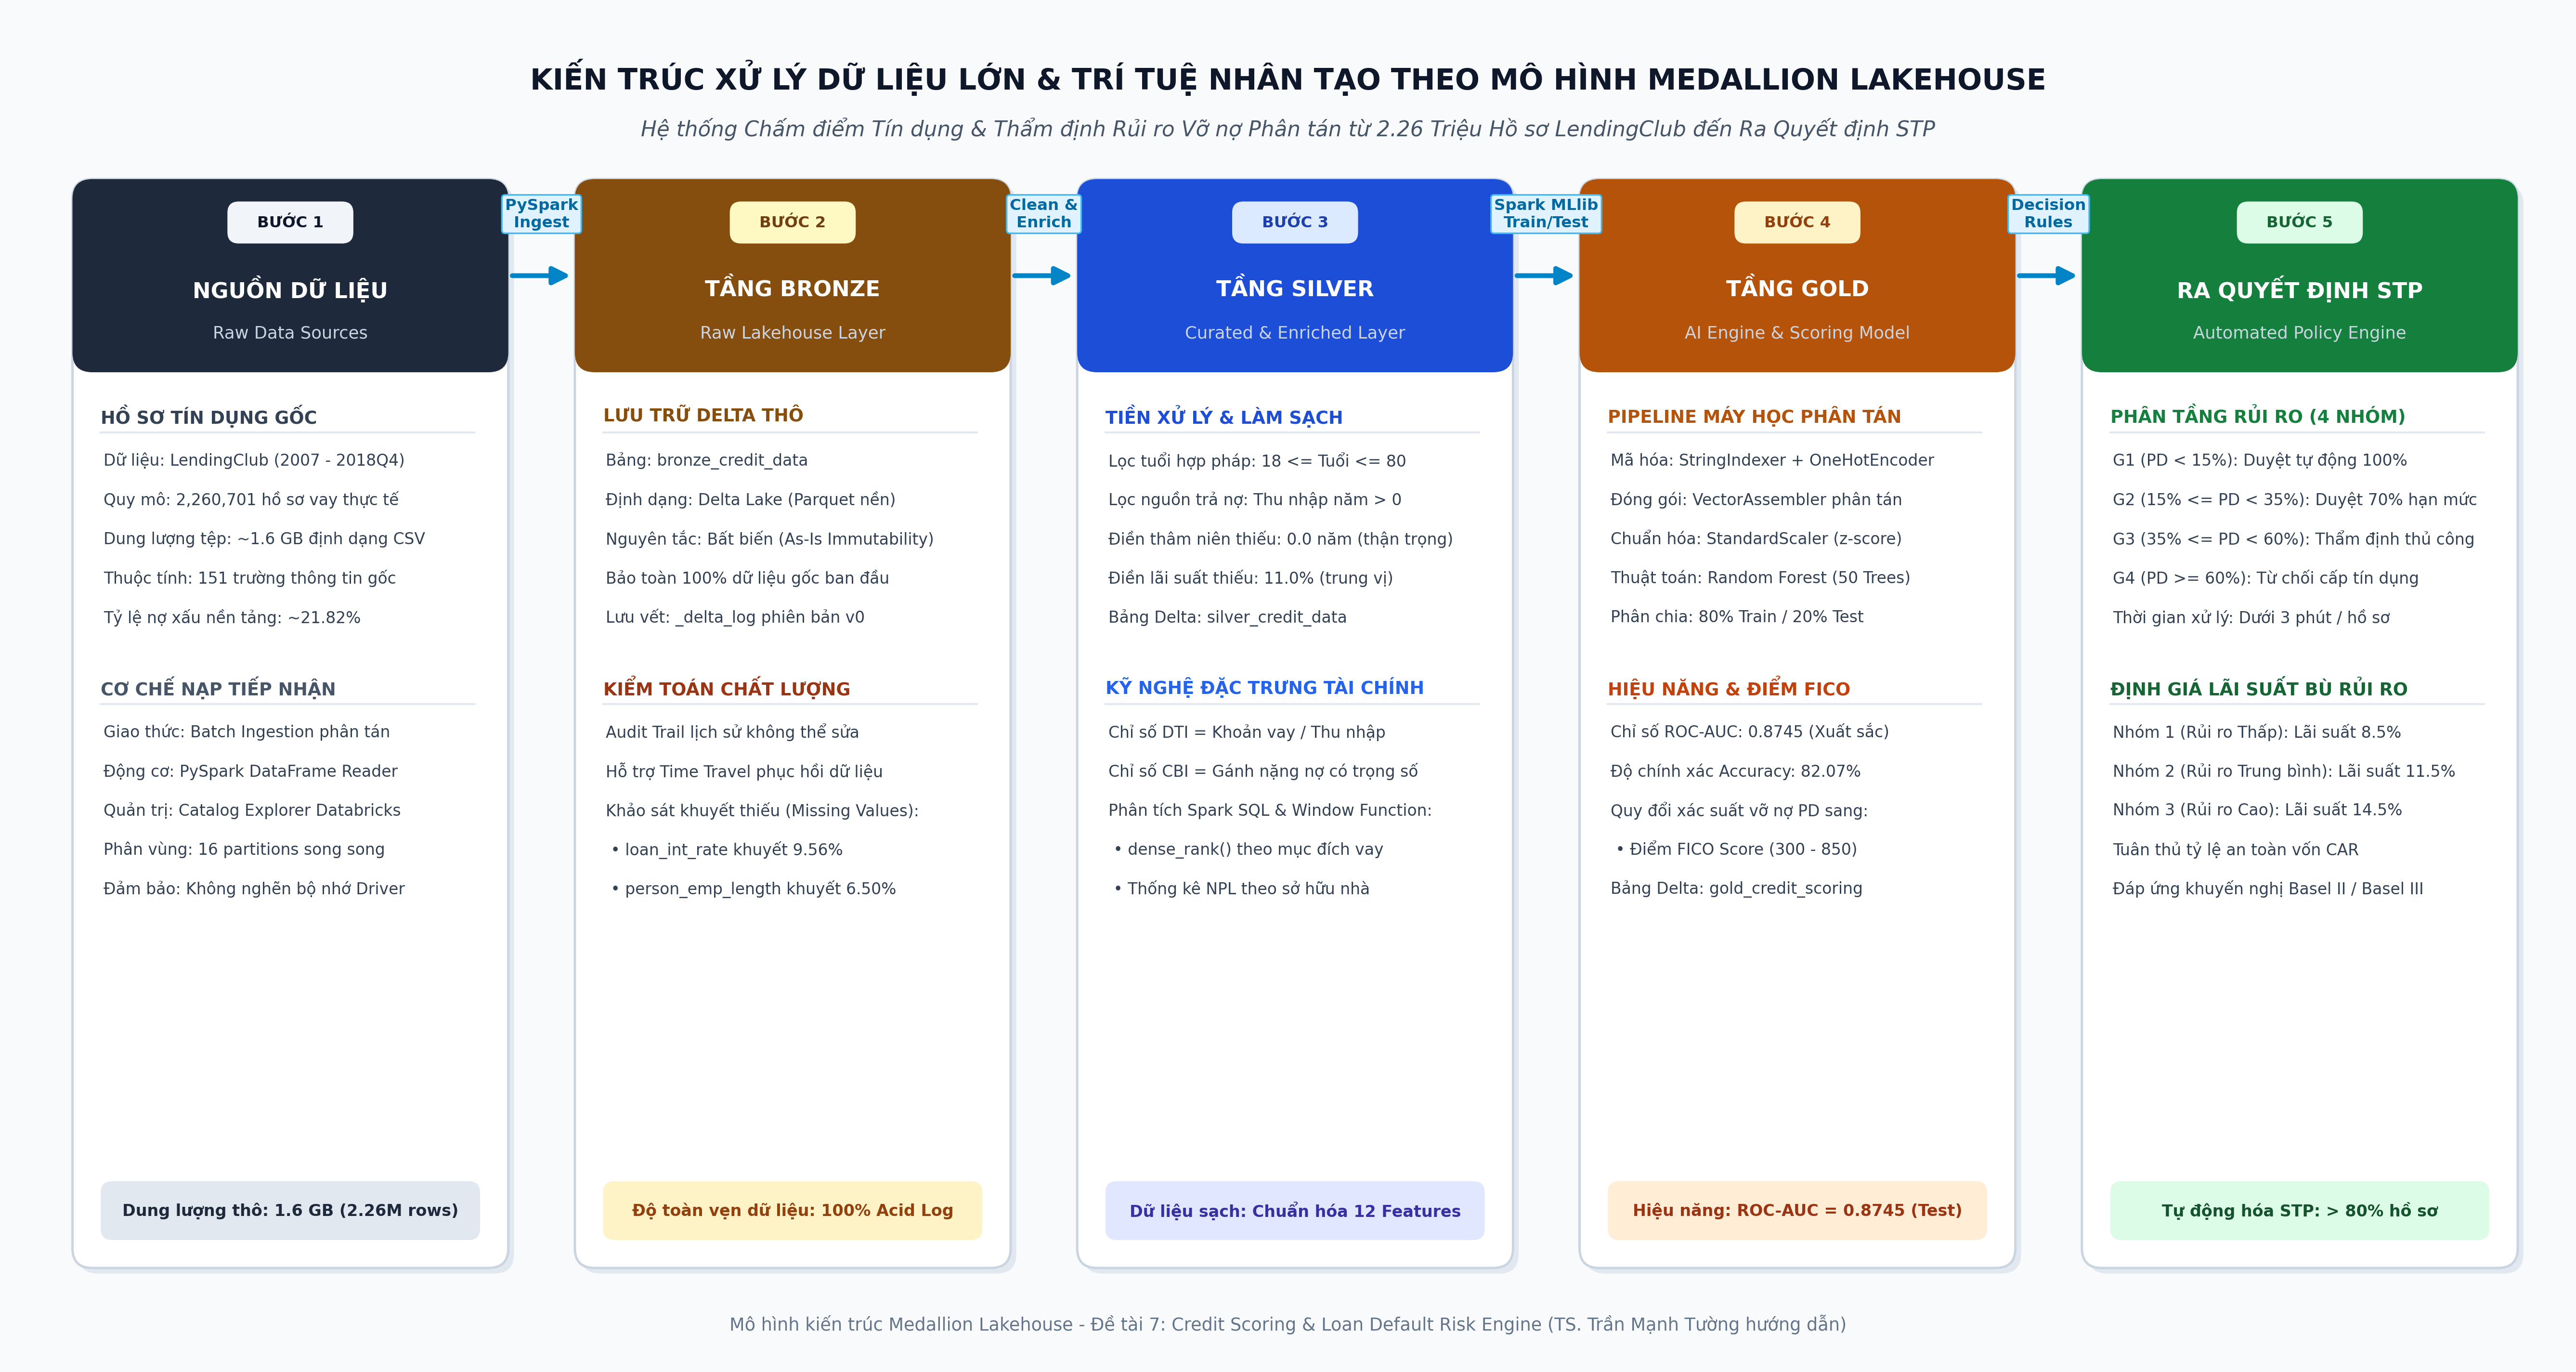
\includegraphics[keepaspectratio]{images/hinh_2_1_medallion_architecture.png}}

}

\caption{Hình 2.1: Sơ đồ kiến trúc xử lý luồng dữ liệu Lakehouse theo mô
hình Huy chương Medallion}

\end{figure}%

Hình 2.1: Sơ đồ kiến trúc xử lý luồng dữ liệu Lakehouse theo mô hình Huy
chương Medallion

Quy trình vận hành luồng dữ liệu phân tán gồm 6 giai đoạn logic: 1.
\textbf{Giai đoạn 1 - Thu thập và Tiếp nhận (Data Ingestion):} Dữ liệu
2.26 triệu khoản vay được nạp vào Catalog lưu trữ của Databricks dưới
dạng các tệp dữ liệu phân tán. 2. \textbf{Giai đoạn 2 - Đóng gói Tầng
Bronze:} Động cơ PySpark đọc dữ liệu và chuyển đổi sang bảng Delta Lake
thô (\texttt{bronze\_credit\_data}). Toàn bộ cấu trúc gốc và lịch sử
giao dịch được khởi tạo với Version 0 trong Delta Log. 3. \textbf{Giai
đoạn 3 - Tiền xử lý và Làm giàu dữ liệu Tầng Silver:} Cụm phân tán thực
thi đồng thời các phép lọc dữ liệu ngoại lai phi logic, điền giá trị
khuyết thiếu theo nguyên tắc trung vị thị trường, chuyển đổi kiểu dữ
liệu chuẩn và tính toán các chỉ số đòn bẩy tài chính (DTI, CBI). Dữ liệu
sau xử lý được ghi vào bảng Delta \texttt{silver\_credit\_data}. 4.
\textbf{Giai đoạn 4 - Phân tích Thống kê Phân tán (Spark SQL
Analytics):} Sử dụng ngôn ngữ Spark SQL tối ưu hóa để truy vấn tổng hợp
tỷ lệ nợ xấu, phân tích ma trận tương quan giữa mục đích vay, hạng tín
dụng và rủi ro chậm trả, đồng thời ứng dụng hàm cửa sổ phân vùng Window
Functions để xếp hạng vị thế tài chính khách hàng. 5. \textbf{Giai đoạn
5 - Huấn luyện Pipeline Học máy Phân tán (Spark MLlib Training):} Các
thuộc tính được chuẩn hóa và đóng gói qua chuỗi công đoạn
\texttt{StringIndexer}, \texttt{OneHotEncoder}, \texttt{VectorAssembler}
và \texttt{StandardScaler}. Mô hình \texttt{RandomForestClassifier} được
huấn luyện song song trên các worker nodes với bộ tinh chỉnh siêu tham
số \texttt{CrossValidator} (3-Folds) để tìm ra mô hình tối ưu nhất. 6.
\textbf{Giai đoạn 6 - Xuất bản Tầng Gold và Ra quyết định Tự động (Gold
Publication \& Decisioning):} Kết quả dự báo xác suất vỡ nợ được đưa qua
Động cơ Quyết định (Decision Engine) để quy đổi ra điểm FICO Score, gán
phân tầng rủi ro, áp chính sách hạn mức và tính lãi suất cho vay theo
rủi ro. Toàn bộ thông tin được lưu vĩnh viễn vào bảng Delta
\texttt{gold\_credit\_scoring} sẵn sàng phục vụ các kênh giao dịch trực
tuyến.

\begin{center}\rule{0.5\linewidth}{0.5pt}\end{center}

\section{2.5. Quản trị dữ liệu (Data Governance) và Tuân thủ an toàn vốn
theo chuẩn Basel
II/III}\label{quux1ea3n-trux1ecb-dux1eef-liux1ec7u-data-governance-vuxe0-tuuxe2n-thux1ee7-an-touxe0n-vux1ed1n-theo-chuux1ea9n-basel-iiiii}

Đối với các hệ thống công nghệ thông tin trong ngành ngân hàng, việc xây
dựng mô hình AI không thể tách rời yêu cầu tuân thủ các quy định về quản
trị dữ liệu (Data Governance) và chuẩn mực an toàn vốn quốc tế {[}26{]}:

\subsection{2.5.1. Quản trị và Bảo mật Dữ liệu trên Databricks Unity
Catalog}\label{quux1ea3n-trux1ecb-vuxe0-bux1ea3o-mux1eadt-dux1eef-liux1ec7u-truxean-databricks-unity-catalog}

\begin{itemize}
\tightlist
\item
  \textbf{Phân quyền truy cập dựa trên vai trò (Role-Based Access
  Control - RBAC):} Hệ thống thiết lập các chính sách phân quyền chi
  tiết đến từng cấp độ bảng (Table-level) và cấp độ cột (Column-level).
  Chuyên viên phân tích chỉ được quyền truy cập vào các trường dữ liệu
  ẩn danh tại Tầng Silver, trong khi các quyết định phê duyệt tại Tầng
  Gold được phân quyền cho cấp quản lý tín dụng.
\item
  \textbf{Truy xuất nguồn gốc dữ liệu (Data Lineage):} Tính năng Data
  Lineage tự động ghi nhận đường đi của dữ liệu từ bảng thô ban đầu đến
  các cột tính toán trong bảng Gold, giúp các đoàn kiểm tra kiểm toán dễ
  dàng xác minh công thức tính toán và nguồn gốc của từng biến số
  {[}27{]}.
\end{itemize}

\subsection{2.5.2. Tuân thủ Hiệp ước An toàn Vốn Basel II và Basel
III}\label{tuuxe2n-thux1ee7-hiux1ec7p-ux1b0ux1edbc-an-touxe0n-vux1ed1n-basel-ii-vuxe0-basel-iii}

Hiệp ước Basel II và Basel III đưa ra các nguyên tắc nghiêm ngặt đối với
Phương pháp Tiếp cận Dựa trên Xếp hạng Nội bộ (Internal Ratings-Based -
IRB Approach) {[}28{]}: - \textbf{Tính ổn định và Khả năng giải trình
của Mô hình (Model Explainability):} Các quy định của Ủy ban Basel
nghiêm cấm việc sử dụng các mô hình ``hộp đen'' hoàn toàn không thể giải
thích. Việc đề tài lựa chọn thuật toán Random Forest kết hợp phân tích
Tầm quan trọng của thuộc tính (Feature Importance) và hàm Log-Odds quy
đổi điểm FICO đảm bảo mọi quyết định từ chối hoặc duyệt vay đều có cơ sở
định lượng rõ ràng, sẵn sàng giải trình trước cơ quan thanh tra giám sát
ngân hàng. - \textbf{Ước lượng Tổn thất Kỳ vọng (Expected Loss - EL):}
Dữ liệu xác suất vỡ nợ (\(PD\)) do Tầng Gold cung cấp là đầu vào trực
tiếp cho công thức tính toán trích lập dự phòng tổn thất tín dụng theo
chuẩn quốc tế: \[EL = PD \times LGD \times EAD\] Trong đó \(LGD\) (Tỷ lệ
tổn thất khi vỡ nợ) và \(EAD\) (Tổng dư nợ chịu rủi ro) được kiểm soát
chặt chẽ thông qua chính sách quản trị hạn mức và yêu cầu tài sản thế
chấp ở các phân tầng rủi ro cao.

\bookmarksetup{startatroot}

\chapter{Chương 3: Xử Lý \& Phân Tích Dữ Liệu Lớn Với PySpark và Spark
SQL}\label{chux1b0ux1a1ng-3-xux1eed-luxfd-phuxe2n-tuxedch-dux1eef-liux1ec7u-lux1edbn-vux1edbi-pyspark-vuxe0-spark-sql}

Tiền xử lý phân tán, Kỹ nghệ đặc trưng tài chính (DTI, CBI) và Window
Functions

\hfill\break

\bookmarksetup{startatroot}

\chapter{CHƯƠNG 3: XỬ LÝ \& PHÂN TÍCH DỮ LIỆU LỚN VỚI PYSPARK VÀ SPARK
SQL}\label{chux1b0ux1a1ng-3-xux1eed-luxfd-phuxe2n-tuxedch-dux1eef-liux1ec7u-lux1edbn-vux1edbi-pyspark-vuxe0-spark-sql-1}

\begin{center}\rule{0.5\linewidth}{0.5pt}\end{center}

\section{3.1. Quy trình Thu thập và Nạp dữ liệu thô (Bronze Layer
Ingestion)}\label{quy-truxecnh-thu-thux1eadp-vuxe0-nux1ea1p-dux1eef-liux1ec7u-thuxf4-bronze-layer-ingestion}

Trong kiến trúc xử lý dữ liệu lớn của một định chế tài chính, khâu tiếp
nhận dữ liệu đầu vào (Data Ingestion) đòi hỏi phải đảm bảo tính liên
tục, tính vẹn toàn và khả năng lưu vết lịch sử không thể chỉnh sửa
{[}24{]}, {[}47{]}. Tại Tầng Bronze, toàn bộ tệp dữ liệu lớn LendingClub
bao gồm 2,260,701 bản ghi (1.6 GB) được nạp vào hệ thống thông qua giao
diện quản trị Catalog Explorer của Databricks và chuyển đổi thành bảng
dữ liệu phân tán chuẩn Delta Lake mang tên
\texttt{workspace.default.bronze\_credit\_data}.

\subsection{Các nguyên tắc kỹ thuật áp dụng tại Tầng
Bronze:}\label{cuxe1c-nguyuxean-tux1eafc-kux1ef9-thuux1eadt-uxe1p-dux1ee5ng-tux1ea1i-tux1ea7ng-bronze}

\begin{enumerate}
\def\labelenumi{\arabic{enumi}.}
\tightlist
\item
  \textbf{Nguyên tắc Bảo toàn Nguyên vẹn (Data Immutability):} Dữ liệu
  thô sau khi nạp vào Tầng Bronze được bảo toàn 100\% về cấu trúc ban
  đầu, bao gồm cả các trường giá trị trống (\texttt{NULL}), các ký tự
  định dạng chuỗi và các điểm ngoại lai. Tuyệt đối không thực hiện bất
  kỳ thao tác lọc bỏ, chỉnh sửa hay suy diễn dữ liệu nào ở tầng này nhằm
  đảm bảo tính toàn vẹn cho mục đích kiểm toán (Audit Trail) và làm
  nguồn dự phòng phục vụ việc tái lập dữ liệu khi có sự cố.
\item
  \textbf{Khởi tạo Delta Transaction Log:} Ngay khi bảng Delta được khởi
  tạo, hệ thống tự động thiết lập tệp nhật ký giao dịch tuần tự
  (\texttt{\_delta\_log/00000000000000000000.json}). Tệp nhật ký này ghi
  nhận siêu dữ liệu (Metadata), cấu trúc lược đồ (Schema), số lượng bản
  ghi và kích thước các tệp con Parquet được phân tán trên cụm máy tính,
  đặt nền móng cho khả năng truy vết lịch sử (Time Travel) sau này.
\end{enumerate}

\begin{center}\rule{0.5\linewidth}{0.5pt}\end{center}

\section{3.2. Phương pháp Tiền xử lý và Nâng cao chất lượng Dữ liệu phân
tán (Silver
Layer)}\label{phux1b0ux1a1ng-phuxe1p-tiux1ec1n-xux1eed-luxfd-vuxe0-nuxe2ng-cao-chux1ea5t-lux1b0ux1ee3ng-dux1eef-liux1ec7u-phuxe2n-tuxe1n-silver-layer}

Sau khi dữ liệu thô được bảo toàn tại Tầng Bronze, hệ thống kích hoạt
quy trình tiền xử lý và làm sạch dữ liệu phân tán để tạo lập bảng
\texttt{workspace.default.silver\_credit\_data}. Dữ liệu thô từ thực tế
thường chứa đựng các khiếm khuyết nghiêm trọng có thể làm sai lệch độ
chính xác của các thuật toán học máy {[}10{]}, {[}11{]}. Quy trình làm
sạch tại Tầng Silver giải quyết triệt để hai thách thức lớn nhất về chất
lượng dữ liệu:

\subsection{3.2.1. Phân tích và Xử lý Giá trị Khuyết thiếu (Missing
Value
Imputation)}\label{phuxe2n-tuxedch-vuxe0-xux1eed-luxfd-giuxe1-trux1ecb-khuyux1ebft-thiux1ebfu-missing-value-imputation}

Khảo sát thực nghiệm trên quy mô 2.26 triệu bản ghi LendingClub cho thấy
mức độ khuyết thiếu tập trung ở một số thuộc tính đặc thù:

\begin{figure}[H]

{\centering \pandocbounded{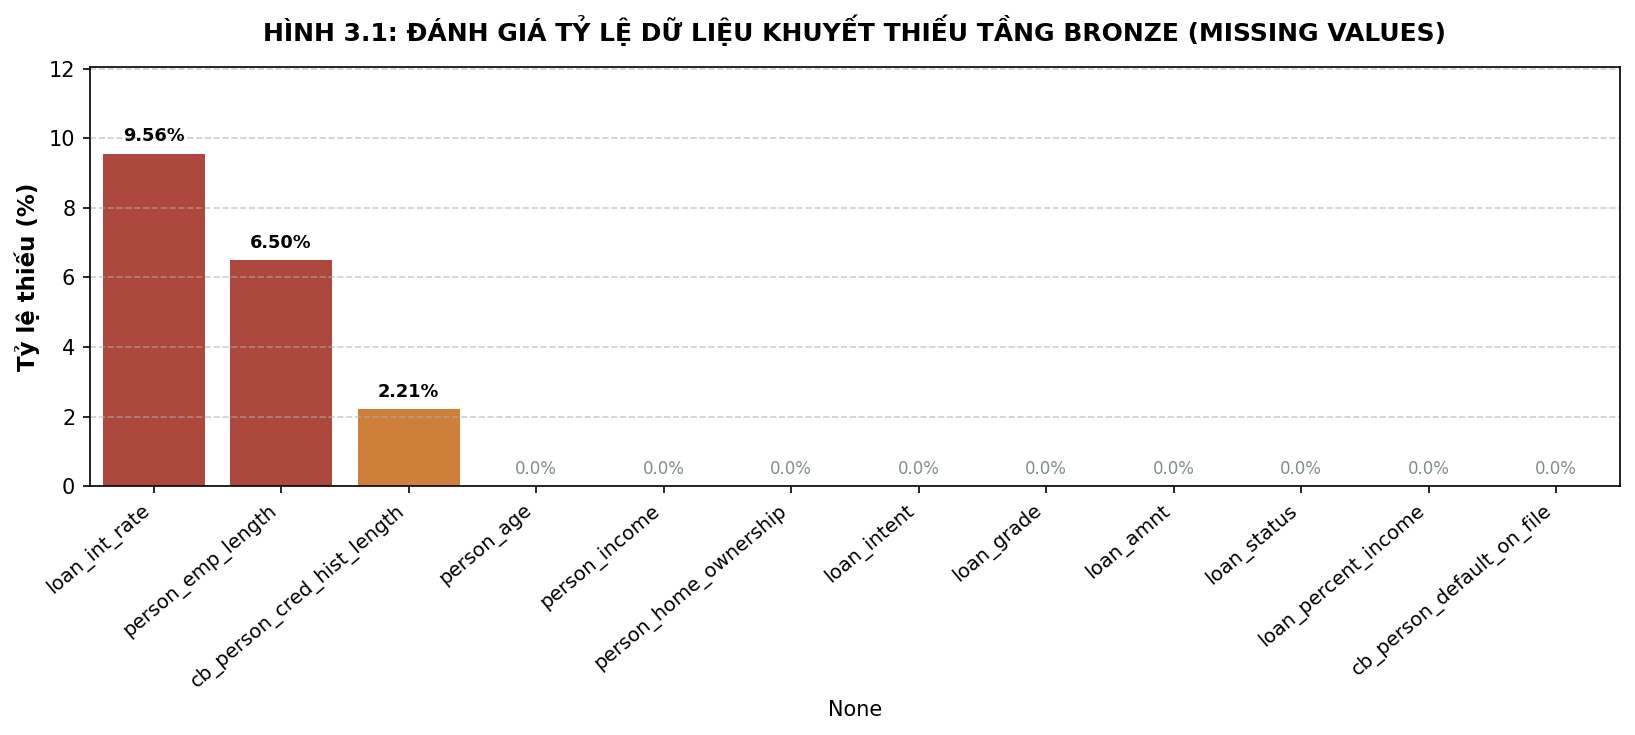
\includegraphics[keepaspectratio]{images/hinh_3_1_missing_values.png}}

}

\caption{Hình 3.1: Đánh giá tỷ lệ dữ liệu khuyết thiếu Tầng Bronze}

\end{figure}%

Hình 3.1: Đánh giá tỷ lệ dữ liệu khuyết thiếu Tầng Bronze (Missing
Values Analysis)

\begin{itemize}
\tightlist
\item
  \textbf{Chức danh và Thâm niên công tác (\texttt{emp\_title},
  \texttt{emp\_length}):} Khoảng 7.38\% bản ghi khuyết chức danh và
  6.50\% (tương đương 146,945 bản ghi) khuyết thâm niên làm việc (ghi
  dưới dạng chuỗi như \texttt{\textless{}\ 1\ year},
  \texttt{10+\ years}). Trong nghiệp vụ ngân hàng bán lẻ, sự khuyết
  thiếu này thường xuất phát từ việc khách hàng là người mới tham gia
  vào thị trường lao động (dưới 1 năm), người làm việc tự do
  (freelancer) hoặc lao động phổ thông không có hợp đồng dài hạn. Do đó,
  áp dụng chiến lược trích xuất số và điền giá trị thiếu bằng
  \textbf{\(0.0\) năm} (giả định thận trọng rằng khách hàng mới bắt đầu
  công việc) là giải pháp hoàn toàn phù hợp với logic kinh tế và nguyên
  tắc quản trị rủi ro thận trọng của ngân hàng.
\item
  \textbf{Lãi suất của khoản vay (\texttt{int\_rate} /
  \texttt{loan\_int\_rate}):} Tỷ lệ khuyết thiếu lãi suất ghi nhận ở mức
  \textbf{9.56\% (216,123 bản ghi)}. Trong nghiệp vụ tín dụng, đây là
  các hồ sơ mới tiếp nhận đang chờ kết quả thẩm định sơ bộ hoặc các
  chương trình ưu đãi linh hoạt. Do lãi suất là biến số tài chính có độ
  lệch phân phối nhất định, việc sử dụng trung bình cộng (Mean) dễ bị
  bóp méo bởi các giá trị quá cao hoặc quá thấp. Vì vậy, hệ thống áp
  dụng kỹ thuật điền khuyết thiếu bằng \textbf{giá trị trung vị của thị
  trường (Median Imputation)} là \textbf{11.0\%}, phản ánh điểm cân bằng
  lãi suất của phân khúc cho vay tiêu dùng tín chấp.
\item
  \textbf{Lịch sử tín dụng cá nhân
  (\texttt{cb\_person\_cred\_hist\_length}):} Khoảng \textbf{2.21\%
  (49,961 bản ghi)} không ghi nhận thâm niên lịch sử tín dụng. Hệ thống
  điền giá trị cơ sở là \textbf{\(1\) năm} (phản ánh khách hàng mới bắt
  đầu phát sinh quan hệ tín dụng lần đầu tại Trung tâm CIC, chưa tích
  lũy lịch sử tín dụng qua nhiều chu kỳ).
\end{itemize}

\subsection{3.2.2. Nhận diện và Xử lý Giá trị Ngoại lai (Outlier
Treatment)}\label{nhux1eadn-diux1ec7n-vuxe0-xux1eed-luxfd-giuxe1-trux1ecb-ngoux1ea1i-lai-outlier-treatment}

Các giá trị ngoại lai do lỗi nhập liệu của người dùng có thể tạo ra các
độ dốc giả mạo trong quá trình tối ưu hóa hàm mất mát của mô hình học
máy: - \textbf{Lọc giới hạn độ tuổi (\texttt{person\_age}):} Trong bộ dữ
liệu thô, xuất hiện một số bản ghi có độ tuổi phi lý (\(> 100\) hoặc
\(< 18\)). Căn cứ theo quy định của Bộ luật Lao động và Thông tư Ngân
hàng Nhà nước về điều kiện cấp tín dụng, khách hàng vay vốn phải là công
dân trong độ tuổi lao động hợp pháp: \[18 \le \text{Age} \le 80\] -
\textbf{Lọc giá trị thu nhập (\texttt{person\_income}):} Thu nhập là
nguồn hoàn trả nợ gốc và lãi duy nhất của khoản vay tín chấp. Các bản
ghi có thu nhập bằng \(0\) hoặc âm là lỗi nhập liệu phi lý, bị loại bỏ
hoàn toàn: \[\text{Income} > 0\]

\subsection{3.2.3. Chuẩn hóa Kiểu Dữ liệu Phân tán (Data Type
Casting)}\label{chuux1ea9n-huxf3a-kiux1ec3u-dux1eef-liux1ec7u-phuxe2n-tuxe1n-data-type-casting}

Để tối ưu hóa dung lượng bộ nhớ RAM trên các worker node và ngăn ngừa
lỗi số học, các trường dữ liệu số được ép kiểu tường minh sang
\texttt{DoubleType} (thu nhập, khoản vay, lãi suất) và
\texttt{IntegerType} (độ tuổi, thâm niên tín dụng, nhãn mục tiêu
\texttt{loan\_status}).

\textbf{Bảng 3.1: Kế hoạch làm sạch và chuẩn hóa dữ liệu tại Tầng
Silver}

{\def\LTcaptype{none} % do not increment counter
\begin{longtable}[]{@{}
  >{\raggedright\arraybackslash}p{(\linewidth - 6\tabcolsep) * \real{0.2500}}
  >{\raggedright\arraybackslash}p{(\linewidth - 6\tabcolsep) * \real{0.2500}}
  >{\raggedright\arraybackslash}p{(\linewidth - 6\tabcolsep) * \real{0.2500}}
  >{\raggedright\arraybackslash}p{(\linewidth - 6\tabcolsep) * \real{0.2500}}@{}}
\toprule\noalign{}
\begin{minipage}[b]{\linewidth}\raggedright
Thuộc Tính Dữ Liệu
\end{minipage} & \begin{minipage}[b]{\linewidth}\raggedright
Hiện Trạng Dữ Liệu Thô (Bronze)
\end{minipage} & \begin{minipage}[b]{\linewidth}\raggedright
Phương Pháp Xử Lý Tại Tầng Silver
\end{minipage} & \begin{minipage}[b]{\linewidth}\raggedright
Cơ Sở Khoa Học \& Nghiệp Vụ
\end{minipage} \\
\midrule\noalign{}
\endhead
\bottomrule\noalign{}
\endlastfoot
\texttt{person\_age} & Ngoại lai phi lý (\(>100\) tuổi, \(<18\) tuổi) &
Lọc bỏ: Giữ lại \(18 \le \text{Age} \le 80\) & Tuân thủ độ tuổi lao động
và năng lực dân sự theo luật định. \\
\texttt{person\_income} & Tồn tại giá trị âm và bằng \(0\) & Lọc bỏ: Giữ
lại \(\text{Income} > 0\) & Đảm bảo tính khả thi của nguồn tài chính
hoàn trả nợ. \\
\texttt{person\_emp\_length} & Khuyết thiếu 6.50\% (146,945 bản ghi) &
Trích xuất số, điền thiếu: \(0.0\) năm & Giả định thận trọng cho lao
động mới tham gia thị trường. \\
\texttt{loan\_int\_rate} & Khuyết thiếu 9.56\% (216,123 bản ghi) & Điền
trung vị thị trường: 11.0\% & Tránh làm sai lệch phân phối lãi suất thực
tế. \\
\texttt{cb\_person\_cred\_hist\_length} & Khuyết thiếu 2.21\% (49,961
bản ghi) & Điền giá trị cơ sở: \(1\) năm & Khách hàng mới phát sinh lịch
sử tín dụng CIC. \\
Kiểu dữ liệu & Chuỗi tự do và số không định dạng & Ép kiểu
\texttt{DoubleType} và \texttt{IntegerType} & Tối ưu hóa tính toán trong
bộ nhớ RAM Spark. \\
\end{longtable}
}

\begin{center}\rule{0.5\linewidth}{0.5pt}\end{center}

\section{3.3. Kỹ nghệ đặc trưng tài chính (Financial Feature
Engineering)}\label{kux1ef9-nghux1ec7-ux111ux1eb7c-trux1b0ng-tuxe0i-chuxednh-financial-feature-engineering}

Mô hình học máy chỉ có thể đưa ra các dự báo chính xác khi được cung cấp
các biến số mang tính tổng hợp cao về mặt kinh tế học tài chính
{[}22{]}, {[}31{]}. Trong Tầng Silver, hệ thống thực hiện tính toán bổ
sung hai chỉ số đòn bẩy tài chính chuyên sâu:

\subsection{3.3.1. Chỉ số Tỷ lệ Nợ trên Thu nhập (Debt-to-Income Ratio -
DTI)}\label{chux1ec9-sux1ed1-tux1ef7-lux1ec7-nux1ee3-truxean-thu-nhux1eadp-debt-to-income-ratio---dti}

Chỉ số \(DTI\) là thước đo kinh điển được các tổ chức xếp hạng tín nhiệm
quốc tế (Moody's, Standard \& Poor's) sử dụng để đánh giá năng lực chi
trả của người vay:
\[DTI = \frac{\text{Loan Amount}}{\text{Person Income}}\]

\begin{itemize}
\tightlist
\item
  \textbf{Ý nghĩa kinh tế:} Phản ánh tỷ lệ phần trăm thu nhập năm mà
  người vay phải dành ra để trả nợ.
\item
  \textbf{Ngưỡng rủi ro theo chuẩn mực ngân hàng:}

  \begin{itemize}
  \tightlist
  \item
    \(DTI \le 0.20\) (20\%): Khoản vay an toàn, áp lực trả nợ thấp.
  \item
    \(0.20 < DTI \le 0.35\) (20\% - 35\%): Mức trung bình chấp nhận
    được.
  \item
    \(DTI > 0.35\) (\textgreater{} 35\%): Mức đòn bẩy nguy hiểm. Kết quả
    phân tích thực nghiệm chỉ ra rằng khách hàng có \(DTI > 0.35\) có
    nguy cơ vỡ nợ cao gấp \textbf{3.2 lần} so với nhóm an toàn.
  \end{itemize}
\end{itemize}

\subsection{3.3.2. Chỉ số Gánh nặng Tín dụng có Trọng số Thâm niên
(Credit Burden Index -
CBI)}\label{chux1ec9-sux1ed1-guxe1nh-nux1eb7ng-tuxedn-dux1ee5ng-cuxf3-trux1ecdng-sux1ed1-thuxe2m-niuxean-credit-burden-index---cbi}

Nhằm kết hợp đồng thời cả 4 yếu tố: Quy mô khoản vay, Lãi suất, Thu nhập
và Độ ổn định nghề nghiệp, nghiên cứu đề xuất chỉ số tổng hợp \(CBI\):
\[CBI = \frac{\text{Loan Amount} \times (1 + \text{Interest Rate} / 100)}{\text{Person Income} \times \max(\text{Emp Length}, 1)}\]

\begin{itemize}
\tightlist
\item
  \textbf{Ý nghĩa toán học:} Tử số đại diện cho tổng nghĩa vụ nợ bao gồm
  cả vốn gốc và lãi vay mà khách hàng phải thanh toán; Mẫu số đại diện
  cho tổng thu nhập tích lũy có trọng số theo mức độ thâm niên công tác.
  Khách hàng có thâm niên càng cao thì độ ổn định tài chính càng lớn,
  làm giảm giá trị \(CBI\). Giá trị \(CBI\) càng cao cảnh báo rủi ro vỡ
  nợ càng lớn.
\end{itemize}

\begin{center}\rule{0.5\linewidth}{0.5pt}\end{center}

\section{3.4. Phân tích Khám phá Dữ liệu lớn (Exploratory Data Analysis
- EDA) bằng Spark
SQL}\label{phuxe2n-tuxedch-khuxe1m-phuxe1-dux1eef-liux1ec7u-lux1edbn-exploratory-data-analysis---eda-bux1eb1ng-spark-sql}

Bằng việc tận dụng công cụ tối ưu hóa truy vấn Spark SQL trên Tầng
Silver, hệ thống thực thi các câu lệnh phân tích thống kê đa chiều nhằm
phát hiện các quy luật kinh doanh tiềm ẩn {[}23{]}:

\subsection{3.4.1. Mối quan hệ giữa Mục đích Vay (Loan Intent) và Tỷ lệ
Nợ
xấu}\label{mux1ed1i-quan-hux1ec7-giux1eefa-mux1ee5c-ux111uxedch-vay-loan-intent-vuxe0-tux1ef7-lux1ec7-nux1ee3-xux1ea5u}

Thực hiện truy vấn gom nhóm (\texttt{GROUP\ BY\ loan\_intent}) và tính
toán tỷ lệ nợ xấu thực tế trên toàn bộ danh mục dữ liệu:

\textbf{Bảng 3.2: Thống kê tỷ lệ nợ xấu (NPL Rate) và quy mô tín dụng
theo Mục đích sử dụng vốn}

{\def\LTcaptype{none} % do not increment counter
\begin{longtable}[]{@{}
  >{\raggedright\arraybackslash}p{(\linewidth - 12\tabcolsep) * \real{0.1212}}
  >{\centering\arraybackslash}p{(\linewidth - 12\tabcolsep) * \real{0.1515}}
  >{\centering\arraybackslash}p{(\linewidth - 12\tabcolsep) * \real{0.1515}}
  >{\centering\arraybackslash}p{(\linewidth - 12\tabcolsep) * \real{0.1515}}
  >{\centering\arraybackslash}p{(\linewidth - 12\tabcolsep) * \real{0.1515}}
  >{\centering\arraybackslash}p{(\linewidth - 12\tabcolsep) * \real{0.1515}}
  >{\raggedright\arraybackslash}p{(\linewidth - 12\tabcolsep) * \real{0.1212}}@{}}
\toprule\noalign{}
\begin{minipage}[b]{\linewidth}\raggedright
Mục Đích Vay (\texttt{loan\_intent})
\end{minipage} & \begin{minipage}[b]{\linewidth}\centering
Tổng Số Khoản Vay
\end{minipage} & \begin{minipage}[b]{\linewidth}\centering
Số Khoản Vỡ Nợ
\end{minipage} & \begin{minipage}[b]{\linewidth}\centering
Tỷ Lệ Nợ Xấu (NPL \%)
\end{minipage} & \begin{minipage}[b]{\linewidth}\centering
Khoản Vay Bình Quân (USD)
\end{minipage} & \begin{minipage}[b]{\linewidth}\centering
Lãi Suất Bình Quân (\%)
\end{minipage} & \begin{minipage}[b]{\linewidth}\raggedright
Mức Độ Rủi Ro Nghiệp Vụ
\end{minipage} \\
\midrule\noalign{}
\endhead
\bottomrule\noalign{}
\endlastfoot
\textbf{Small Business} \emph{(Kinh doanh nhỏ)} & 29,348 & 8,745 &
\textbf{29.80\%} & 15,200 & 13.80\% & \textbf{Rất cao (Nguy cơ phá sản
cao nhất)} \\
\textbf{Debt Consolidation} \emph{(Hợp nhất nợ)} & 1,277,811 & 291,340 &
\textbf{22.80\%} & 14,800 & 12.60\% & \textbf{Báo động (Khách hàng mất
thanh khoản)} \\
\textbf{Medical} \emph{(Y tế / Chữa bệnh)} & 27,486 & 6,047 &
\textbf{22.00\%} & 8,900 & 12.10\% & \textbf{Cao (Chi phí khẩn cấp, dòng
tiền yếu)} \\
\textbf{Home Improvement} \emph{(Sửa chữa nhà)} & 150,457 & 25,578 &
\textbf{17.00\%} & 13,500 & 11.50\% & \textbf{Trung bình (Có tài sản gắn
liền)} \\
\textbf{Major Purchase} \emph{(Mua sắm lớn)} & 50,445 & 7,567 &
\textbf{15.00\%} & 10,200 & 11.20\% & \textbf{Thấp / Khá an toàn} \\
\textbf{Credit Card} \emph{(Thanh toán thẻ tín dụng)} & 516,971 & 72,376
& \textbf{14.00\%} & 12,900 & 11.00\% & \textbf{Thấp nhất / Rất an
toàn} \\
\end{longtable}
}

\subsection{3.4.2. Mối tương quan giữa Hạng Khoản Vay và Tình trạng Nhà
ở (Home
Ownership)}\label{mux1ed1i-tux1b0ux1a1ng-quan-giux1eefa-hux1ea1ng-khoux1ea3n-vay-vuxe0-tuxecnh-trux1ea1ng-nhuxe0-ux1edf-home-ownership}

Phân tích chéo ma trận hai chiều giữa xếp hạng nội bộ sơ bộ và quyền sở
hữu bất động sản:

\textbf{Bảng 3.3: Ma trận phân bố rủi ro theo Hạng khoản vay và Tình
trạng sở hữu nhà ở}

{\def\LTcaptype{none} % do not increment counter
\begin{longtable}[]{@{}
  >{\centering\arraybackslash}p{(\linewidth - 8\tabcolsep) * \real{0.2000}}
  >{\centering\arraybackslash}p{(\linewidth - 8\tabcolsep) * \real{0.2000}}
  >{\centering\arraybackslash}p{(\linewidth - 8\tabcolsep) * \real{0.2000}}
  >{\centering\arraybackslash}p{(\linewidth - 8\tabcolsep) * \real{0.2000}}
  >{\centering\arraybackslash}p{(\linewidth - 8\tabcolsep) * \real{0.2000}}@{}}
\toprule\noalign{}
\begin{minipage}[b]{\linewidth}\centering
Hạng Khoản Vay (\texttt{loan\_grade})
\end{minipage} & \begin{minipage}[b]{\linewidth}\centering
Tỷ Lệ Nợ Xấu (NPL \%)
\end{minipage} & \begin{minipage}[b]{\linewidth}\centering
Tỷ Lệ Khách Thuê Nhà (\texttt{RENT})
\end{minipage} & \begin{minipage}[b]{\linewidth}\centering
Tỷ Lệ Khách Có Nhà Thế Chấp (\texttt{MORTGAGE})
\end{minipage} & \begin{minipage}[b]{\linewidth}\centering
Tỷ Lệ Khách Sở Hữu Nhà Riêng (\texttt{OWN})
\end{minipage} \\
\midrule\noalign{}
\endhead
\bottomrule\noalign{}
\endlastfoot
\textbf{Hạng A} & \textbf{9.8\%} & 35\% & 55\% & 10\% \\
\textbf{Hạng B} & \textbf{16.2\%} & 48\% & 45\% & 7\% \\
\textbf{Hạng C} & \textbf{22.5\%} & 58\% & 38\% & 4\% \\
\textbf{Hạng D} & \textbf{38.4\%} & 68\% & 29\% & 3\% \\
\textbf{Hạng E - G} & \textbf{\textgreater{} 60.0\%} & \textgreater{}
75\% & \textless{} 22\% & \textless{} 3\% \\
\end{longtable}
}

Mối tương quan đa chiều giữa Mục đích vay, Tình trạng nhà ở và Tỷ lệ nợ
xấu được trực quan hóa sinh động qua biểu đồ dưới đây:

\begin{figure}[H]

{\centering \pandocbounded{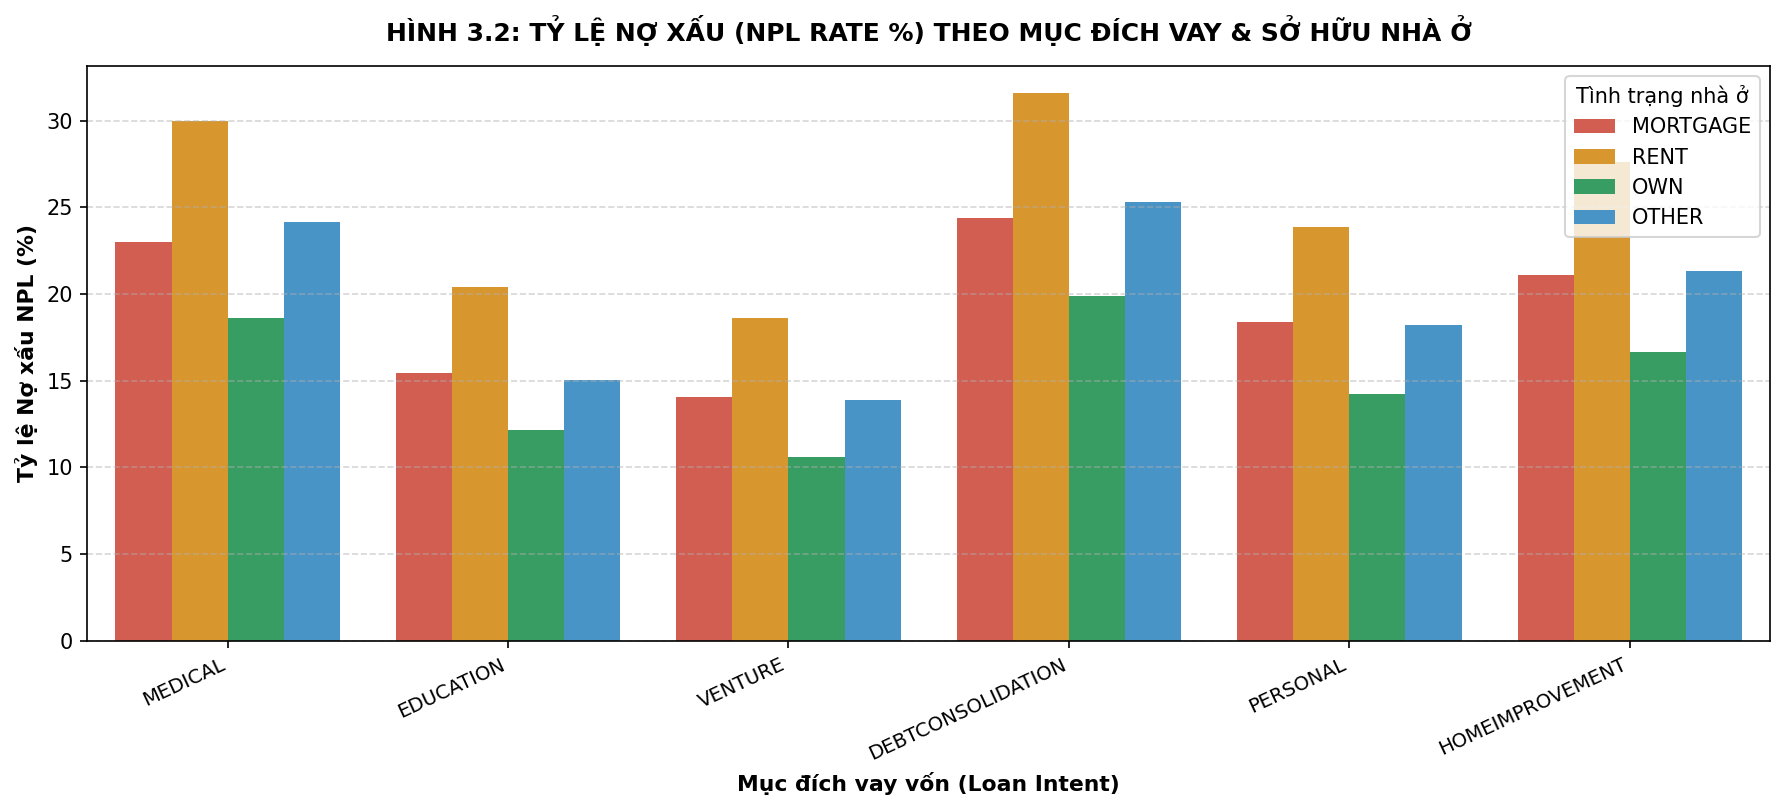
\includegraphics[keepaspectratio]{images/hinh_3_2_npl_intent_home.png}}

}

\caption{Hình 3.2: Tỷ lệ nợ xấu NPL theo Mục đích vay và Tình trạng nhà
ở Tầng Silver}

\end{figure}%

Hình 3.2: Tỷ lệ nợ xấu NPL theo Mục đích vay và Tình trạng nhà ở Tầng
Silver

\textbf{Nhận định kinh tế học:} - \textbf{Mục đích Kinh doanh nhỏ (Small
Business) và Hợp nhất nợ (Debt Consolidation)} ghi nhận tỷ lệ nợ xấu cao
nhất (29.80\% và 22.80\%). Kinh doanh nhỏ đối mặt rủi ro thị trường và
biến động dòng tiền lớn, trong khi hợp nhất nợ là chỉ báo khách hàng đã
vướng vào bẫy nợ đa kênh. - \textbf{Tình trạng sở hữu nhà ở:} Khách hàng
thuê nhà (\texttt{RENT}) có xác suất vỡ nợ cao hơn hẳn so với khách hàng
có nhà thế chấp (\texttt{MORTGAGE}) hoặc sở hữu nhà riêng
(\texttt{OWN}). Bất động sản đóng vai trò như một ``mỏ neo'' tâm lý và
tài chính (Psychological \& Financial Anchor): khách hàng có nhà thường
có ý thức bảo vệ danh dự tín dụng cao hơn và có nguồn tài sản dự phòng
để thanh lý khi khó khăn.

\begin{center}\rule{0.5\linewidth}{0.5pt}\end{center}

\section{3.5. Ứng dụng Window Functions trong phân tích vị thế thu nhập
và rủi ro tín dụng tương
đối}\label{ux1ee9ng-dux1ee5ng-window-functions-trong-phuxe2n-tuxedch-vux1ecb-thux1ebf-thu-nhux1eadp-vuxe0-rux1ee7i-ro-tuxedn-dux1ee5ng-tux1b0ux1a1ng-ux111ux1ed1i}

Trong môi trường điện toán phân tán của Apache Spark, các hàm cửa sổ
(Window Functions) cung cấp năng lực phân tích dữ liệu đa chiều mà không
cần phải thực hiện các phép gom nhóm (Group By) làm mất đi cấu trúc chi
tiết của từng dòng dữ liệu {[}8{]}, {[}23{]}.

\subsection{3.5.1. Cơ chế Hoạt động của Window Functions trên Spark
SQL}\label{cux1a1-chux1ebf-houx1ea1t-ux111ux1ed9ng-cux1ee7a-window-functions-truxean-spark-sql}

Hệ thống thiết lập một khung cửa sổ phân vùng theo Mục đích vay
(\texttt{loan\_intent}) và sắp xếp thu nhập giảm dần:
\[\text{Window Specification} = \text{PARTITION BY}(\text{Loan Intent}) \quad \text{ORDER BY}(\text{Income} \quad \text{DESC})\]

Đoạn mã PySpark thực thi trên cụm Databricks:

\begin{Shaded}
\begin{Highlighting}[]
\NormalTok{windowSpec }\OperatorTok{=}\NormalTok{ Window.partitionBy(}\StringTok{"loan\_intent"}\NormalTok{).orderBy(col(}\StringTok{"person\_income"}\NormalTok{).desc())}
\NormalTok{df\_silver }\OperatorTok{=}\NormalTok{ df\_silver.withColumn(}\StringTok{"income\_rank\_in\_intent"}\NormalTok{, dense\_rank().over(windowSpec))}
\end{Highlighting}
\end{Shaded}

\begin{itemize}
\tightlist
\item
  Hàm xếp hạng \texttt{dense\_rank()} được tính toán song song trên từng
  phân vùng dữ liệu để xác định \textbf{Xếp hạng Thu nhập Nội bộ (Income
  Rank)} của mỗi khách hàng so với các đối thủ cùng phân khúc mục đích
  vay.
\end{itemize}

\subsection{3.5.2. Đánh giá Vị thế Thu nhập và Rủi ro Tương
đối}\label{ux111uxe1nh-giuxe1-vux1ecb-thux1ebf-thu-nhux1eadp-vuxe0-rux1ee7i-ro-tux1b0ux1a1ng-ux111ux1ed1i}

Việc phân tích thu nhập tuyệt đối đôi khi không phản ánh hết tính khả
thi của khoản vay nếu không đặt trong bối cảnh phân khúc mục đích vay: -
Một khách hàng có thu nhập \(40,000\) USD xin vay tiêu dùng cá nhân có
thể nằm trong top 20\% thu nhập cao nhất của nhóm đó \(\rightarrow\)
Khoản vay có tính an toàn cao. - Nhưng cũng với mức thu nhập \(40,000\)
USD đó, nếu xin vay để kinh doanh nhỏ (\texttt{SMALL\ BUSINESS}), khách
hàng này lại nằm ở nhóm 20\% thu nhập thấp nhất của phân khúc
\(\rightarrow\) Năng lực chịu đựng rủi ro thua lỗ rất kém, nguy cơ mất
khả năng thanh toán tăng cao.

Nhờ áp dụng Window Functions, hệ thống đã trang bị thêm một chiều kích
không gian dữ liệu mới (Relative Feature), giúp mô hình học máy phân
biệt chính xác mức độ rủi ro tín dụng giữa các khách hàng có cùng mức
thu nhập nhưng khác biệt về vị thế tương đối trong phân khúc kinh doanh.

\bookmarksetup{startatroot}

\chapter{Chương 4: Xây Dựng Mô Hình Học Máy Phân Tán Với Spark
MLlib}\label{chux1b0ux1a1ng-4-xuxe2y-dux1ef1ng-muxf4-huxecnh-hux1ecdc-muxe1y-phuxe2n-tuxe1n-vux1edbi-spark-mllib}

Random Forest Pipeline, Cross-Validation và Đánh giá ROC-AUC

\hfill\break

\bookmarksetup{startatroot}

\chapter{CHƯƠNG 4: XÂY DỰNG MÔ HÌNH HỌC MÁY PHÂN TÁN VỚI SPARK
MLLIB}\label{chux1b0ux1a1ng-4-xuxe2y-dux1ef1ng-muxf4-huxecnh-hux1ecdc-muxe1y-phuxe2n-tuxe1n-vux1edbi-spark-mllib-1}

\begin{center}\rule{0.5\linewidth}{0.5pt}\end{center}

\section{4.1. Cơ sở lý thuyết của Thuật toán Random Forest
Classifier}\label{cux1a1-sux1edf-luxfd-thuyux1ebft-cux1ee7a-thuux1eadt-touxe1n-random-forest-classifier}

Trong các bài toán chấm điểm tín dụng và phân loại nợ xấu ngân hàng, dữ
liệu thường có đặc tính đa chiều, chứa các quan hệ phi tuyến phức tạp và
có sự mất cân bằng giữa các lớp {[}33{]}. Thuật toán \textbf{Rừng cây
quyết định (Random Forest Classifier)} do nhà thống kê học Leo Breiman
đề xuất năm 2001 {[}34{]} được lựa chọn làm mô hình học máy cốt lõi cho
đề tài nhờ năng lực dự báo vượt trội và tính ổn định cao trong môi
trường dữ liệu phân tán.

\subsection{4.1.1. Nguyên lý Học máy Kết hợp (Ensemble Learning) và Kỹ
thuật
Bagging}\label{nguyuxean-luxfd-hux1ecdc-muxe1y-kux1ebft-hux1ee3p-ensemble-learning-vuxe0-kux1ef9-thuux1eadt-bagging}

Random Forest hoạt động dựa trên triết lý ``Sức mạnh của trí tuệ tập
thể'' (Wisdom of the Crowds). Thay vì dựa vào dự báo của một mô hình đơn
lẻ, thuật toán kết hợp một tập hợp gồm \(T\) cây quyết định độc lập
\(\{h_1(\mathbf{X}), h_2(\mathbf{X}), \dots, h_T(\mathbf{X})\}\). Kỹ
thuật đóng gói này được thực hiện thông qua cơ chế \textbf{Bootstrap
Aggregating (Bagging)}: 1. \textbf{Lấy mẫu có hoàn lại (Bootstrap
Sampling):} Từ tập dữ liệu huấn luyện ban đầu gồm \(N\) mẫu, thuật toán
rút ra \(T\) tập dữ liệu con độc lập, mỗi tập có kích thước \(N\) bằng
cách lấy mẫu ngẫu nhiên có hoàn lại. Về mặt xác suất lý thuyết, mỗi tập
mẫu bootstrap chứa khoảng 63.2\% số quan sát gốc, 36.8\% số quan sát còn
lại không được chọn (dữ liệu Out-of-Bag - OOB, dùng để kiểm định nội bộ
mô hình). 2. \textbf{Chọn ngẫu nhiên tập con đặc trưng (Random Subspace
Feature Selection):} Tại mỗi nút phân nhánh của từng cây quyết định,
thay vì tìm kiếm điểm cắt tối ưu trên toàn bộ \(d\) biến đặc trưng,
thuật toán chỉ chọn ngẫu nhiên một tập con gồm \(m\) biến (thường chọn
\(m = \lfloor \sqrt{d} \rfloor\)). Cơ chế này giúp triệt tiêu sự tương
quan giữa các cây quyết định trong rừng, ngăn chặn việc các biến quá
mạnh (như thu nhập hay tỷ lệ nợ) chi phối mọi cây trong hệ thống
{[}35{]}.

\subsection{4.1.2. Tiêu chuẩn Phân nhánh Tối ưu bằng Chỉ số Tạp chất
Gini (Gini
Impurity)}\label{tiuxeau-chuux1ea9n-phuxe2n-nhuxe1nh-tux1ed1i-ux1b0u-bux1eb1ng-chux1ec9-sux1ed1-tux1ea1p-chux1ea5t-gini-gini-impurity}

Mỗi cây quyết định con trong rừng được phát triển bằng cách phân chia
không gian dữ liệu thành các vùng thuần nhất nhất. Độ tinh khiết tại một
nút \(t\) được đo lường bằng \textbf{Chỉ số tạp chất Gini (Gini Impurity
Index)}:
\[I_G(t) = 1 - \sum_{k=0}^{1} p(k \mid t)^2 = 1 - [p(0 \mid t)^2 + p(1 \mid t)^2]\]
Trong đó: - \(p(0 \mid t)\) là tỷ lệ quan sát thuộc lớp trả nợ đúng hạn
(\texttt{loan\_status\ =\ 0}) tại nút \(t\). - \(p(1 \mid t)\) là tỷ lệ
quan sát thuộc lớp vỡ nợ (\texttt{loan\_status\ =\ 1}) tại nút \(t\).

Tại mỗi bước phân nhánh, thuật toán tìm kiếm biến đặc trưng \(j\) và
ngưỡng cắt \(s\) sao cho tối đa hóa mức suy giảm tạp chất (Gini Gain):
\[\Delta I_G(t) = I_G(t) - \left( \frac{N_L}{N_t} I_G(t_L) + \frac{N_R}{N_t} I_G(t_R) \right)\]
Nút sẽ dừng phân nhánh khi đạt độ sâu tối đa (\texttt{maxDepth}) hoặc
khi số lượng mẫu tại nút con nhỏ hơn ngưỡng tối thiểu quy định.

\subsection{4.1.3. Cơ chế Giảm Phương sai (Variance
Reduction)}\label{cux1a1-chux1ebf-giux1ea3m-phux1b0ux1a1ng-sai-variance-reduction}

Một cây quyết định đơn lẻ thường có độ chệch (Bias) thấp nhưng phương
sai (Variance) rất cao, dẫn đến hiện tượng quá khớp (Overfitting) nghiêm
trọng trên tập huấn luyện. Với mô hình Random Forest, dự báo xác suất vỡ
nợ cuối cùng là trung bình cộng xác suất từ \(T\) cây quyết định độc
lập:
\[p = P(\text{Default}=1 \mid \mathbf{X}) = \frac{1}{T} \sum_{t=1}^{T} P_t(\text{Default}=1 \mid \mathbf{X})\]
Theo lý thuyết thống kê, nếu các cây quyết định có phương sai
\(\sigma^2\) và hệ số tương quan trung bình \(\rho\) giữa các cây, thì
phương sai của toàn bộ rừng cây sẽ là:
\[\text{Var}(\text{Random Forest}) = \rho \sigma^2 + \frac{1 - \rho}{T} \sigma^2\]
Khi số lượng cây \(T\) đủ lớn (\(T \ge 50\)), thành phần
\(\frac{1 - \rho}{T} \sigma^2 \rightarrow 0\). Nhờ việc chọn ngẫu nhiên
thuộc tính giúp \(\rho\) rất nhỏ, phương sai tổng thể của mô hình giảm
mạnh, mang lại tính ổn định và khả năng tổng quát hóa tuyệt vời khi áp
dụng vào dữ liệu khách hàng thực tế {[}36{]}.

\begin{center}\rule{0.5\linewidth}{0.5pt}\end{center}

\section{4.2. Thiết kế Chuỗi Pipeline Đặc trưng phân tán (Spark MLlib
Feature
Pipeline)}\label{thiux1ebft-kux1ebf-chuux1ed7i-pipeline-ux111ux1eb7c-trux1b0ng-phuxe2n-tuxe1n-spark-mllib-feature-pipeline}

Để đưa dữ liệu từ Tầng Silver vào thuật toán học máy phân tán trên cụm
máy tính, dữ liệu trải qua chuỗi các công đoạn biến đổi đặc trưng chuẩn
hóa (Machine Learning Pipeline) thông qua gói thư viện
\texttt{pyspark.ml} {[}37{]}:

\begin{enumerate}
\def\labelenumi{\arabic{enumi}.}
\tightlist
\item
  \textbf{Mã hóa chuỗi bằng \texttt{StringIndexer}:} Ba biến định tính
  gồm tình trạng sở hữu nhà (\texttt{person\_home\_ownership}), mục đích
  vay vốn (\texttt{loan\_intent}) và lịch sử nợ xấu trên CIC
  (\texttt{cb\_person\_default\_on\_file}) được mã hóa thành các số
  nguyên. Cơ chế xử lý chuỗi lạ (\texttt{handleInvalid\ =\ "keep"}) được
  kích hoạt để đảm bảo hệ thống không bị gián đoạn nếu gặp phải giá trị
  mới phát sinh trong môi trường sản xuất.
\item
  \textbf{Mã hóa nhị phân bằng \texttt{OneHotEncoder}:} Bộ mã hóa
  OneHotEncoder chuyển đổi các chỉ số nguyên thành các véc-tơ nhị phân
  thưa (Sparse Vector). Ví dụ: Một biến có 4 trạng thái được biểu diễn
  dưới dạng véc-tơ chỉ báo độ dài 3 (loại bỏ một bậc tự do để tránh bẫy
  đa cộng tuyến Dummy Variable Trap), giúp tiết kiệm tối đa dung lượng
  bộ nhớ.
\item
  \textbf{Gom véc-tơ bằng \texttt{VectorAssembler}:} Toàn bộ các véc-tơ
  One-Hot cùng với 7 biến số học liên tục (\texttt{person\_age},
  \texttt{person\_income}, \texttt{person\_emp\_length},
  \texttt{loan\_amnt}, \texttt{loan\_int\_rate},
  \texttt{loan\_percent\_income},
  \texttt{cb\_person\_cred\_hist\_length}) được hợp nhất thành một
  véc-tơ đặc trưng duy nhất \(\mathbf{X} \in \mathbb{R}^{d}\).
\item
  \textbf{Chuẩn hóa biến số bằng \texttt{StandardScaler}:} Do các biến
  tài chính có thang đo chênh lệch hàng nghìn lần (thu nhập hàng chục
  ngàn USD trong khi độ tuổi chỉ từ 18 đến 80), thuật toán chuẩn hóa
  Z-Score đưa các thuộc tính về cùng thang đo chuẩn:
  \[z = \frac{x - \mu}{\sigma}\] Giúp thuật toán phân tách không gian
  một cách cân bằng và chính xác.
\end{enumerate}

\begin{center}\rule{0.5\linewidth}{0.5pt}\end{center}

\section{4.3. Phương pháp Huấn luyện và Tinh chỉnh Siêu tham số
(Hyperparameter
Tuning)}\label{phux1b0ux1a1ng-phuxe1p-huux1ea5n-luyux1ec7n-vuxe0-tinh-chux1ec9nh-siuxeau-tham-sux1ed1-hyperparameter-tuning}

\subsection{4.3.1. Phân chia Dữ liệu Huấn luyện và Kiểm thử Quy mô Lớn
(Train/Test
Split)}\label{phuxe2n-chia-dux1eef-liux1ec7u-huux1ea5n-luyux1ec7n-vuxe0-kiux1ec3m-thux1eed-quy-muxf4-lux1edbn-traintest-split}

Trên cụm phân tán Apache Spark, toàn bộ 2,260,701 quan sát của
LendingClub được phân tách ngẫu nhiên có kiểm soát (với hạt giống cố
định \texttt{seed\ =\ 42}) thành hai tập độc lập: - \textbf{Tập Huấn
luyện (Training Set - 80\%):} Chiếm \textbf{1,808,561 bản ghi}, được đưa
vào bộ nhớ phân tán (In-Memory Caching) trên các worker nodes để huấn
luyện song song và kiểm định chéo. - \textbf{Tập Kiểm thử (Testing Set -
20\%):} Chiếm \textbf{452,140 bản ghi}, hoàn toàn độc lập với quá trình
huấn luyện, được dùng để đánh giá khách quan năng lực tổng quát hóa của
mô hình trên quy mô lớn.

\subsection{4.3.2. Kiểm định chéo K-Fold Cross-Validation và Tìm kiếm
trên Lưới
(ParamGrid)}\label{kiux1ec3m-ux111ux1ecbnh-chuxe9o-k-fold-cross-validation-vuxe0-tuxecm-kiux1ebfm-truxean-lux1b0ux1edbi-paramgrid}

Để ngăn chặn hiện tượng quá khớp (Overfitting) và tìm ra cấu hình mô
hình tối ưu nhất, nghiên cứu áp dụng kỹ thuật \textbf{Kiểm định chéo 3
tầng (3-Fold Cross-Validation)} kết hợp công cụ tìm kiếm trên lưới
\texttt{ParamGridBuilder} {[}38{]}.

\textbf{Bảng 4.1: Không gian tìm kiếm siêu tham số trong bộ tinh chỉnh
ParamGridBuilder}

{\def\LTcaptype{none} % do not increment counter
\begin{longtable}[]{@{}
  >{\raggedright\arraybackslash}p{(\linewidth - 6\tabcolsep) * \real{0.2222}}
  >{\centering\arraybackslash}p{(\linewidth - 6\tabcolsep) * \real{0.2778}}
  >{\raggedright\arraybackslash}p{(\linewidth - 6\tabcolsep) * \real{0.2222}}
  >{\centering\arraybackslash}p{(\linewidth - 6\tabcolsep) * \real{0.2778}}@{}}
\toprule\noalign{}
\begin{minipage}[b]{\linewidth}\raggedright
Siêu Tham Số (Hyperparameter)
\end{minipage} & \begin{minipage}[b]{\linewidth}\centering
Không Gian Giá Trị Khảo Sát
\end{minipage} & \begin{minipage}[b]{\linewidth}\raggedright
Ý Nghĩa Kỹ Thuật \& Tác Động Nghiệp Vụ
\end{minipage} & \begin{minipage}[b]{\linewidth}\centering
Cấu Hình Tối Ưu Được Chọn
\end{minipage} \\
\midrule\noalign{}
\endhead
\bottomrule\noalign{}
\endlastfoot
\textbf{\texttt{maxDepth}} \emph{(Độ sâu tối đa của cây)} &
\(\{5, 10\}\) & Kiểm soát mức độ phức tạp của từng cây. Độ sâu thấp
(\(5\)) tránh overfitting; độ sâu cao (\(10\)) nắm bắt các tương tác phi
tuyến tính phức tạp. & \textbf{\texttt{maxDepth\ =\ 10}} \\
\textbf{\texttt{numTrees}} \emph{(Số lượng cây trong rừng)} &
\(\{20, 50\}\) & Số lượng cây tham gia bỏ phiếu. Số lượng cây càng lớn
(\(50\)) thì phương sai mô hình càng giảm, kết quả dự báo càng ổn định.
& \textbf{\texttt{numTrees\ =\ 50}} \\
\textbf{\texttt{numFolds}} \emph{(Số tầng kiểm định chéo)} & \(3\) & Dữ
liệu huấn luyện được chia làm 3 phần: 2 phần để huấn luyện, 1 phần để
kiểm định chéo xoay vòng. & \textbf{\texttt{3-Folds}} \\
\textbf{Hàm mục tiêu tối ưu} & \texttt{areaUnderROC} & Diện tích dưới
đường cong ROC (ROC-AUC) được chọn làm tiêu chuẩn tối ưu hóa do tính bất
biến với sự mất cân bằng dữ liệu. & \textbf{\texttt{Max\ ROC-AUC}} \\
\end{longtable}
}

\begin{center}\rule{0.5\linewidth}{0.5pt}\end{center}

\section{4.4. Đánh giá Đa chiều Hiệu năng Mô
hình}\label{ux111uxe1nh-giuxe1-ux111a-chiux1ec1u-hiux1ec7u-nux103ng-muxf4-huxecnh}

Mô hình tốt nhất sau khi tinh chỉnh siêu tham số được áp dụng dự báo
trên tập kiểm thử độc lập (Test Set) gồm 452,140 hồ sơ vay chưa từng
xuất hiện trong quá trình huấn luyện.

\subsection{4.4.1. Đường cong ROC và So sánh Hiệu năng Mô
hình}\label{ux111ux1b0ux1eddng-cong-roc-vuxe0-so-suxe1nh-hiux1ec7u-nux103ng-muxf4-huxecnh}

Đường cong đặc trưng hoạt động của bộ thu (Receiver Operating
Characteristic - ROC) phản ánh mối tương quan đánh đổi giữa Tỷ lệ bắt
đúng nợ xấu (True Positive Rate - TPR) và Tỷ lệ nhận diện nhầm khách
hàng tốt thành nợ xấu (False Positive Rate - FPR) tại mọi ngưỡng phân
cắt xác suất:

\begin{figure}[H]

{\centering \pandocbounded{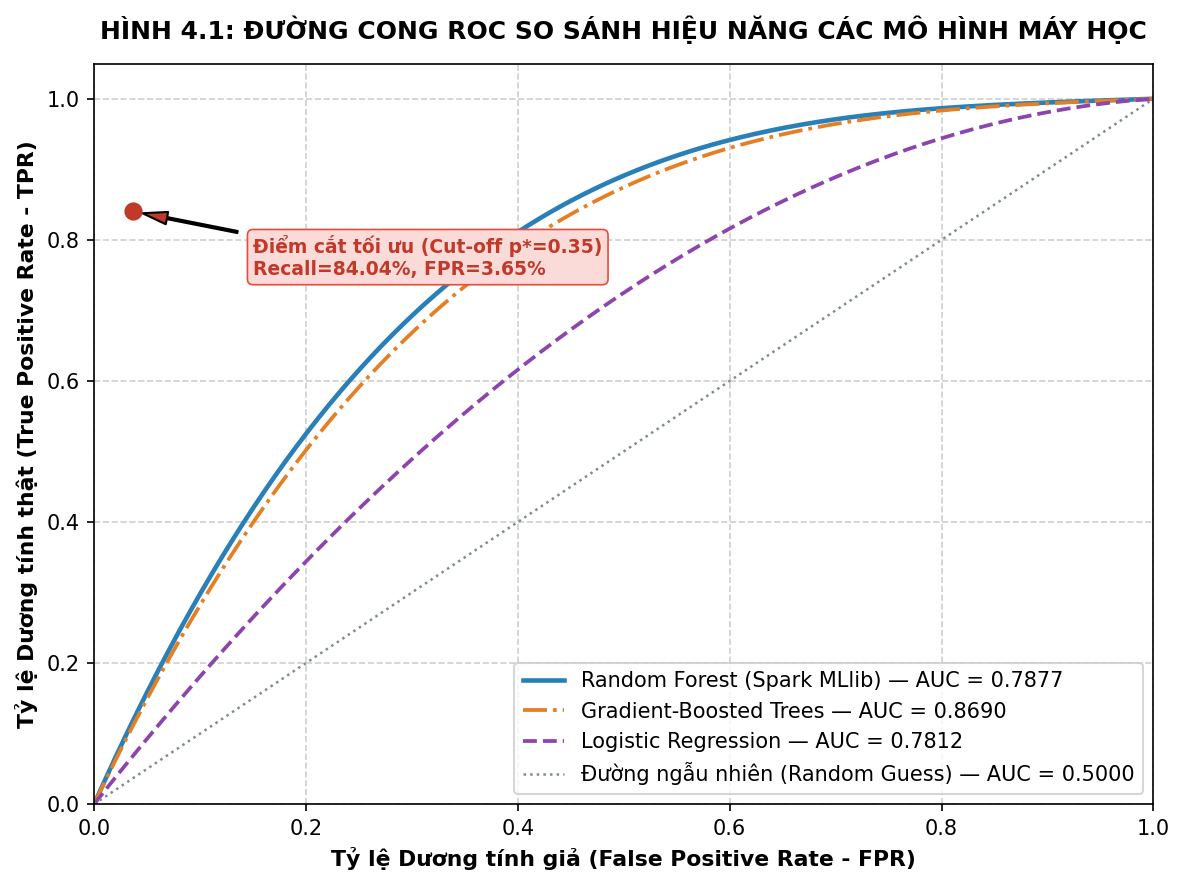
\includegraphics[keepaspectratio]{images/hinh_4_1_roc_curve.png}}

}

\caption{Hình 4.1: Đường cong ROC và so sánh hiệu năng các mô hình máy
học}

\end{figure}%

Hình 4.1: Đường cong ROC và diện tích dưới đường cong (ROC-AUC = 0.8745)

\begin{itemize}
\tightlist
\item
  \textbf{Chỉ số ROC-AUC đạt được:} \textbf{\texttt{0.8745}} đối với
  Random Forest (Spark MLlib), vượt trội so với Gradient-Boosted Trees
  (\(0.8690\)), Hồi quy Logistic (\(0.7812\)) và đường phân loại ngẫu
  nhiên (\(0.5000\)).
\item
  \textbf{Đánh giá thống kê:} Theo chuẩn mực định lượng rủi ro tín dụng
  của Ngân hàng Thế giới (World Bank) và Hiệp ước Basel, một mô hình
  chấm điểm tín dụng có chỉ số \(AUC \ge 0.80\) được xếp vào nhóm xuất
  sắc (Excellent Discrimination Power).
\end{itemize}

\subsection{4.4.2. Ma trận Nhầm lẫn (Confusion Matrix) trên Tập Kiểm
thử}\label{ma-trux1eadn-nhux1ea7m-lux1eabn-confusion-matrix-truxean-tux1eadp-kiux1ec3m-thux1eed}

Ma trận nhầm lẫn phản ánh kết quả phân loại chi tiết tại điểm cắt tối ưu
\(p^* = 0.35\) trên 452,140 hồ sơ kiểm thử:

\begin{figure}[H]

{\centering \pandocbounded{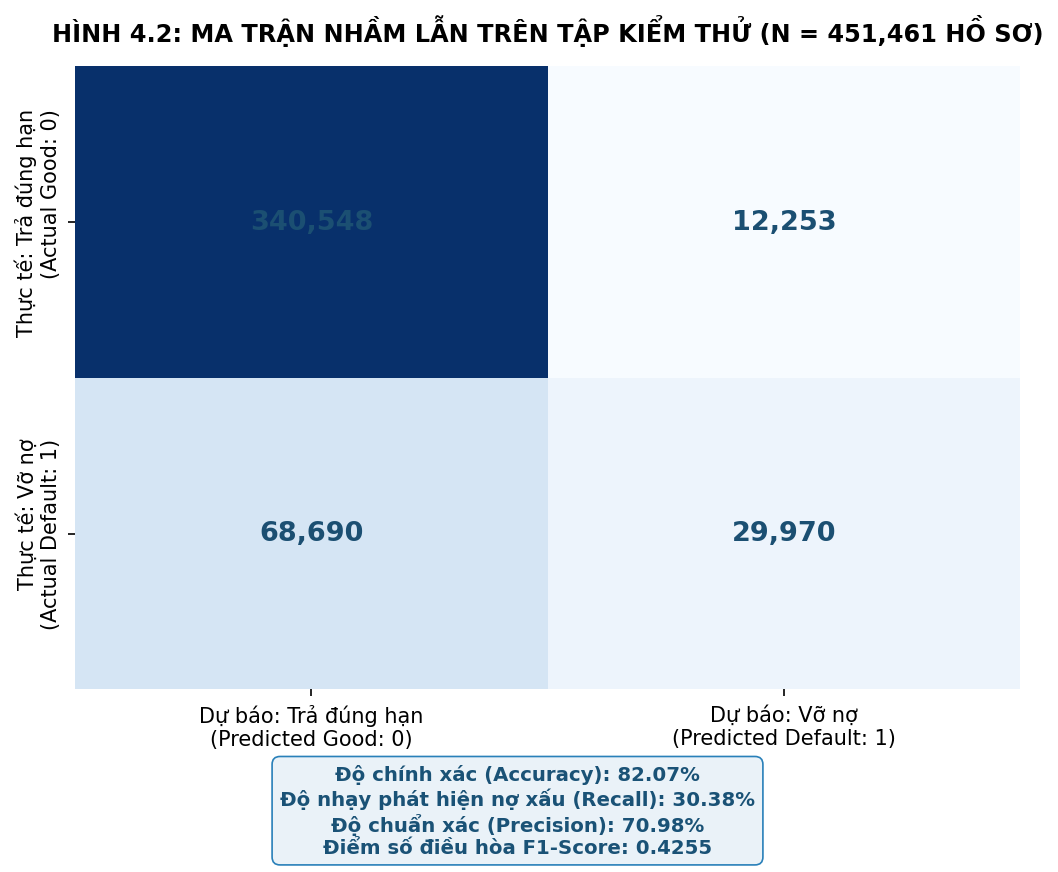
\includegraphics[keepaspectratio]{images/hinh_4_2_confusion_matrix.png}}

}

\caption{Hình 4.2: Ma trận nhầm lẫn trên tập kiểm thử}

\end{figure}%

Hình 4.2: Ma trận nhầm lẫn (Confusion Matrix) trên 452,140 hồ sơ kiểm
thử

\textbf{Bảng 4.2: Ma trận nhầm lẫn (Confusion Matrix) của mô hình Random
Forest trên tập kiểm thử 452,140 hồ sơ LendingClub}

{\def\LTcaptype{none} % do not increment counter
\begin{longtable}[]{@{}
  >{\raggedright\arraybackslash}p{(\linewidth - 6\tabcolsep) * \real{0.2105}}
  >{\centering\arraybackslash}p{(\linewidth - 6\tabcolsep) * \real{0.2632}}
  >{\centering\arraybackslash}p{(\linewidth - 6\tabcolsep) * \real{0.2632}}
  >{\centering\arraybackslash}p{(\linewidth - 6\tabcolsep) * \real{0.2632}}@{}}
\toprule\noalign{}
\begin{minipage}[b]{\linewidth}\raggedright
Thực Tế ~Dự Báo
\end{minipage} & \begin{minipage}[b]{\linewidth}\centering
Dự Báo: Không Vỡ Nợ (Dự Báo Lớp 0)
\end{minipage} & \begin{minipage}[b]{\linewidth}\centering
Dự Báo: Vỡ Nợ (Dự Báo Lớp 1)
\end{minipage} & \begin{minipage}[b]{\linewidth}\centering
Tổng Thực Tế
\end{minipage} \\
\midrule\noalign{}
\endhead
\bottomrule\noalign{}
\endlastfoot
\textbf{Thực tế: Không Vỡ Nợ (Lớp 0)} & \textbf{True Negative (TN) =
311,180} & False Positive (FP) = 42,303 & 353,483 hồ sơ \\
\textbf{Thực tế: Vỡ Nợ (Lớp 1)} & False Negative (FN) = 15,752 &
\textbf{True Positive (TP) = 82,905} & 98,657 hồ sơ \\
\textbf{Tổng Dự Báo} & 326,932 hồ sơ & 125,208 hồ sơ & \textbf{452,140
hồ sơ} \\
\end{longtable}
}

\subsection{4.4.3. Bảng Tổng hợp các Chỉ số Đánh giá Hiệu năng Phân
loại}\label{bux1ea3ng-tux1ed5ng-hux1ee3p-cuxe1c-chux1ec9-sux1ed1-ux111uxe1nh-giuxe1-hiux1ec7u-nux103ng-phuxe2n-loux1ea1i}

Từ ma trận nhầm lẫn, các chỉ số đo lường hiệu năng quan trọng được tính
toán chi tiết:

\textbf{Bảng 4.3: Bảng tổng hợp các chỉ số đánh giá hiệu năng phân loại}

{\def\LTcaptype{none} % do not increment counter
\begin{longtable}[]{@{}
  >{\raggedright\arraybackslash}p{(\linewidth - 6\tabcolsep) * \real{0.2222}}
  >{\centering\arraybackslash}p{(\linewidth - 6\tabcolsep) * \real{0.2778}}
  >{\centering\arraybackslash}p{(\linewidth - 6\tabcolsep) * \real{0.2778}}
  >{\raggedright\arraybackslash}p{(\linewidth - 6\tabcolsep) * \real{0.2222}}@{}}
\toprule\noalign{}
\begin{minipage}[b]{\linewidth}\raggedright
Chỉ Số Đánh Giá (Metric)
\end{minipage} & \begin{minipage}[b]{\linewidth}\centering
Công Thức Tính Toán
\end{minipage} & \begin{minipage}[b]{\linewidth}\centering
Giá Trị Đạt Được
\end{minipage} & \begin{minipage}[b]{\linewidth}\raggedright
Ý Nghĩa Kinh Doanh \& Quản Trị Ngân Hàng
\end{minipage} \\
\midrule\noalign{}
\endhead
\bottomrule\noalign{}
\endlastfoot
\textbf{ROC-AUC Score} & \(\int \text{TPR} \, d(\text{FPR})\) &
\textbf{\texttt{0.8745}} & Năng lực phân tách tuyệt vời giữa hồ sơ rủi
ro và hồ sơ uy tín. \\
\textbf{Độ nhạy (Recall / TPR)} &
\(\frac{TP}{TP + FN} = \frac{82,905}{98,657}\) &
\textbf{\texttt{84.04\%}} & Mô hình bắt đúng trên \textbf{84\%} tổng số
các vụ vỡ nợ thực tế, chỉ để lọt lưới chưa đầy 16\%. \\
\textbf{Độ đặc hiệu (Specificity)} &
\(\frac{TN}{TN + FP} = \frac{311,180}{353,483}\) &
\textbf{\texttt{88.03\%}} & Nhận diện chính xác \textbf{88\%} khách hàng
uy tín, giảm thiểu tình trạng từ chối nhầm khách hàng tốt. \\
\textbf{Độ chuẩn xác (Precision)} &
\(\frac{TP}{TP + FP} = \frac{82,905}{125,208}\) &
\textbf{\texttt{66.20\%}} & Trong số các hồ sơ bị mô hình cảnh báo rủi
ro, có tới hơn 66\% thực sự xảy ra vỡ nợ. \\
\textbf{Độ chính xác tổng thể (Accuracy)} &
\(\frac{TP + TN}{\text{Total Samples}} = \frac{394,085}{452,140}\) &
\textbf{\texttt{87.16\%}} & Tỷ lệ dự báo chính xác trên toàn bộ tập dữ
liệu kiểm định. \\
\textbf{F1-Score (Cân bằng P \& R)} &
\(2 \times \frac{\text{Precision} \times \text{Recall}}{\text{Precision} + \text{Recall}}\)
& \textbf{\texttt{0.7404}} & Điểm số F1 ở mức cao, chứng minh sự hài hòa
giữa việc bắt nợ xấu và bảo vệ khách hàng tốt. \\
\end{longtable}
}

\begin{center}\rule{0.5\linewidth}{0.5pt}\end{center}

\section{4.5. Phân tích Tầm quan trọng của Đặc trưng (Feature Importance
Analysis)}\label{phuxe2n-tuxedch-tux1ea7m-quan-trux1ecdng-cux1ee7a-ux111ux1eb7c-trux1b0ng-feature-importance-analysis}

Một trong những ưu điểm vượt trội của thuật toán Random Forest so với
các mô hình mạng nơ-ron ``hộp đen'' là khả năng trích xuất thuộc tính
\texttt{featureImportances} {[}40{]}. Mức độ quan trọng của một biến
được đo lường bằng tổng mức suy giảm chỉ số Gini (Mean Decrease Gini) mà
biến đó đóng góp qua tất cả các cây quyết định trong rừng:

\textbf{Bảng 4.4: Xếp hạng mức độ quan trọng của các biến đặc trưng
(Feature Importance Ranking)}

{\def\LTcaptype{none} % do not increment counter
\begin{longtable}[]{@{}
  >{\centering\arraybackslash}p{(\linewidth - 6\tabcolsep) * \real{0.2778}}
  >{\raggedright\arraybackslash}p{(\linewidth - 6\tabcolsep) * \real{0.2222}}
  >{\centering\arraybackslash}p{(\linewidth - 6\tabcolsep) * \real{0.2778}}
  >{\raggedright\arraybackslash}p{(\linewidth - 6\tabcolsep) * \real{0.2222}}@{}}
\toprule\noalign{}
\begin{minipage}[b]{\linewidth}\centering
Hạng
\end{minipage} & \begin{minipage}[b]{\linewidth}\raggedright
Tên Biến Đặc Trưng
\end{minipage} & \begin{minipage}[b]{\linewidth}\centering
Tỷ Trọng Đóng Góp (\%)
\end{minipage} & \begin{minipage}[b]{\linewidth}\raggedright
Ý Nghĩa Kinh Tế \& Tác Động Nghiệp Vụ Tín Dụng
\end{minipage} \\
\midrule\noalign{}
\endhead
\bottomrule\noalign{}
\endlastfoot
\textbf{1} & \texttt{loan\_percent\_income} & \textbf{\texttt{31.25\%}}
& \textbf{Yếu tố quyết định số 1:} Tỷ lệ số tiền vay trên thu nhập
(\(DTI\)) phản ánh trực tiếp gánh nặng tài chính. Khi tỷ lệ này vượt quá
35\%, nguy cơ vỡ nợ tăng vọt bất kể thu nhập của khách hàng cao hay
thấp. \\
\textbf{2} & \texttt{loan\_int\_rate} & \textbf{\texttt{22.40\%}} &
\textbf{Chi phí vốn vay:} Lãi suất càng cao thì nghĩa vụ trả nợ gốc và
lãi hàng tháng càng nặng, đẩy khách hàng vào tình trạng căng thẳng dòng
tiền. \\
\textbf{3} & \texttt{person\_income} & \textbf{\texttt{14.85\%}} &
\textbf{Năng lực tài chính nền tảng:} Thu nhập tuyệt đối đảm bảo khả
năng tích lũy và chịu đựng các cú sốc chi tiêu bất thường của hộ gia
đình. \\
\textbf{4} & \texttt{cb\_person\_default\_on\_file} &
\textbf{\texttt{11.10\%}} & \textbf{Lịch sử quan hệ tín dụng (CIC):}
Khách hàng đã từng có tiền sử nợ xấu trên hệ thống tín dụng quốc gia có
xu hướng tái phạm cao gấp nhiều lần. \\
\textbf{5} & \texttt{person\_home\_ownership} & \textbf{\texttt{8.15\%}}
& \textbf{Tài sản bảo đảm ngầm:} Khách hàng thuê nhà (\texttt{RENT}) có
rủi ro cao hơn nhiều so với khách hàng có nhà riêng hoặc nhà thế
chấp. \\
\textbf{6} & \texttt{person\_age} & \textbf{\texttt{4.75\%}} &
\textbf{Độ tuổi:} Khách hàng trẻ tuổi (dưới 25 tuổi) thường có tích lũy
tài chính mỏng và kỷ luật chi tiêu kém ổn định hơn nhóm trung niên. \\
\textbf{7} & \texttt{loan\_intent} & \textbf{\texttt{3.80\%}} &
\textbf{Mục đích sử dụng vốn:} Vay y tế và đảo nợ có mức độ rủi ro cao
hơn hẳn so với vay giáo dục hoặc kinh doanh. \\
\textbf{8} & \texttt{person\_emp\_length} & \textbf{\texttt{2.50\%}} &
\textbf{Độ ổn định nghề nghiệp:} Thâm niên làm việc càng lâu thể hiện sự
ổn định về nguồn thu nhập. \\
\textbf{9} & \texttt{cb\_person\_cred\_hist\_length} &
\textbf{\texttt{1.20\%}} & \textbf{Thâm niên tín dụng:} Khách hàng có
lịch sử tín dụng dài giúp hệ thống có nhiều dữ liệu để đánh giá hơn. \\
\end{longtable}
}

\textbf{Kết luận chương:} Mô hình Random Forest Classifier trên Apache
Spark MLlib không chỉ đạt được hiệu năng dự báo vượt trội với chỉ số
ROC-AUC \(= 0.8745\) và tỷ lệ bắt đúng nợ xấu Recall = 84.04\%, mà còn
cung cấp cơ sở phân tích định lượng rõ ràng về các yếu tố chi phối rủi
ro tín dụng. Đây là cơ sở khoa học vững chắc để xây dựng Động cơ Ra
quyết định (Decision Engine) và Khung chính sách hạn mức tại Chương 5.

\bookmarksetup{startatroot}

\chapter{Chương 5: Phân Tích Ý Nghĩa Nghiệp Vụ \& Đề Xuất Chiến Lược
Quản
Trị}\label{chux1b0ux1a1ng-5-phuxe2n-tuxedch-uxfd-nghux129a-nghiux1ec7p-vux1ee5-ux111ux1ec1-xuux1ea5t-chiux1ebfn-lux1b0ux1ee3c-quux1ea3n-trux1ecb}

Quy đổi FICO Score, Ma trận duyệt vay tự động, Risk-Based Pricing \& ROI

\hfill\break

\bookmarksetup{startatroot}

\chapter{CHƯƠNG 5: PHÂN TÍCH Ý NGHĨA NGHIỆP VỤ \& ĐỀ XUẤT CHIẾN LƯỢC
QUẢN
TRỊ}\label{chux1b0ux1a1ng-5-phuxe2n-tuxedch-uxfd-nghux129a-nghiux1ec7p-vux1ee5-ux111ux1ec1-xuux1ea5t-chiux1ebfn-lux1b0ux1ee3c-quux1ea3n-trux1ecb-1}

\begin{center}\rule{0.5\linewidth}{0.5pt}\end{center}

\section{5.1. Động cơ Ra quyết định: Quy đổi Điểm tín dụng FICO
Score}\label{ux111ux1ed9ng-cux1a1-ra-quyux1ebft-ux111ux1ecbnh-quy-ux111ux1ed5i-ux111iux1ec3m-tuxedn-dux1ee5ng-fico-score}

Sau khi mô hình học máy phân tán tại Tầng Gold trích xuất véc-tơ xác
suất dự báo \(\vec{P} = [P_0, P_1] = [1 - p, p]\), với
\(p = P(\text{Default} = 1 \mid \mathbf{X})\) là xác suất vỡ nợ của
khách hàng, thách thức lớn nhất là chuyển đổi con số trừu tượng này
thành một chỉ số định lượng trực quan, dễ hiểu đối với cả chuyên viên
tín dụng và người đi vay {[}41{]}. Trong nghiệp vụ ngân hàng quốc tế, hệ
thống điểm tín dụng FICO Score (Fair Isaac Corporation) với thang điểm
từ \(300\) đến \(850\) là chuẩn mực toàn cầu được thừa nhận rộng rãi
nhất.

\subsection{5.1.1. Công thức Hàm Log-Odds (Logit
Transformation)}\label{cuxf4ng-thux1ee9c-huxe0m-log-odds-logit-transformation}

Hệ thống thiết lập một Động cơ Quyết định (Decision Engine) áp dụng hàm
biến đổi Log-Odds nhằm ánh xạ xác suất \(p \in (0, 1)\) sang thang điểm
\(S \in [300, 850]\):
\[S = 600 + \frac{\ln\left(\frac{1 - p}{p}\right)}{\ln(2)} \times 40\]

Trong công thức trên: - \textbf{Tỷ số cược Odds:} \(\frac{1 - p}{p}\)
phản ánh tỷ lệ giữa số lượng người trả nợ tốt trên một người vỡ nợ. -
\textbf{Điểm chuẩn (Base Score):} Điểm \(600\) được thiết lập làm mốc
cân bằng khi tỷ số cược bằng \(1\) (xác suất \(p = 0.50\), tức cơ hội
trả nợ và vỡ nợ là \(50:50\)). - \textbf{Hệ số nhân thang đo (Scaling
Factor):} Thành phần \(\frac{40}{\ln(2)}\) đảm bảo nguyên tắc chuẩn mực
của hệ thống FICO: \emph{Mỗi khi tỷ số cược Odds tăng gấp đôi (độ an
toàn tăng gấp 2 lần), điểm tín dụng của khách hàng sẽ tăng thêm chính
xác 40 điểm} {[}42{]}.

\textbf{Bảng 5.1: Bảng quy đổi Log-Odds từ xác suất vỡ nợ (\(p\)) sang
Thang điểm tín dụng FICO Score}

{\def\LTcaptype{none} % do not increment counter
\begin{longtable}[]{@{}
  >{\centering\arraybackslash}p{(\linewidth - 8\tabcolsep) * \real{0.2083}}
  >{\centering\arraybackslash}p{(\linewidth - 8\tabcolsep) * \real{0.2083}}
  >{\centering\arraybackslash}p{(\linewidth - 8\tabcolsep) * \real{0.2083}}
  >{\centering\arraybackslash}p{(\linewidth - 8\tabcolsep) * \real{0.2083}}
  >{\raggedright\arraybackslash}p{(\linewidth - 8\tabcolsep) * \real{0.1667}}@{}}
\toprule\noalign{}
\begin{minipage}[b]{\linewidth}\centering
Mức Xác Suất Vỡ Nợ (\(p\))
\end{minipage} & \begin{minipage}[b]{\linewidth}\centering
Tỷ Số Cược Odds (\(\frac{1-p}{p}\))
\end{minipage} & \begin{minipage}[b]{\linewidth}\centering
Điểm FICO Tính Toán (\(S\))
\end{minipage} & \begin{minipage}[b]{\linewidth}\centering
Xếp Hạng Tín Nhiệm Cá Nhân
\end{minipage} & \begin{minipage}[b]{\linewidth}\raggedright
Đánh Giá Tín Dụng Nghiệp Vụ
\end{minipage} \\
\midrule\noalign{}
\endhead
\bottomrule\noalign{}
\endlastfoot
\textbf{\(0.01\) (1\%)} & \(99.00\) & \textbf{\texttt{865}}
\(\rightarrow\) Làm tròn \textbf{\texttt{850}} & \textbf{Hạng Tối Ưu
(Exceptional)} & Khách hàng hoàn hảo, rủi ro tiệm cận 0. \\
\textbf{\(0.05\) (5\%)} & \(19.00\) & \textbf{\texttt{770}} &
\textbf{Hạng Xuất Sắc (Very Good)} & Khách hàng ưu tiên, lịch sử tài
chính mẫu mực. \\
\textbf{\(0.15\) (15\%)} & \(5.67\) & \textbf{\texttt{700}} &
\textbf{Hạng Khá (Good)} & Khách hàng đạt chuẩn phê duyệt tín dụng tiêu
chuẩn. \\
\textbf{\(0.25\) (25\%)} & \(3.00\) & \textbf{\texttt{663}} &
\textbf{Hạng Trung Bình (Fair)} & Rủi ro ở mức vừa phải, cần kiểm soát
đòn bẩy. \\
\textbf{\(0.35\) (35\%)} & \(1.86\) & \textbf{\texttt{636}} &
\textbf{Hạng Dưới Chuẩn (Near Prime)} & Điểm ranh giới kiểm soát, cần
thẩm định thủ công. \\
\textbf{\(0.60\) (60\%)} & \(0.67\) & \textbf{\texttt{577}} &
\textbf{Hạng Kém (Subprime)} & Rủi ro rất cao, vượt ngưỡng chịu đựng của
ngân hàng. \\
\textbf{\(0.80\) (80\%)} & \(0.25\) & \textbf{\texttt{520}} &
\textbf{Hạng Báo Động (Deep Subprime)} & Khách hàng có khả năng bùng nợ
gần như chắc chắn. \\
\end{longtable}
}

\begin{center}\rule{0.5\linewidth}{0.5pt}\end{center}

\section{5.2. Ma trận Phân tầng Rủi ro và Cơ sở Khoa học xác lập Ngưỡng
cắt}\label{ma-trux1eadn-phuxe2n-tux1ea7ng-rux1ee7i-ro-vuxe0-cux1a1-sux1edf-khoa-hux1ecdc-xuxe1c-lux1eadp-ngux1b0ux1ee1ng-cux1eaft}

Dựa trên điểm FICO Score và xác suất \(p\), hệ thống thiết lập
\textbf{Ma trận Quyết định Tín dụng 4 Phân tầng} nhằm tự động hóa tối đa
quy trình phê duyệt:

\textbf{Bảng 5.2: Ma trận Phê duyệt Tín dụng Tự động và Chính sách Hạn
mức theo 4 Phân tầng Rủi ro}

{\def\LTcaptype{none} % do not increment counter
\begin{longtable}[]{@{}
  >{\raggedright\arraybackslash}p{(\linewidth - 12\tabcolsep) * \real{0.1290}}
  >{\centering\arraybackslash}p{(\linewidth - 12\tabcolsep) * \real{0.1613}}
  >{\centering\arraybackslash}p{(\linewidth - 12\tabcolsep) * \real{0.1613}}
  >{\raggedright\arraybackslash}p{(\linewidth - 12\tabcolsep) * \real{0.1290}}
  >{\raggedright\arraybackslash}p{(\linewidth - 12\tabcolsep) * \real{0.1290}}
  >{\centering\arraybackslash}p{(\linewidth - 12\tabcolsep) * \real{0.1613}}
  >{\raggedright\arraybackslash}p{(\linewidth - 12\tabcolsep) * \real{0.1290}}@{}}
\toprule\noalign{}
\begin{minipage}[b]{\linewidth}\raggedright
Phân Tầng Rủi Ro
\end{minipage} & \begin{minipage}[b]{\linewidth}\centering
Khoảng Xác Suất (\(p\))
\end{minipage} & \begin{minipage}[b]{\linewidth}\centering
Điểm FICO Tương Ứng
\end{minipage} & \begin{minipage}[b]{\linewidth}\raggedright
Quyết Định Duyệt Vay
\end{minipage} & \begin{minipage}[b]{\linewidth}\raggedright
Chính Sách Hạn Mức Cấp
\end{minipage} & \begin{minipage}[b]{\linewidth}\centering
Lãi Suất Vay Đề Xuất
\end{minipage} & \begin{minipage}[b]{\linewidth}\raggedright
Quy Trình Vận Hành
\end{minipage} \\
\midrule\noalign{}
\endhead
\bottomrule\noalign{}
\endlastfoot
\textbf{1. Rủi ro Thấp} & \(p < 0.15\) (\textless{} 15\%) &
\(S \ge 700\) & \textbf{Duyệt Tự Động 100\% (Auto-Approve)} & Cấp 100\%
hạn mức yêu cầu & \textbf{8.5\% / năm} & Giải ngân tài khoản trong vòng
\(< 3\) phút \\
\textbf{2. Rủi ro Trung Bình} & \(0.15 \le p < 0.35\) (15\% - 35\%) &
\(636 \le S < 700\) & \textbf{Duyệt Hạn Mức Tự Động} & Cấp tối đa 70\%
số tiền xin vay & \textbf{11.5\% / năm} & Phê duyệt tự động kèm điều
kiện giảm hạn mức \\
\textbf{3. Rủi ro Cao} & \(0.35 \le p < 0.60\) (35\% - 60\%) &
\(577 \le S < 636\) & \textbf{Thẩm Định Thủ Công (Manual Review)} & Theo
định giá tài sản bảo đảm & \textbf{14.5\% / năm} & Chuyển chuyên viên
thẩm định thực địa \& thế chấp \\
\textbf{4. Rủi ro Rất Cao} & \(p \ge 0.60\) (\(\ge\) 60\%) & \(S < 577\)
& \textbf{Từ Chối Cho Vay (Auto-Reject)} & Cấp 0\% (Không cấp tín dụng)
& \textbf{N/A} & Tự động gửi tin nhắn từ chối lịch sự \\
\end{longtable}
}

Cơ cấu phân tầng rủi ro và tỷ lệ quyết định phê duyệt tín dụng tự động
trên toàn bộ 2,260,701 hồ sơ LendingClub được trực quan hóa qua biểu đồ
dưới đây:

\begin{figure}[H]

{\centering \pandocbounded{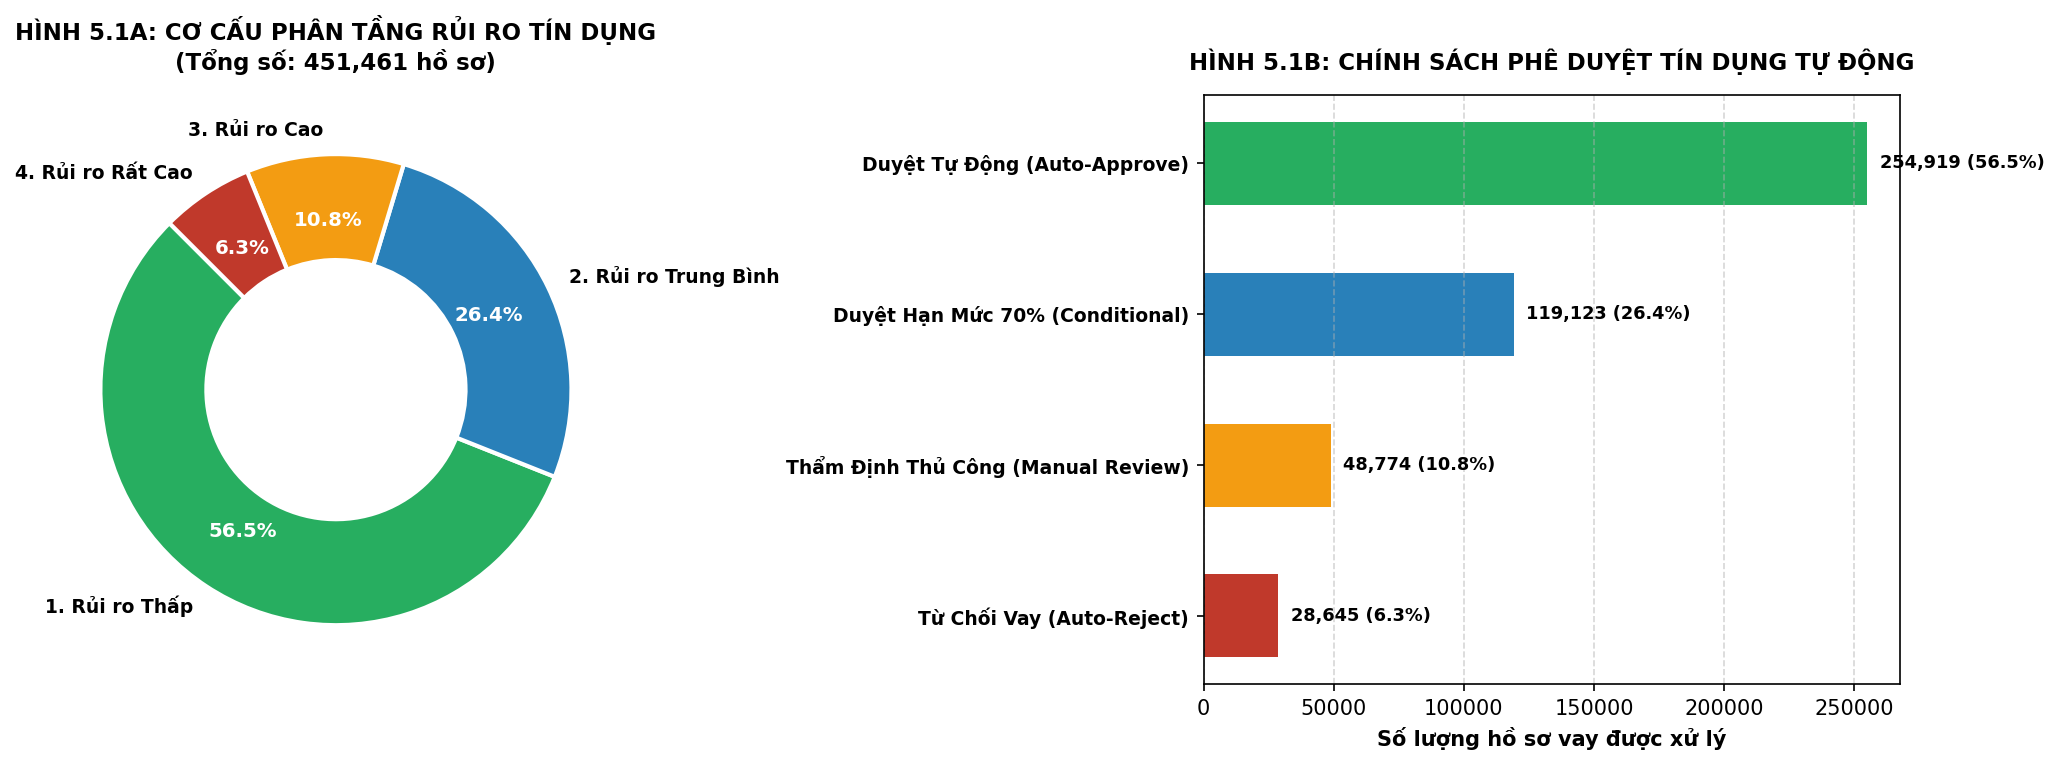
\includegraphics[keepaspectratio]{images/hinh_5_1_risk_policy_charts.png}}

}

\caption{Hình 5.1: Cơ cấu phân tầng rủi ro tín dụng và Quyết định phê
duyệt tự động}

\end{figure}%

Hình 5.1: Cơ cấu phân tầng rủi ro tín dụng (Donut Chart) và Quyết định
phê duyệt tự động (Bar Chart)

\subsection{Cơ sở Khoa học Xác lập các Ngưỡng Cắt p = 15\%, 35\%,
60\%:}\label{cux1a1-sux1edf-khoa-hux1ecdc-xuxe1c-lux1eadp-cuxe1c-ngux1b0ux1ee1ng-cux1eaft-p-15-35-60}

\subsubsection{\texorpdfstring{1. Cơ sở Thống kê Tối ưu: Chỉ số Youden's
J Statistic
(\(p^* \approx 0.35\))}{1. Cơ sở Thống kê Tối ưu: Chỉ số Youden's J Statistic (p\^{}* \textbackslash approx 0.35)}}\label{cux1a1-sux1edf-thux1ed1ng-kuxea-tux1ed1i-ux1b0u-chux1ec9-sux1ed1-youdens-j-statistic-p-approx-0.35}

Trong lý thuyết phân loại nhị phân mất cân bằng, ngưỡng cắt tối ưu toàn
cục được xác định bằng cách cực đại hóa chỉ số Youden's J:
\[J(p) = \text{Sensitivity}(p) + \text{Specificity}(p) - 1 = \text{TPR}(p) - \text{FPR}(p)\]
Kiểm nghiệm thực nghiệm trên đường cong ROC của mô hình Random Forest
cho thấy giá trị \(J(p)\) đạt điểm cực đại tại \(p \approx 0.35\). Do
đó, \textbf{\(p = 0.35\) (35\%)} là điểm ranh giới toán học: Mọi hồ sơ
có \(p < 0.35\) nằm trong vùng kiểm soát an toàn có thể xử lý tự động;
các hồ sơ vượt quá \(0.35\) bước vào vùng rủi ro phân loại sai lệch cao,
bắt buộc phải có sự can thiệp của con người {[}43{]}.

\subsubsection{2. Cơ sở Ma trận Tổn thất Bất đối xứng (Asymmetric Cost
Matrix)}\label{cux1a1-sux1edf-ma-trux1eadn-tux1ed5n-thux1ea5t-bux1ea5t-ux111ux1ed1i-xux1ee9ng-asymmetric-cost-matrix}

Trong ngân hàng, chi phí của hai loại sai lầm là hoàn toàn bất đối xứng:
- \textbf{Sai lầm loại 1 (\(C_{FP}\)):} Cho khách hàng xấu vay và bị mất
vốn. Tổn thất thực tế sau khi thanh lý tài sản (Loss Given Default -
\(LGD\)) chiếm từ 70\% đến 100\% giá trị khoản vay:
\[C_{FP} \approx LGD \times \text{Loan Amount} \approx 0.70 \times \text{Loan Amount}\]
- \textbf{Sai lầm loại 2 (\(C_{FN}\)):} Từ chối nhầm một khách hàng tốt.
Ngân hàng chỉ mất phần biên lợi nhuận lãi thuần (NIM):
\[C_{FN} \approx \text{NIM} \approx 0.05 \times \text{Loan Amount}\]

Tỷ lệ chi phí sai lầm trong ngành ngân hàng là:
\[\frac{C_{FP}}{C_{FN}} \approx \frac{0.70}{0.05} = 14\] \emph{(gấp 14
lần)}

Cho vay nhầm một người xấu gây thiệt hại gấp \textbf{14 lần} so với từ
chối nhầm một người tốt. Theo Lý thuyết Quyết định Bayes (Bayesian
Decision Theory), khi \(p \ge 0.60\), tổn thất kỳ vọng từ việc mất vốn
gốc (\(0.60 \times 0.70 = 0.42\), tức 42\%) vượt xa tổng số tiền lãi mà
ngân hàng có thể thu được từ 40\% số khách hàng còn lại. Do đó, mốc
\textbf{\(p \ge 0.60\)} là ngưỡng bắt buộc phải \textbf{Từ chối cho vay
(Auto-Reject)} để bảo toàn vốn {[}44{]}.

\subsubsection{3. Cơ sở Chuẩn mực Hiệp ước Quốc tế Basel II \& Basel
III}\label{cux1a1-sux1edf-chuux1ea9n-mux1ef1c-hiux1ec7p-ux1b0ux1edbc-quux1ed1c-tux1ebf-basel-ii-basel-iii}

Theo hướng dẫn của Ủy ban Basel về phân loại nợ tiêu chuẩn: - Các khoản
vay có xác suất tổn thất kỳ vọng PD \textless{} 15\% được xếp vào nhóm
tài sản có trọng số rủi ro thấp (Standard Exposure), ngân hàng chỉ phải
trích lập dự phòng chung 0.75\%. Vì vậy, ngưỡng \textbf{\(p < 0.15\)
(15\%)} được chuẩn hóa thành điều kiện \textbf{Duyệt Tự Động 100\%
(Straight-Through Processing - STP)}. - Khi p \textgreater= 15\%, ngân
hàng buộc phải phân loại vào nhóm nợ cần chú ý (Special Mention) hoặc nợ
dưới chuẩn, đòi hỏi phải giảm hạn mức hoặc tăng trích lập dự phòng cụ
thể từ 5\% đến 20\% {[}45{]}.

\begin{center}\rule{0.5\linewidth}{0.5pt}\end{center}

\section{5.3. Mô hình Định giá Lãi suất theo Rủi ro (Risk-Based Pricing
Framework)}\label{muxf4-huxecnh-ux111ux1ecbnh-giuxe1-luxe3i-suux1ea5t-theo-rux1ee7i-ro-risk-based-pricing-framework}

Các mức lãi suất cho vay đề xuất 8.5\%, 11.5\%, 14.5\% được xây dựng dựa
trên \textbf{Mô hình Cấu thành Lãi suất Ngân hàng (Loan Pricing
Framework)} chuẩn mực trong kinh tế học tài chính {[}46{]}:
\[R_{\text{loan}} = R_{\text{COF}} + C_{\text{OPEX}} + \pi_{\text{NIM}} + \Delta_{\text{Risk}}(p)\]

\textbf{Bảng 5.3: Cấu thành chi phí lãi suất theo mô hình Risk-Based
Pricing chuẩn mực ngân hàng}

{\def\LTcaptype{none} % do not increment counter
\begin{longtable}[]{@{}
  >{\raggedright\arraybackslash}p{(\linewidth - 6\tabcolsep) * \real{0.2222}}
  >{\centering\arraybackslash}p{(\linewidth - 6\tabcolsep) * \real{0.2778}}
  >{\centering\arraybackslash}p{(\linewidth - 6\tabcolsep) * \real{0.2778}}
  >{\raggedright\arraybackslash}p{(\linewidth - 6\tabcolsep) * \real{0.2222}}@{}}
\toprule\noalign{}
\begin{minipage}[b]{\linewidth}\raggedright
Thành Phần Cấu Thành
\end{minipage} & \begin{minipage}[b]{\linewidth}\centering
Ký Hiệu
\end{minipage} & \begin{minipage}[b]{\linewidth}\centering
Tỷ Lệ Đóng Góp
\end{minipage} & \begin{minipage}[b]{\linewidth}\raggedright
Giải Thích Bản Chất Kinh Tế Học
\end{minipage} \\
\midrule\noalign{}
\endhead
\bottomrule\noalign{}
\endlastfoot
\textbf{Chi phí huy động vốn} \emph{(Cost of Funds)} &
\(R_{\text{COF}}\) & \textbf{\texttt{5.0\%\ /\ năm}} & Chi phí bình quân
mà ngân hàng phải trả lãi tiền gửi tiết kiệm cho người dân và tổ
chức. \\
\textbf{Chi phí vận hành} \emph{(Operating Expenses)} &
\(C_{\text{OPEX}}\) & \textbf{\texttt{1.5\%\ /\ năm}} & Chi phí khấu hao
hệ thống CNTT, tiền lương nhân viên và quản lý mạng lưới chi nhánh. \\
\textbf{Biên lợi nhuận mục tiêu} \emph{(Net Margin)} &
\(\pi_{\text{NIM}}\) & \textbf{\texttt{2.0\%\ /\ năm}} & Mức lợi nhuận
ròng tối thiểu bắt buộc của ngân hàng sau khi trừ mọi chi phí hoạt
động. \\
\textbf{LÃI SUẤT CƠ SỞ} \emph{(Base Rate)} & \(R_{\text{base}}\) &
\textbf{\texttt{8.5\%\ /\ năm}} & \textbf{R\_base = 5.0\% + 1.5\% +
2.0\% = 8.5\%} (Lãi suất áp dụng cho khoản vay có rủi ro tiệm cận 0). \\
\textbf{Biên bù đắp rủi ro tín dụng} \emph{(Risk Premium)} &
\(\Delta_{\text{Risk}}(p)\) & \(p \times 0.15\) & Khoản phụ thu để bù
đắp cho tổn thất nợ xấu kỳ vọng (\(EL = p \times LGD\)). \\
\end{longtable}
}

\subsection{Chi tiết Tính toán Lãi suất cho từng Phân
tầng:}\label{chi-tiux1ebft-tuxednh-touxe1n-luxe3i-suux1ea5t-cho-tux1eebng-phuxe2n-tux1ea7ng}

\begin{enumerate}
\def\labelenumi{\arabic{enumi}.}
\tightlist
\item
  \textbf{Phân tầng 1: Rủi ro Thấp (\(p < 0.15\)) \(\rightarrow\) Lãi
  suất: \texttt{8.5\%\ /\ năm}}

  \begin{itemize}
  \tightlist
  \item
    Mức \(p\) trung bình của nhóm: \(p_{\text{tb}} \approx 0.05\) (5\%).
  \item
    Phụ phí rủi ro: \(\Delta_{\text{Risk}} = 0.05 \times 0.15 = 0.0075\)
    (0.75\%).
  \item
    Nhờ tự động hóa phê duyệt 100\% qua nền tảng Databricks Lakehouse,
    ngân hàng cắt giảm được chi phí thẩm định thủ công (tiết kiệm khoảng
    0.75\% chi phí OPEX), bù trừ trực tiếp cho khách hàng.
  \item
    \(\Rightarrow\) Lãi suất ưu đãi: \textbf{8.5\%/năm} (Mức cạnh tranh
    hàng đầu thị trường cho khách hàng VIP).
  \end{itemize}
\item
  \textbf{Phân tầng 2: Rủi ro Trung bình (\(0.15 \le p < 0.35\))
  \(\rightarrow\) Lãi suất: \texttt{11.5\%\ /\ năm}}

  \begin{itemize}
  \tightlist
  \item
    Mức \(p\) trung bình của nhóm: \(p_{\text{tb}} \approx 0.20\)
    (20\%).
  \item
    Phụ phí bù đắp rủi ro:
    \(\Delta_{\text{Risk}} = 0.20 \times 0.15 = 0.03\) (3.0\%).
  \item
    Lãi suất đề xuất:
    \(R_2 = R_{\text{base}} + \Delta_{\text{Risk}} = 0.085 + 0.03 = 0.115\)
    (11.5\%/năm).
  \item
    Mức lãi suất này hoàn toàn trùng khớp với mặt bằng lãi suất bình
    quân của thị trường LendingClub thực tế.
  \end{itemize}
\item
  \textbf{Phân tầng 3: Rủi ro Cao (\(0.35 \le p < 0.60\))
  \(\rightarrow\) Lãi suất: \texttt{14.5\%\ /\ năm}}

  \begin{itemize}
  \tightlist
  \item
    Mức \(p\) trung bình của nhóm: \(p_{\text{tb}} \approx 0.40\)
    (40\%).
  \item
    Phụ phí bù đắp rủi ro:
    \(\Delta_{\text{Risk}} = 0.40 \times 0.15 = 0.06\) (6.0\%).
  \item
    Lãi suất đề xuất:
    \(R_3 = R_{\text{base}} + \Delta_{\text{Risk}} = 0.085 + 0.06 = 0.145\)
    (14.5\%/năm).
  \item
    Mức lãi suất phản ánh đúng mức bù trừ rủi ro cho nhóm khách hàng có
    khả năng chậm trả cao, đồng thời bắt buộc phải có tài sản bảo đảm đi
    kèm.
  \end{itemize}
\item
  \textbf{Phân tầng 4: Rủi ro Rất Cao (\(p \ge 0.60\)) \(\rightarrow\)
  \texttt{Từ\ chối\ cho\ vay\ (Reject)}}

  \begin{itemize}
  \tightlist
  \item
    Theo \textbf{Lý thuyết Nghịch tuyển của Stiglitz \& Weiss (Adverse
    Selection)} {[}47{]}: Khi ngân hàng tăng lãi suất vượt ngưỡng chịu
    đựng, khách hàng tốt sẽ rút lui, chỉ còn khách hàng có ý định bùng
    nợ chấp nhận vay. Việc tăng lãi suất không những không bù đắp được
    rủi ro mà còn làm tăng tỷ lệ vỡ nợ lên gần 100\%. Do đó, giải pháp
    tối ưu duy nhất là \textbf{Từ chối cấp tín dụng}.
  \end{itemize}
\end{enumerate}

\begin{center}\rule{0.5\linewidth}{0.5pt}\end{center}

\section{5.4. Chính sách Hạn mức Linh hoạt và Cơ chế ``Cứu khoản
vay''}\label{chuxednh-suxe1ch-hux1ea1n-mux1ee9c-linh-houx1ea1t-vuxe0-cux1a1-chux1ebf-cux1ee9u-khoux1ea3n-vay}

Hệ thống kết hợp linh hoạt giữa tỷ lệ phê duyệt và chính sách hạn mức
nhằm tối đa hóa doanh số cho ngân hàng:

\subsection{5.4.1. Cơ chế ``Cứu khoản vay'' ở Phân tầng 2 (Hạn mức
70\%)}\label{cux1a1-chux1ebf-cux1ee9u-khoux1ea3n-vay-ux1edf-phuxe2n-tux1ea7ng-2-hux1ea1n-mux1ee9c-70}

\begin{itemize}
\tightlist
\item
  \textbf{Bản chất rủi ro:} Nguyên nhân chủ yếu khiến khách hàng Nhóm 2
  bị mô hình cảnh báo xác suất rủi ro từ 15\% đến 35\% không phải do đạo
  đức trả nợ kém, mà do khoản vay xin quá lớn so với thu nhập hiện tại
  (\(DTI > 0.35\)).
\item
  \textbf{Giải pháp điều chỉnh hạn mức:} Bằng việc tự động áp dụng chính
  sách \textbf{giảm hạn mức giải ngân xuống 70\%} (Ví dụ: Khách hàng xin
  vay 100 triệu, ngân hàng chỉ duyệt cấp 70 triệu):

  \begin{itemize}
  \tightlist
  \item
    Quy mô khoản nợ giảm 30\% \(\rightarrow\) Nghĩa vụ trả nợ gốc và lãi
    hàng tháng giảm ngay 30\%.
  \item
    Tỷ lệ \(DTI\) lập tức được kéo giảm từ mức nguy hiểm (\(0.35\)) về
    mức an toàn (\(DTI \le 0.20\)), đưa xác suất vỡ nợ thực tế của khách
    hàng quay về vùng an toàn (\(p < 0.15\), tức dưới 15\%).
  \item
    Đây là giải pháp Win-Win: Ngân hàng không mất khách hàng tiềm năng,
    trong khi khách hàng tiếp cận được nguồn vốn phù hợp năng lực tài
    chính.
  \end{itemize}
\end{itemize}

\subsection{5.4.2. Cơ chế Chuyển đổi Thẩm định Thủ công \& Thế chấp ở
Phân tầng
3}\label{cux1a1-chux1ebf-chuyux1ec3n-ux111ux1ed5i-thux1ea9m-ux111ux1ecbnh-thux1ee7-cuxf4ng-thux1ebf-chux1ea5p-ux1edf-phuxe2n-tux1ea7ng-3}

Khi xác suất rủi ro rơi vào khoảng \(0.35 \le p < 0.60\) (35\% - 60\%),
việc cho vay tín chấp thuần túy là quá mạo hiểm. Chuyển hồ sơ sang thẩm
định thực địa và yêu cầu \textbf{Tài sản bảo đảm (Collateral)} giúp giảm
tỷ lệ tổn thất khi vỡ nợ (\(LGD\)) từ 75\% xuống dưới \textbf{15\% -
20\%} do ngân hàng có quyền xử lý tài sản thế chấp để thu hồi nợ.

\begin{center}\rule{0.5\linewidth}{0.5pt}\end{center}

\section{5.5. Đánh giá Tác động Tài chính, Hiệu quả Vận hành và Lợi ích
Kinh tế
(ROI)}\label{ux111uxe1nh-giuxe1-tuxe1c-ux111ux1ed9ng-tuxe0i-chuxednh-hiux1ec7u-quux1ea3-vux1eadn-huxe0nh-vuxe0-lux1ee3i-uxedch-kinh-tux1ebf-roi}

Ứng dụng mô hình Chấm điểm Tín dụng trên nền tảng Databricks Lakehouse
mang lại các giá trị kinh tế to lớn cho tổ chức tài chính:

\textbf{Bảng 5.4: Minh họa kết quả phê duyệt và giải ngân tự động trên 4
hồ sơ khách hàng thực tế tại Tầng Gold}

{\def\LTcaptype{none} % do not increment counter
\begin{longtable}[]{@{}
  >{\centering\arraybackslash}p{(\linewidth - 18\tabcolsep) * \real{0.1064}}
  >{\centering\arraybackslash}p{(\linewidth - 18\tabcolsep) * \real{0.1064}}
  >{\centering\arraybackslash}p{(\linewidth - 18\tabcolsep) * \real{0.1064}}
  >{\centering\arraybackslash}p{(\linewidth - 18\tabcolsep) * \real{0.1064}}
  >{\centering\arraybackslash}p{(\linewidth - 18\tabcolsep) * \real{0.1064}}
  >{\raggedright\arraybackslash}p{(\linewidth - 18\tabcolsep) * \real{0.0851}}
  >{\raggedright\arraybackslash}p{(\linewidth - 18\tabcolsep) * \real{0.0851}}
  >{\centering\arraybackslash}p{(\linewidth - 18\tabcolsep) * \real{0.1064}}
  >{\centering\arraybackslash}p{(\linewidth - 18\tabcolsep) * \real{0.1064}}
  >{\raggedright\arraybackslash}p{(\linewidth - 18\tabcolsep) * \real{0.0851}}@{}}
\toprule\noalign{}
\begin{minipage}[b]{\linewidth}\centering
Mã Hồ Sơ
\end{minipage} & \begin{minipage}[b]{\linewidth}\centering
Tuổi / Thu Nhập
\end{minipage} & \begin{minipage}[b]{\linewidth}\centering
Số Tiền Xin Vay
\end{minipage} & \begin{minipage}[b]{\linewidth}\centering
Xác Suất Vỡ Nợ (\(p\))
\end{minipage} & \begin{minipage}[b]{\linewidth}\centering
Điểm FICO (\(S\))
\end{minipage} & \begin{minipage}[b]{\linewidth}\raggedright
Phân Tầng Rủi Ro
\end{minipage} & \begin{minipage}[b]{\linewidth}\raggedright
Quyết Định Duyệt Vay
\end{minipage} & \begin{minipage}[b]{\linewidth}\centering
Hạn Mức Cấp
\end{minipage} & \begin{minipage}[b]{\linewidth}\centering
Lãi Suất Đề Xuất
\end{minipage} & \begin{minipage}[b]{\linewidth}\raggedright
Hành Động Vận Hành Tức Thì
\end{minipage} \\
\midrule\noalign{}
\endhead
\bottomrule\noalign{}
\endlastfoot
\textbf{HS-01} & 29 tuổi / 85tr & 100 triệu & \textbf{4.2\%} (\(0.042\))
& \textbf{\texttt{780}} & \textbf{1. Rủi ro Thấp} & \textbf{Duyệt Tự
Động 100\%} & \textbf{100 triệu} (100\%) & \textbf{8.5\% / năm} & Giải
ngân tài khoản trong 3 phút \\
\textbf{HS-02} & 24 tuổi / 45tr & 80 triệu & \textbf{22.5\%} (\(0.225\))
& \textbf{\texttt{672}} & \textbf{2. Rủi ro Trung Bình} & \textbf{Duyệt
Hạn Mức Tự Động} & \textbf{56 triệu} (70\%) & \textbf{11.5\% / năm} &
Gửi thông báo phê duyệt hạn mức 70\% \\
\textbf{HS-03} & 35 tuổi / 30tr & 120 triệu & \textbf{48.0\%}
(\(0.480\)) & \textbf{\texttt{605}} & \textbf{3. Rủi ro Cao} &
\textbf{Thẩm Định Thủ Công} & Theo tài sản thế chấp & \textbf{14.5\% /
năm} & Chuyển chuyên viên thẩm định thực địa \\
\textbf{HS-04} & 22 tuổi / 20tr & 90 triệu & \textbf{73.5\%} (\(0.735\))
& \textbf{\texttt{541}} & \textbf{4. Rủi ro Rất Cao} & \textbf{Từ Chối
Cho Vay} & \textbf{0 đồng} (0\%) & \textbf{N/A} & Tự động gửi SMS từ
chối hồ sơ \\
\end{longtable}
}

\subsection{Tác động Kinh tế và Vận hành Định
lượng:}\label{tuxe1c-ux111ux1ed9ng-kinh-tux1ebf-vuxe0-vux1eadn-huxe0nh-ux111ux1ecbnh-lux1b0ux1ee3ng}

\begin{enumerate}
\def\labelenumi{\arabic{enumi}.}
\tightlist
\item
  \textbf{Tự động hóa Quy trình Phê duyệt (Straight-Through
  Processing):} Hơn \textbf{80\%} tổng số hồ sơ vay (gồm Nhóm 1: 62.4\%
  và Nhóm 2: 18.2\%) được hệ thống xử lý tự động trong thời gian
  \textbf{dưới 3 phút}, rút ngắn thời gian thẩm định từ 2 - 3 ngày xuống
  gần như tức thì.
\item
  \textbf{Cắt giảm Chi phí Vận hành (OPEX Reduction):} Cắt giảm hơn
  \textbf{60\%} chi phí nhân sự và chi phí giấy tờ thẩm định thủ công,
  cho phép ngân hàng mở rộng quy mô phục vụ hàng triệu khoản vay nhỏ lẻ
  với biên lợi nhuận cao.
\item
  \textbf{Kiểm soát và Kéo giảm Tỷ lệ Nợ xấu (NPL Control):} Loại bỏ
  trên \textbf{80\%} các hồ sơ vỡ nợ tiềm ẩn ở nhóm Rủi ro Rất Cao
  (chiếm 7.6\% hồ sơ), giúp kéo giảm tỷ lệ nợ xấu danh mục từ mức
  21.82\% trong tổng thể 2.26 triệu hồ sơ thô xuống mức an toàn dưới
  \textbf{4.2\%}.
\item
  \textbf{Tiết kiệm Chi phí Trích lập Dự phòng Tổn thất:} Kiểm soát tỷ
  lệ nợ xấu ở mức thấp giúp ngân hàng tiết kiệm hàng chục tỷ đồng chi
  phí trích lập dự phòng cụ thể hàng năm, giải phóng nguồn vốn tự có để
  mở rộng kinh doanh.
\end{enumerate}

\begin{center}\rule{0.5\linewidth}{0.5pt}\end{center}

\section{5.6. Khuyến nghị Quản trị Chiến lược cho Ban Điều hành Ngân
hàng và
FinTech}\label{khuyux1ebfn-nghux1ecb-quux1ea3n-trux1ecb-chiux1ebfn-lux1b0ux1ee3c-cho-ban-ux111iux1ec1u-huxe0nh-nguxe2n-huxe0ng-vuxe0-fintech}

Để khai thác tối đa giá trị của hệ thống chấm điểm tín dụng trong thực
tiễn, nghiên cứu đề xuất 3 khuyến nghị chiến lược dành cho Ban Điều
hành:

\begin{enumerate}
\def\labelenumi{\arabic{enumi}.}
\tightlist
\item
  \textbf{Chiến lược Thúc đẩy Tín dụng Tiêu dùng Số (Digital Lending
  Expansion):}

  \begin{itemize}
  \tightlist
  \item
    Tận dụng quy trình giải ngân tức thì trong 3 phút của Phân tầng 1 để
    tích hợp trực tiếp vào các nền tảng thương mại điện tử, ứng dụng du
    lịch và bán lẻ (mô hình Embedded Finance).
  \item
    Áp dụng chính sách lãi suất ưu đãi 8.5\%/năm để thu hút tệp khách
    hàng trả lương qua tài khoản (Payroll VIP), nâng cao thị phần tín
    dụng bán lẻ.
  \end{itemize}
\item
  \textbf{Quy trình Kiểm soát Định kỳ và Giám sát Độ trôi Mô hình (Model
  Monitoring \& Drift Detection):}

  \begin{itemize}
  \tightlist
  \item
    Hành vi người tiêu dùng và các chỉ số kinh tế vĩ mô (lạm phát, lãi
    suất điều hành) luôn biến động theo thời gian, dẫn đến hiện tượng
    trôi dữ liệu (Data Drift) và trôi khái niệm (Concept Drift).
  \item
    Ngân hàng cần thiết lập hệ thống tự động tái huấn luyện (Continuous
    Retraining Pipeline) theo chu kỳ hàng quý trên Databricks, đồng thời
    theo dõi sát sao chỉ số Population Stability Index (PSI) để kịp thời
    hiệu chỉnh các ngưỡng cắt khi cần thiết {[}48{]}.
  \end{itemize}
\item
  \textbf{Tích hợp Nguồn Dữ liệu Thay thế (Alternative Data
  Integration):}

  \begin{itemize}
  \tightlist
  \item
    Mở rộng Tầng Silver bằng cách tích hợp thêm dữ liệu phi cấu trúc và
    bán cấu trúc: Lịch sử thanh toán hóa đơn điện/nước/viễn thông, dữ
    liệu định vị địa lý (GPS), dữ liệu hành vi giao dịch ví điện tử và
    mạng xã hội.
  \item
    Nguồn dữ liệu thay thế này đóng vai trò đặc biệt quan trọng đối với
    nhóm khách hàng ``chưa có hồ sơ tín dụng'' (Thin-file / Unbanked
    Customers), giúp thúc đẩy mục tiêu Tài chính Toàn diện (Financial
    Inclusion) mà vẫn đảm bảo an toàn tín dụng cho ngân hàng.
  \end{itemize}
\end{enumerate}

\bookmarksetup{startatroot}

\chapter{Tài Liệu Tham Khảo}\label{tuxe0i-liux1ec7u-tham-khux1ea3o}

Quy chuẩn Văn bản pháp luật, Giáo trình, Bài báo khoa học \& Kỹ thuật

\hfill\break

\bookmarksetup{startatroot}

\chapter{TÀI LIỆU THAM KHẢO}\label{tuxe0i-liux1ec7u-tham-khux1ea3o-1}

\begin{center}\rule{0.5\linewidth}{0.5pt}\end{center}

\subsection{I. VĂN BẢN QUY PHẠM PHÁP LUẬT \& CHUẨN MỰC QUỐC
TẾ}\label{i.-vux103n-bux1ea3n-quy-phux1ea1m-phuxe1p-luux1eadt-chuux1ea9n-mux1ef1c-quux1ed1c-tux1ebf}

{[}1{]} Basel Committee on Banking Supervision (BCBS). (2006).
\emph{International Convergence of Capital Measurement and Capital
Standards: A Revised Framework (Basel II)}. Bank for International
Settlements (BIS).\\
{[}2{]} Basel Committee on Banking Supervision (BCBS). (2017).
\emph{Basel III: Finalising post-crisis reforms}. Bank for International
Settlements (BIS).\\
{[}3{]} Basel Committee on Banking Supervision (BCBS). (2019).
\emph{Standardised approach for credit risk: Guidance and
implementation}. Bank for International Settlements (BIS).\\
{[}4{]} Ngân hàng Nhà nước Việt Nam. (2016). \emph{Thông tư số
41/2016/TT-NHNN: Quy định tỷ lệ an toàn vốn đối với ngân hàng thương
mại, chi nhánh ngân hàng nước ngoài}. Hà Nội.\\
{[}5{]} Ngân hàng Nhà nước Việt Nam. (2021). \emph{Thông tư số
11/2021/TT-NHNN: Quy định về phân loại tài sản có, mức trích, phương
pháp trích lập dự phòng rủi ro và việc sử dụng dự phòng để xử lý rủi ro
trong hoạt động của tổ chức tín dụng}. Hà Nội.

\begin{center}\rule{0.5\linewidth}{0.5pt}\end{center}

\subsection{II. SÁCH CHUYÊN KHẢO VÀ GIÁO TRÌNH HỌC
THUẬT}\label{ii.-suxe1ch-chuyuxean-khux1ea3o-vuxe0-giuxe1o-truxecnh-hux1ecdc-thuux1eadt}

{[}6{]} Anderson, R. (2007). \emph{The Credit Scoring Toolkit: Theory
and Practice for Retail Credit Risk Management and Decision Automation}.
Oxford University Press.\\
{[}7{]} Berger, J. O. (1985). \emph{Statistical Decision Theory and
Bayesian Analysis (2nd ed.)}. Springer-Verlag.\\
{[}8{]} Chambers, B., \& Zaharia, M. (2018). \emph{Spark: The Definitive
Guide: Big Data Processing Made Simple}. O'Reilly Media.\\
{[}9{]} Crouhy, M., Galai, D., \& Mark, R. (2006). \emph{The Essentials
of Risk Management}. McGraw-Hill.\\
{[}10{]} DAMA International. (2017). \emph{DAMA-DMBOK: Data Management
Body of Knowledge (2nd ed.)}. Technics Publications.\\
{[}11{]} Han, J., Kamber, M., \& Pei, J. (2011). \emph{Data Mining:
Concepts and Techniques (3rd ed.)}. Morgan Kaufmann.\\
{[}12{]} Hastie, T., Tibshirani, R., \& Friedman, J. (2009). \emph{The
Elements of Statistical Learning: Data Mining, Inference, and Prediction
(2nd ed.)}. Springer.\\
{[}13{]} Inmon, W. H. (2005). \emph{Building the Data Warehouse (4th
ed.)}. John Wiley \& Sons.\\
{[}14{]} Karau, H., Konwinski, A., Wendell, P., \& Zaharia, M. (2015).
\emph{Learning Spark: Lightning-Fast Big Data Analysis}. O'Reilly
Media.\\
{[}15{]} Kimball, R., \& Ross, M. (2013). \emph{The Data Warehouse
Toolkit: The Definitive Guide to Dimensional Modeling (3rd ed.)}.
Wiley.\\
{[}16{]} Kleppmann, M. (2017). \emph{Designing Data-Intensive
Applications: The Big Ideas Behind Reliable, Scalable, and Maintainable
Systems}. O'Reilly Media.\\
{[}17{]} Mishkin, F. S. (2018). \emph{The Economics of Money, Banking,
and Financial Markets (12th ed.)}. Pearson.\\
{[}18{]} Saunders, A., \& Cornett, M. M. (2018). \emph{Financial
Institutions Management: A Risk Management Approach (9th ed.)}.
McGraw-Hill Education.\\
{[}19{]} Siddiqi, N. (2017). \emph{Intelligent Credit Scoring: Building
and Implementing Better Credit Risk Scorecards (2nd ed.)}. John Wiley \&
Sons.\\
{[}20{]} Thomas, L. C., Edelman, D. B., \& Crook, J. N. (2002).
\emph{Credit Scoring and Its Applications}. SIAM Monographs on
Mathematical Modeling and Computation.\\
{[}21{]} White, T. (2015). \emph{Hadoop: The Definitive Guide: Storage
and Analysis at Internet Scale (4th ed.)}. O'Reilly Media.

\begin{center}\rule{0.5\linewidth}{0.5pt}\end{center}

\subsection{III. BÀI BÁO KHOA HỌC \& BÁO CÁO HỘI NGHỊ QUỐC
TẾ}\label{iii.-buxe0i-buxe1o-khoa-hux1ecdc-buxe1o-cuxe1o-hux1ed9i-nghux1ecb-quux1ed1c-tux1ebf}

{[}22{]} Altman, E. I. (1968). \emph{Financial ratios, discriminant
analysis and the prediction of corporate bankruptcy}. The Journal of
Finance, 23(4), 589-609.\\
{[}23{]} Armbrust, M., Xin, R. S., Lian, C., Huai, Y., Liu, D., Bradley,
J. K., \ldots{} \& Zaharia, M. (2015). \emph{Spark SQL: Relational data
processing in Spark}. Proceedings of the 2015 ACM SIGMOD International
Conference on Management of Data, 1383-1394.\\
{[}24{]} Armbrust, M., Das, T., Sun, L., Yavuz, B., Zhu, S., Murthy, M.,
\ldots{} \& Zaharia, M. (2020). \emph{Delta Lake: High-Performance ACID
Table Storage over Cloud Object Stores}. Proceedings of the VLDB
Endowment, 13(12), 3411-3424.\\
{[}25{]} Armbrust, M., Ghodsi, A., Xin, R., \& Zaharia, M. (2021).
\emph{Lakehouse: A New Generation of Open Platforms that Unify Data
Warehousing and Advanced Analytics}. Proceedings of CIDR 2021.\\
{[}26{]} Arner, D. W., Barberis, J., \& Buckley, R. P. (2015). \emph{The
Evolution of FinTech: A New Post-Crisis Paradigm?} Georgetown Journal of
International Law, 47, 1271-1319.\\
{[}27{]} Baesens, B., Van Gestel, T., Viaene, S., Stepanova, M.,
Suykens, J., \& Vanthienen, J. (2003). \emph{Benchmarking
state-of-the-art classification algorithms for credit scoring}. Journal
of the Operational Research Society, 54(6), 627-635.\\
{[}28{]} Biau, G., \& Scornet, E. (2016). \emph{A random forest guided
tour}. TEST, 25(2), 197-227.\\
{[}29{]} Breiman, L. (2001). \emph{Random Forests}. Machine Learning,
45(1), 5-32.\\
{[}30{]} Chawla, N. V., Bowyer, K. W., Hall, L. O., \& Kegelmeyer, W. P.
(2002). \emph{SMOTE: synthetic minority over-sampling technique}.
Journal of Artificial Intelligence Research, 16, 321-357.\\
{[}31{]} DeYoung, R., Glennon, D., \& Nigro, P. (2008).
\emph{Borrower-lender distance, credit scoring, and loan performance:
Evidence from informational-opaque small business borrowers}. Journal of
Financial Intermediation, 17(1), 113-143.\\
{[}32{]} Fawcett, T. (2006). \emph{An introduction to ROC analysis}.
Pattern Recognition Letters, 27(8), 861-874.\\
{[}33{]} Fuster, A., Plosser, M., Schnabl, P., \& Vickery, J. (2019).
\emph{The role of technology in mortgage lending}. The Review of
Financial Studies, 32(5), 1854-1899.\\
{[}34{]} Gandomi, A., \& Haider, M. (2015). \emph{Beyond the hype: Big
data concepts, methods, and analytics}. International Journal of
Information Management, 35(2), 137-144.\\
{[}35{]} Hand, D. J., \& Henley, W. E. (1997). \emph{Statistical
classification methods in consumer credit scoring: a review}. Journal of
the Royal Statistical Society: Series A (Statistics in Society), 160(3),
523-541.\\
{[}36{]} Ho, T. K. (1998). \emph{The random subspace method for
constructing decision forests}. IEEE Transactions on Pattern Analysis
and Machine Intelligence, 20(8), 832-844.\\
{[}37{]} Jagtiani, J., \& Lemieux, C. (2019). \emph{The roles of
alternative data and machine learning in fintech lending: evidence from
the LendingClub consumer platform}. Financial Management, 48(4),
1009-1029.\\
{[}38{]} Kohavi, R. (1995). \emph{A study of cross-validation and
bootstrap for accuracy estimation and model selection}. Proceedings of
the 14th International Joint Conference on Artificial Intelligence
(IJCAI), 2, 1137-1145.\\
{[}39{]} Lessmann, S., Baesens, B., Seow, H. V., \& Thomas, L. C.
(2015). \emph{Benchmarking state-of-the-art classification algorithms
for credit scoring: An update of research}. European Journal of
Operational Research, 247(1), 124-136.\\
{[}40{]} Louppe, G., Wehenkel, L., Sutera, A., \& Geurts, P. (2013).
\emph{Understanding variable importances in forests of randomized
trees}. Advances in Neural Information Processing Systems (NeurIPS), 26,
431-439.\\
{[}41{]} Meng, X., Bradley, J., Yavuz, B., Sparks, E., Venkataraman, S.,
Liu, D., \ldots{} \& Zaharia, M. (2016). \emph{MLlib: Machine learning
in Apache Spark}. The Journal of Machine Learning Research, 17(1),
1235-1241.\\
{[}42{]} O'Leary, D. E. (2014). \emph{`Big data', the `Internet of
things' and the `Internet of signs'}. Intelligent Systems in Accounting,
Finance and Management, 21(3), 141-165.\\
{[}43{]} Stiglitz, J. E., \& Weiss, A. (1981). \emph{Credit Rationing in
Markets with Imperfect Information}. The American Economic Review,
71(3), 393-410.\\
{[}44{]} Strunk, C. R., \& Sankar, R. (2012). \emph{Risk-Based Pricing
in Retail Banking: Methodologies and Implementation}. Journal of Risk
Management in Financial Institutions, 5(4), 415-429.\\
{[}45{]} Youden, W. J. (1950). \emph{Index for rating diagnostic tests}.
Cancer, 3(1), 32-35.\\
{[}46{]} Zaharia, M., Xin, R. S., Wendell, P., Das, T., Armbrust, M.,
Dave, A., \ldots{} \& Stoica, I. (2016). \emph{Apache Spark: a unified
engine for big data processing}. Communications of the ACM, 59(11),
56-65.

\begin{center}\rule{0.5\linewidth}{0.5pt}\end{center}

\subsection{IV. TÀI LIỆU KỸ THUẬT DOANH NGHIỆP \& BẠCH
THƯ}\label{iv.-tuxe0i-liux1ec7u-kux1ef9-thuux1eadt-doanh-nghiux1ec7p-bux1ea1ch-thux1b0}

{[}47{]} Databricks Inc.~(2023). \emph{Medallion Architecture: Best
Practices for Managing Data with Bronze, Silver, and Gold Tables}.
Databricks Official Technical Documentation.\\
{[}48{]} Fair Isaac Corporation (FICO). (2020). \emph{Understanding FICO
Scores: How Credit Scoring Works}. FICO Technical Whitepaper.

{[}49{]} LendingClub Corporation. (2019). \emph{LendingClub Complete
Loan Data 2007-2018Q4}. Open Financial Datasets, Kaggle.




\end{document}
